\section{Group -- Airflow Network}\label{group-airflow-network}

\subsection{Overview}\label{overview}

The Airflow Network model provides the ability to simulate multizone airflows driven by wind and also by forced air distribution systems. The model can also simulate the heat and moisture gains or losses from the air distribution system itself (e.g., ductwork). When modeling air distribution systems, the current version of the Airflow Network model is allowed to simulate multiple forced air systems (i.e., \hyperref[airloophvac]{AirLoopHVAC} object). Each forced air system allows a constant volume supply air fan (\hyperref[fanconstantvolume]{Fan:ConstantVolume} or \hyperref[fanonoff]{Fan:OnOff}), a VAV supply air fan (\hyperref[fanvariablevolume]{Fan:VariableVolume}), or a fan system model \hyperref[fansystemmodel]({Fan:SystemMode}). The capabilities of the model are to:

\begin{itemize}
\item
  Simulate zone pressures due to envelope leakage and forced air distribution during HVAC system fan operation
\item
  Simulate node pressures in a forced air distribution system during HVAC system fan operation
\item
  Calculate multizone airflows due to forced air, wind, and surface leakage, including adjacent zones and outdoors, during HVAC system fan operation
\item
  Simulate distribution system airflows, including supply and return air leaks, during HVAC system fan operation
\item
  Simulate air distribution system node temperatures and humidity ratios during HVAC system fan operation
\item
  Calculate duct conduction losses during HVAC system fan operation
\item
  Calculate vapor diffusion losses of ducts during HVAC system fan operation
\item
  Calculate sensible and latent loads on the surrounding zones due to supply and return air leaks in the air distribution system during HVAC system fan operation
\item
  Simulate zone pressures due to envelope leakage driven by wind when the HVAC system fan is off or if no air distribution system is specified
\item
  Calculate multizone airflows due to wind and surface leakage, including adjacent zones and outdoors when the HVAC system fan is off or if no air distribution system is specified
\item
  Allow zone exhaust fans to be included as part of the airflow network
\item
  For airflow networks with a forced air distribution system, calculate zone sensible and latent loads for two different supply air fan operation modes as required: cycling fan, cycling compressor (CyclingFanAndCompressor) and continuous fan, cycling compressor (ContinuousFanWithCyclingCompressor)
\item
  When multiple forced air systems (AirloopHVAC) are present in the idf, all systems must be used in the Airflow Network model.
\end{itemize}

\subsection{Summary of Objects}\label{summary-of-objects}

Before describing the Airflow Network input objects in detail, we list all of the objects and then give a short description of what the objects do.

The Airflow Network input objects are:

\textbf{\hyperref[airflownetworksimulationcontrol]{AirflowNetwork:\hyperref[simulationcontrol]{SimulationControl}}}

\textbf{\hyperref[airflownetworkmultizonezone]{AirflowNetwork:MultiZone:Zone}}

\textbf{\hyperref[airflownetworkmultizonesurface]{AirflowNetwork:MultiZone:Surface}}

\textbf{\hyperref[airflownetworkmultizonecomponentsimpleopening]{AirflowNetwork:MultiZone:Component:SimpleOpening}}

\textbf{\hyperref[airflownetworkmultizonecomponentdetailedopening]{AirflowNetwork:MultiZone:Component:DetailedOpening}}

\textbf{\hyperref[airflownetworkmultizonecomponenthorizontalopening]{AirflowNetwork:MultiZone:Component:HorizontalOpening}}

\textbf{\hyperref[airflownetworkmultizonesurfacecrack]{AirflowNetwork:MultiZone:Surface:Crack}}

\textbf{\hyperref[airflownetworkmultizonereferencecrackconditions]{AirflowNetwork:MultiZone:ReferenceCrackConditions}}

\textbf{\hyperref[airflownetworkmultizonesurfaceeffectiveleakagearea]{AirflowNetwork:MultiZone:Surface:EffectiveLeakageArea}}

\textbf{\hyperref[airflownetworkmultizonecomponentzoneexhaustfan]{AirflowNetwork:MultiZone:Component:ZoneExhaustFan}}

\textbf{\hyperref[airflownetworkmultizoneexternalnode]{AirflowNetwork:MultiZone:ExternalNode}}

\textbf{\hyperref[airflownetworkmultizonewindpressurecoefficientarray]{AirflowNetwork:MultiZone:WindPressureCoefficientArray}}

\textbf{\hyperref[airflownetworkmultizonewindpressurecoefficientvalues]{AirflowNetwork:MultiZone:WindPressureCoefficientValues}}

\textbf{\hyperref[airflownetworkintrazonenode]{AirflowNetwork:IntraZone:Node}}

\textbf{\hyperref[airflownetworkintrazonelinkage]{AirflowNetwork:IntraZone:Linkage}}

\textbf{\hyperref[airflownetworkdistributionnode]{AirflowNetwork:Distribution:Node}}

\textbf{\hyperref[airflownetworkdistributioncomponentleak]{AirflowNetwork:Distribution:Component:Leak}}

\textbf{\hyperref[airflownetworkdistributioncomponentleakageratio]{AirflowNetwork:Distribution:Component:LeakageRatio}}

\textbf{\hyperref[airflownetworkdistributioncomponentduct]{AirflowNetwork:Distribution:Component:Duct}}

\textbf{\hyperref[airflownetworkdistributioncomponentconstantpressuredrop]{AirflowNetwork:Distribution:Component:ConstantPressureDrop}}

\textbf{\hyperref[airflownetworkdistributioncomponentfan]{AirflowNetwork:Distribution:Component:Fan}}

\textbf{\hyperref[airflownetworkdistributioncomponentcoil]{AirflowNetwork:Distribution:Component:Coil}}

\textbf{\hyperref[airflownetworkdistributioncomponentheatexchanger]{AirflowNetwork:Distribution:Component:HeatExchanger}}

\textbf{\hyperref[airflownetworkdistributioncomponentterminalunit]{AirflowNetwork:Distribution:Component:TerminalUnit}}

\textbf{\hyperref[airflowNetworkdistributioncomponentoutdoorairflow]{AirflowNetwork:Distribution:Component:OutdoorAirFlow}}

\textbf{\hyperref[airflowNetworkdistributioncomponentreliefairflow]{AirflowNetwork:Distribution:Component:ReliefAirFlow}}

\textbf{\hyperref[airflownetworkdistributionlinkage]{AirflowNetwork:Distribution:Linkage}}

\textbf{~}

\begin{itemize}
\item
  \textbf{\hyperref[airflownetworksimulationcontrol]{AirflowNetwork:\hyperref[simulationcontrol]{SimulationControl}}} defines basic run parameters for the air flow calculations and specifies whether wind pressure coefficients are input by the user or, for rectangular buildings, calculated by the program.
\item
  The \textbf{\hyperref[airflownetworkmultizonezone]{AirflowNetwork:MultiZone:Zone}} object specifies the ventilation control that applies to all of the openable exterior and interior windows and doors in the corresponding thermal zone. Surface-level ventilation control can be used to override the zone-level ventilation control if required (see AirflowNetwork: MultiZone:Surface object below).
\item
  \textbf{\hyperref[airflownetworkmultizonesurface]{AirflowNetwork:MultiZone:Surface}} object indicates whether a heat transfer surface (wall, window, etc.) has a crack or opening and references an object in the list below that gives the air flow characteristics of that crack, opening, or zone exhaust fan. The \hyperref[airflownetworkmultizonesurface]{AirflowNetwork:MultiZone:Surface} object can also be used to specify individual ventilation control for openable exterior and interior windows and doors.
\begin{itemize}
\item \textbf{\hyperref[airflownetworkmultizonesurfacecrack]{AirflowNetwork:MultiZone:Surface:Crack}
\item \hyperref[airflownetworkmultizonesurfaceeffectiveleakagearea]{AirflowNetwork:Multi-Zone:Surface:EffectiveLeakageArea}
\item \hyperref[airflownetworkmultizonecomponentsimpleopening]{AirflowNetwork:MultiZone:Component:SimpleOpening}
\item \hyperref[airflownetworkmultizonecomponentdetailedopening]{AirflowNetwork:Multi-Zone:Component:DetailedOpening}
\item \hyperref[airflownetworkmultizonecomponenthorizontalopening]{AirflowNetwork:MultiZone:Component:HorizontalOpening}
\item \hyperref[airflownetworkmultizonecomponentzoneexhaustfan]{AirflowNetwork:Multi-Zone:Component:ZoneExhaustFan}}
\end{itemize}
\item
  \textbf{\hyperref[airflownetworkmultizonereferencecrackconditions]{AirflowNetwork:MultiZone:ReferenceCrackConditions}} is used to normalize crack information that is based on measurements of crack air flow.
\item
  \textbf{\hyperref[airflownetworkdistributionnode]{AirflowNetwork:Distribution:Node}} represents air distribution system nodes for the AirflowNetwork model. A set of an \hyperref[airloophvac]{AirLoopHVAC} and \hyperref[zonehvacequipmentlist]{ZoneHVAC:EquipmentList} nodes is a subset of the \hyperref[airflownetworkdistributionnode]{AirflowNetwork:Distribution:Node}s.
\item
  \textbf{AirflowNetwork:Distribution:Component} objects consist of \textbf{Leak, LeakageRatio, Duct, ConstantPressureDrop, Fan, Coil, TerminalUnit, OutdoorAirFlow} and \textbf{ReliefAirFlow.} The components provide a relationship between pressure and airflow. The \textbf{Leak} and \textbf{Leakage} components can be used to simulate supply and/or return leaks in an air distribution system\textbf{.} The \textbf{Duct} and \textbf{ConstantPressureDrop components} can be used to deliver forced air into conditioned spaces. The components \textbf{Fan, Coil, and TerminalUnit} reference normal EnergyPlus objects. \textbf{OutdoorAirFlow, and ReliefAirFlow} specify the outdoor air flow rate set by the \hyperref[controlleroutdoorair]{Controller:OutdoorAir} object in the model. The Airflow Network model gets information from these objects to perform an airflow network simulation.
\item
  \textbf{\hyperref[airflownetworkdistributionlinkage]{AirflowNetwork:Distribution:Linkage}} object represents a connection between two node objects and an AirflowNetwork component. The node objects can be an \hyperref[airflownetworkdistributionnode]{AirflowNetwork:Distribution:Node}, \hyperref[airflownetworkmultizoneexternalnode]{AirflowNetwork:MultiZone:ExternalNode} or \hyperref[airflownetworkmultizonezone]{AirflowNetwork:MultiZone:Zone}.
\end{itemize}

If you input wind pressure coefficients, \textbf{\hyperref[airflownetworkmultizonesurface]{AirflowNetwork:MultiZone:Surface}} also has an associated \textbf{\hyperref[airflownetworkmultizoneexternalnode]{AirflowNetwork:MultiZone:ExternalNode}}, that, via the \textbf{\hyperref[airflownetworkmultizonewindpressurecoefficientarray]{AirflowNetwork:MultiZone:Wind-PressureCoefficientArray}} and \textbf{\hyperref[airflownetworkmultizonewindpressurecoefficientvalues]{AirflowNetwork:MultiZone:WindPressureCoefficientValues}} objects, gives the wind pressure distribution vs. wind direction for that node and, implicitly, for the cracks and openings in the exterior surfaces associated with that node.

Figure~\ref{fig:relationships-among-airflownetwork-objects} shows the relationships among AirflowNetwork:MultiZone objects and between AirflowNetwork:MultiZone objects and regular EnergyPlus objects. In this figure an arrow from object A to object B means A references B, i.e., one of the inputs in A is the name of object B. For example, one input for AirflowNetwork: MultiZone:Surface is the name of a heat transfer surface, and another is the name of a crack or opening object. The arrow between \hyperref[airflownetworkmultizonesurface]{AirflowNetwork:MultiZone:Surface} and \hyperref[airflownetworkmultizoneexternalnode]{AirflowNetwork:MultiZone:ExternalNode} is shown dashed to indicate that this reference is not used when wind pressure coefficients are calculated by the program rather than being input by the user.

Figure~\ref{fig:relationships-among-airflownetwork-objects} also shows the relationships among AirflowNetwork:Distribution objects and between AirflowNetwork:Distribution objects and regular EnergyPlus objects. The \hyperref[airflownetworkdistributionlinkage]{AirflowNetwork:Distribution:Linkage} objects link two nodes from \hyperref[airflownetworkdistributionnode]{AirflowNetwork:Distribution:Node} and/or \hyperref[airflownetworkmultizonezone]{AirflowNetwork:MultiZone:Zone} objects with a component defined in the object AirflowNetwork:Distribution:Component. The solid arrows show a reference from object A to object B. The dashed arrows indicate the components which can be used in a linkage object. The red arrows pointing to the Zone object indicate the components that interact with the zone air. For example, the temperature in a zone where a supply leak terminates is used to calculate duct leakage energy loss. The temperature in a zone where a duct component is located is also used to calculate duct conduction loss.

\begin{figure}[hbtp] % fig 93
\centering
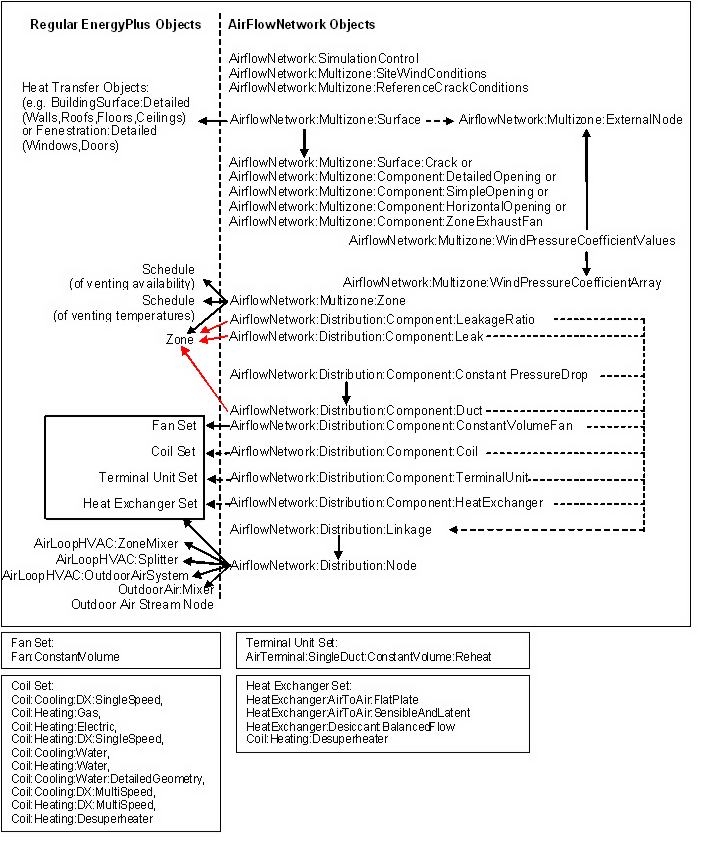
\includegraphics[width=0.9\textwidth, height=0.9\textheight, keepaspectratio=true]{media/image215.png}
\caption{Relationships among AirflowNetwork objects (right-hand side) and between AirflowNetwork objects and regular EnergyPlus objects. An arrow from object A to object B means that A references B. \protect \label{fig:relationships-among-airflownetwork-objects}}
\end{figure}

Much of the information needed for the air flow calculation is automatically extracted from the building description for thermal modeling. This includes things like the volume and neutral height of the zones, and the orientation and location of the building surfaces that contain cracks or openings through which air flows. From all of this information the program creates a ``pressure-flow network'' that is solved each timestep using iterative solution methods to obtain the unknown pressures and air flows.

Figure~\ref{fig:plan-view-of-a-simple-air-flow-network} shows a plan view of a very simple air flow network that you can construct using the above AirflowNetwork objects. There are three thermal zones, Zone-1, Zone-2 and Zone-3. There are openable exterior windows---Window-1, Window-2 and Window-3---and openable interior doors---Door-12 and Door-23. Two External Nodes are indicated. ExternalNode-1 is associated with the fa\c{c}ade that contains Window-1 and Window-2. ExternalNode-2 is associated with the fa\c{c}ade containing Window-3.

One possible air flow pattern is shown in this figure. The actual air flow pattern in a particular timestep, and the size of the flows, depends on many factors, such as (1) What is the wind pressure distribution seen by the exterior windows? (2) Are the exterior windows open or closed, and if open, how far are they open? (3) Are the interior doors open or closed? (4) What are the air temperature differences between zones and between zones and the outdoor air (which affect buoyancy flows)?

\begin{figure}[hbtp] % fig 94
\centering
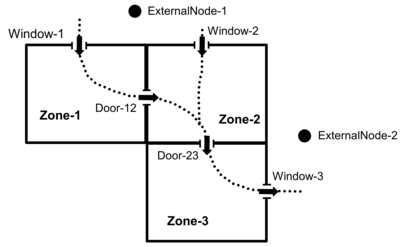
\includegraphics[width=0.9\textwidth, height=0.9\textheight, keepaspectratio=true]{media/image216.png}
\caption{Plan view of a simple air flow network showing a possible air flow pattern in which all of the windows and doors are open. \protect \label{fig:plan-view-of-a-simple-air-flow-network}}
\end{figure}

Figure~\ref{fig:plan-view-of-a-simple-air-flow-network} shows a possible air flow pattern in which all of the windows and doors are open. Associated with the external nodes are wind pressure coefficient distributions as a function of wind direction that are input using two AirflowNetwork:MultiZone:Wind Pressure Coefficient objects. The nature of the air flows through the windows and doors is specified using \hyperref[airflownetworkmultizonecomponentdetailedopening]{AirflowNetwork:MultiZone:Component:DetailedOpening} and \hyperref[airflownetworkmultizonecomponentsimpleopening]{AirflowNetwork:MultiZone:Component:SimpleOpening} objects. The Airflow Network model calculates the flows each system timestep depending on various factors, including wind direction and speed, size and vertical position of openings, outdoor air temperature, and zone air temperatures.

\subsection{Airflow Network Example Files (included in the installation)}\label{airflow-network-example-files-included-in-the-installation}

\begin{itemize}
\item
  AirflowNetwork3zVent.idf
\item
  AirflowNetwork3zVentAutoWPC.idf
\item
  AirflowNetworkOccupantVentilationControl.idf
\item
  AirflowNetwork\_Attic\_Duct.idf
\item
  AirflowNetwork\_Simple\_House.idf
\item
  AirflowNetwork\_Simple\_SmallOffice.idf
\item
  AirflowNetwork\_MultiAirLoops.idf
\item
  AirflowNetwork\_MultiZone\_House.idf
\item
  AirflowNetwork\_MultiZone\_House\_OvercoolDehumid.idf
\item
  AirflowNetwork\_MultiZone\_House\_TwoSpeed.idf
\item
  AirflowNetwork\_MultiZone\_LocalNode.idf
\item
  AirflowNetwork\_MultiZone\_SmallOffice.idf
\item
  AirflowNetwork\_MultiZone\_SmallOffice\_CoilHXAssistedDX.idf
\item
  AirflowNetwork\_MultiZone\_SmallOffice\_GenericContam.idf
\item
  AirflowNetwork\_MultiZone\_SmallOffice\_HeatRecoveryHXSL.idf
\item
  AirflowNetwork\_MultiZone\_SmallOffice\_VAV.idf
\item
  AirflowNetwork\_MultiZone\_HorizontalOpening.idf
\item
  AirflowNetwor\_PressureControl.idf
\item
  CrossVent\_1Zone\_AirflowNetwork.idf
\item
  CrossVent\_1Zone\_AirflowNetwork\_with2CrossflowJets.idf
\item
  DisplacementVent\_Nat\_AirflowNetwork.idf
\item
  DisplacementVent\_Nat\_AirflowNetwork\_AdaptiveComfort.idf
\item
  EMSAirflowNetworkOpeningControlByHumidity.idf
\item
  HybridVentilationControl.idf
\item
  RoomAirflowNetwork.idf
\end{itemize}

\subsection{What the Airflow Network Model Can and Cannot Do}\label{what-the-airflow-network-model-can-and-cannot-do}

Here is a list of some of the things that the Airflow Network calculation can and cannot model.

\subsubsection{Can Do}\label{can-do}
\begin{enumerate}
\item Air flow through cracks in exterior or interzone surfaces.
\item Air flow through cracks around windows and doors when closed.
\item Natural ventilation (i.e., air flow through open or partially open exterior windows and doors).
\item Zone level control of natural ventilation (all windows/doors in a zone that are defined with a component opening object have identical controls).
\item Individual surface control of natural ventilation for a subsurface (window, door, or glassdoor).
\item Modulation of natural ventilation to prevent large zone air temperature swings.
\item Interzone air flow (i.e., air flow through open interzone windows and doors, and through cracks in interzone surfaces).
\item Dependence of air flow on buoyancy effects and wind pressure.
\item Dependence of wind pressure on wind speed, wind direction and surface orientation.
\item Supply and return air leaks in an air distribution system.
\item Account for the effect of supply-air and/or return-air leakage on zone pressure when a forced air distribution system is present and is operating.
\item When duct leakage is modeled and the HVAC system is on, interzone airflow or infiltration/exfiltration can occur due to changes in zone pressure.
\item Bi-directional flow through large openings. See discussion below under \hyperref[airflownetworkmultizonecomponentdetailedopening]{AirflowNetwork:MultiZone:Component:DetailedOpening}, \hyperref[airflownetworkmultizonecomponenthorizontalopening]{AirflowNetwork:MultiZone:Component:HorizontalOpening}, and \hyperref[airflownetworkmultizonecomponentsimpleopening]{AirflowNetwork:MultiZone:Component:SimpleOpening}.
\item Calculate air flows and pressures in ducts or other components of a forced air distribution system.
\item Calculate zone loads when the supply air fan cycles on and off during a system timestep using the CyclingFanAndCompressor fan operation mode (\hyperref[fanonoff]{Fan:OnOff}).
\item Determine the impact of zone exhaust fans on air flows, pressures, air temperatures/humidity levels and energy consumption.
\end{enumerate}

\subsubsection{Cannot Do or Restricted}\label{cannot-do-or-restricted}
\begin{enumerate}
\item The model is restricted to using a constant volume or variable volume fan (\hyperref[fanconstantvolume]{Fan:ConstantVolume}, \hyperref[fanonoff]{Fan:OnOff}, and \hyperref[fanvariablevolume]{Fan:VariableVolume}).
\item Air circulation and/or air temperature stratification within a thermal zone. For example, you should not try to divide a high space, such as an atrium, into subzones separated by artificial horizontal surfaces that have cracks or openings with the expectation that AirflowNetwork will give you a realistic temperature in each subzone and/or a realistic air flow between subzones.
\item The model is restricted to eleven types of coils that can be in the air distribution system (\hyperref[coilcoolingdxsinglespeed]{Coil:Cooling:DX:SingleSpeed}, \hyperref[coilheatinggas-000]{Coil:Heating:Fuel}, \hyperref[coilheatingelectric]{Coil:Heating:Electric},~ \hyperref[coilheatingdxsinglespeed]{Coil:Heating:DX:SingleSpeed}, \hyperref[coilcoolingwater]{Coil:Cooling:Water}, \hyperref[coilheatingwater]{Coil:Heating:Water}, \hyperref[coilcoolingwaterdetailedgeometry]{Coil:Cooling:Water:DetailedGeometry}, \hyperref[coilcoolingdxtwostagewithhumiditycontrolmode]{Coil:Cooling:DX:TwoStageWithHumidityControlMode}, \hyperref[coilcoolingdxmultispeed]{Coil:Cooling:DX:MultiSpeed}, \hyperref[coilheatingdxmultispeed]{Coil:Heating:DX:MultiSpeed}, and \hyperref[coilheatingdesuperheater]{Coil:Heating:Desuperheater}).
\item The model is restricted to two types of air distribution equipment terminal units (\hyperref[airterminalsingleductconstantvolumereheat]{AirTerminal:SingleDuct:ConstantVolume:Reheat} and \hyperref[airterminalsingleductvavreheat]{AirTerminal:SingleDuct:VAV:Reheat}).
\item Supply and return leaks are not allowed in an \hyperref[airloophvac]{AirLoopHVAC}. They can only be modeled in the Zone Equipment portion of the air loop (i.e., return leaks may be modeled between the zone return node and the zone mixer inlet or the zone mixer outlet and the zone equipment loop outlet; and supply leaks may be modeled between the zone equipment loop inlet and the \hyperref[airloophvaczonesplitter]{AirLoopHVAC:ZoneSplitter} inlet node or the \hyperref[airloophvaczonesplitter]{AirLoopHVAC:ZoneSplitter} outlet node and the zone supply node).
\item An air distribution system must be located inside the building (i.e., the ducts must pass through zones within the building).
\item Zone exhaust fans must be defined in \hyperref[zonehvacequipmentconnections]{ZoneHVAC:EquipmentConnections} objects.
\end{enumerate}

The input specifications consist of five main sections: \textbf{\hyperref[airflownetworksimulationcontrol]{AirflowNetwork:\hyperref[simulationcontrol]{SimulationControl}} object, AirflowNetwork multizone data objects, AirflowNetwork distribution node objects, AirflowNetwork distribution component objects,} and \textbf{AirflowNetwork distribution linkage objects.} Each of these object types is described in detail below.

\subsection{AirflowNetwork:SimulationControl}\label{airflownetworksimulationcontrol}

The basic run parameters for this model are defined in this unique object which has the following input specifications:

\subsubsection{Inputs}\label{inputs-004}

\paragraph{Field: Name}\label{field-name-004}

This is a unique character string associated with this instance of the AirflowNetwork:\hyperref[simulationcontrol]{SimulationControl} object. At this time, only one AirflowNetwork:\hyperref[simulationcontrol]{SimulationControl} object can be specified in an input data file (idf).

\paragraph{Field: AirflowNetwork Control}\label{field-airflownetwork-control}

The following selections are available to control the Airflow Network simulation:

\textbf{MultiZoneWithDistribution:} MultiZone air flow calculations are performed during all simulation timesteps, including the impacts of the air distribution system when a HVAC system fan is operating. Any \textbf{ZoneInfiltration:*}, \textbf{ZoneVentilation:*}, \textbf{\hyperref[zonemixing]{ZoneMixing}} and \textbf{\hyperref[zonecrossmixing]{ZoneCrossMixing}} objects specified in the input data file are not simulated.

\textbf{MultiZoneWithoutDistribution}: MultiZone air flow calculations are performed during all simulation timesteps, but the air distribution system portion of the network is not modeled even if it is specified in the input data file. Any \textbf{ZoneInfiltration:*}, \textbf{ZoneVentilation:*}, \textbf{\hyperref[zonemixing]{ZoneMixing}} and \textbf{\hyperref[zonecrossmixing]{ZoneCrossMixing}} objects specified in the input data file are not simulated.

\textbf{MultiZoneWithDistributionOnlyDuringFanOperation:} MultiZone air flow calculations, including the impacts of the air distribution system, are only performed when the HVAC system fan is operating. Any \textbf{ZoneInfiltration:*}, \textbf{ZoneVentilation:*}, \textbf{\hyperref[zonemixing]{ZoneMixing}} and \textbf{\hyperref[zonecrossmixing]{ZoneCrossMixing}} objects specified in the input data file are used when the HVAC system fan is OFF (if none are specified, then no air flow calculations are performed when the fan is OFF).

\textbf{NoMultiZoneOrDistribution:} No multizone air flow calculations (with or without the air distribution system portion of the network) are performed during the simulation. Any \textbf{ZoneInfiltration:*}, \textbf{ZoneVentilation:*}, \textbf{\hyperref[zonemixing]{ZoneMixing}} and \textbf{\hyperref[zonecrossmixing]{ZoneCrossMixing}} objects specified in the input data file are simulated (if none are specified, then no air flow calculations are performed). Note: Having an input data file with no AirflowNetwork:\hyperref[simulationcontrol]{SimulationControl} objects gives the same impact -- no multizone air flow calculations. However, this choice is provided as a convenience to the user to easily disable the multizone air flow calculations for an input data file that already contains AirflowNetwork objects.

\textbf{Note:} A \textbf{ZoneInfiltration:*} object indicates any one of \textbf{\hyperref[zoneinfiltrationdesignflowrate]{ZoneInfiltration:DesignFlowRate}}, \textbf{\hyperref[zoneinfiltrationeffectiveleakagearea]{ZoneInfiltration:EffectiveLeakageArea}},and \textbf{\hyperref[zoneinfiltrationflowcoefficient]{ZoneInfiltration:FlowCoefficient}} objects.A object of\textbf{ZoneVentilation:*} indicates any one of \textbf{\hyperref[zoneventilationdesignflowrate]{ZoneVentilation:DesignFlowRate}} and \textbf{\hyperref[zoneventilationwindandstackopenarea]{ZoneVentilation:WindandStackOpenArea}} objects\textbf{.}

\paragraph{Field: Wind Pressure Coefficient Type}\label{field-wind-pressure-coefficient-type}

Determines whether the wind pressure coefficients are input by the user or calculated. The choices are \textbf{Input} or \textbf{SurfaceAverageCalculation}, with the default being SurfaceAverageCalculation.

If INPUT, you must enter an \hyperref[airflownetworkmultizonewindpressurecoefficientarray]{AirflowNetwork:MultiZone:WindPressureCoefficientArray} object, one or more \hyperref[airflownetworkmultizoneexternalnode]{AirflowNetwork:MultiZone:ExternalNode} objects, and one or more \hyperref[airflownetworkmultizonewindpressurecoefficientvalues]{AirflowNetwork:MultiZone:WindPressureCoefficientValues} objects.

The second choice, SurfaceAverageCalculation, should only be used for \textbf{rectangular} buildings. In this case surface-average wind pressure coefficients vs. wind direction are calculated by the program for the four vertical fa\c{c}ades and the roof based on user entries for ``Building Type,'' ``Azimuth Angle of Long Axis of Building,'' and ``Ratio of Building Width Along Short Axis to Width Along Long Axis'' (see description of these fields below). With this choice you do \textbf{not} have to enter any of the following objects: AirflowNetwork:MultiZone: Wind Pressure Coefficient Array, \hyperref[airflownetworkmultizoneexternalnode]{AirflowNetwork:MultiZone:ExternalNode} and \hyperref[airflownetworkmultizonewindpressurecoefficientvalues]{AirflowNetwork:MultiZone:WindPressureCoefficientValues}.

\paragraph{Field: Height Selection for Local Wind Pressure Calculation}\label{field-height-selection-for-local-wind-pressure-calculation}

Determines whether the local wind pressure is calculated based on either given external node heights or surface opening heights. The choices are \textbf{ExternalNode} or \textbf{OpeningHeight}, with the default being OpeningHeight. The local outdoor wind speed calculation procedure is given in the section of ``Local Wind Speed Calculation'' in the Engineering Reference. The calculation procedure requires the height input.

If \textbf{ExternalNode}, the heights given in the \hyperref[airflownetworkmultizoneexternalnode]{AirflowNetwork:MultiZone:ExternalNode} objects are used to calculate local wind pressures based on the given height local wind speed.~ Used only if Wind Pressure Coefficient Type = INPUT (see description of previous field).

If \textbf{OpeningHeight}, the number of the \hyperref[airflownetworkmultizoneexternalnode]{AirflowNetwork:MultiZone:ExternalNode} objects has to be equal to the number of external surfaces defined in the \hyperref[airflownetworkmultizonesurface]{AirflowNetwork:MultiZone:Surface} objects. The centroids in the z direction of the \hyperref[airflownetworkmultizonesurface]{AirflowNetwork:MultiZone:Surface} objects are the heights used in the local wind pressure calculation with the given height wind speed. The input is required if Wind Pressure Coefficient Type = INPUT (see description of previous field).

If Wind Pressure Coefficient Type = \textbf{SurfaceAverageCalculation}, a value in this field is not required and a blank may be entered. The default choice is used internally to generate the \hyperref[airflownetworkmultizoneexternalnode]{AirflowNetwork:MultiZone:ExternalNode} objects

\paragraph{Field: Building Type}\label{field-building-type}

Used only if Wind Pressure Coefficient Type = SurfaceAverageCalculation. The choices for Building Type are LowRise and HighRise, with the default being LowRise.

LowRise corresponds to a rectangular building whose height is less than three times the width of the footprint (\emph{w\(_{short}\)} in Figure~\ref{fig:footprint-of-a-rectangular-building-showing}) and is less than three times the length of the footprint (\emph{w\(_{long}\)} in the same figure).

HighRise corresponds to a rectangular building whose height is more than three times the width of the footprint (\emph{w\(_{short}\)} in Figure~\ref{fig:footprint-of-a-rectangular-building-showing}) or is more than three times the length of the footprint (\emph{w\(_{long}\)} in the same figure).

\paragraph{Field: Maximum Number of Iterations}\label{field-maximum-number-of-iterations}

The maximum number of iterations allowed in finding an AirflowNetwork solution. If the number of iterations at each simulation timestep is above the maximum number of iterations defined by this field, the program could not find the solution and a Severe error is issued and the program is aborted. The default value is 500.

\paragraph{Field: Initialization Type}\label{field-initialization-type}

Designates which method is used for AirflowNetwork initialization. The choices for Initialization Type are LinearInitializationMethod and ZeroNodePressures, with the default being ZeroNodePressures.

\paragraph{Field: Relative Airflow Convergence Tolerance}\label{field-relative-airflow-convergence-tolerance}

The solution is assumed to have converged when \({{\left| {\,\sum\limits_{} {{{\mathop m\limits^ \bullet }_{_i}}} } \right|} \mathord{\left/ {\vphantom {{\left| {\,\sum\limits_{} {{{\mathop m\limits^ \bullet }_{_i}}} } \right|} {\sum\limits_{} {\left| {{{\mathop m\limits^ \bullet }_{_i}}} \right|} }}} \right. } {\sum\limits_{} {\left| {{{\mathop m\limits^ \bullet }_{_i}}} \right|} }}\) is less than the value specified for this input field. This convergence criteria is equivalent to the ratio of the absolute value of the sum of all network airflows (\(\left| {\sum {{{\mathop m\limits^ \bullet }_{_i}}} } \right|\) ) to the sum of network airflow magnitudes (\(\sum\limits_{}^{} {\left| {{{\mathop m\limits^ \bullet }_{_i}}} \right|}\) ). The default value is 1.0x10\(^{-4}\).

\paragraph{Field: Absolute Airflow Convergence Tolerance}\label{field-absolute-airflow-convergence-tolerance}

The solution is assumed to have converged when the summation of the absolute value of all network airflows (\(\left| {\sum {{{\mathop m\limits^ \bullet }_{_i}}} } \right|\) ) is less than the value specified for this input field. The default value is 1.0x10\(^{-6}\).

\paragraph{Field: Convergence Acceleration Limit}\label{field-convergence-acceleration-limit}

If the ratio of successive pressure corrections is less than this limit, use Steffensen acceleration algorithm (Ref. AirflowNetwork Model in the EnergyPlus Engineering Reference). The range for this field is -1 to 1, with the default value being -0.5.

\paragraph{Field: Azimuth Angle of Long Axis of Building}\label{field-azimuth-angle-of-long-axis-of-building}

Gives the orientation of a rectangular building for calculating wind pressure coefficients. This is the smaller of the angles, measured clockwise, between North and the long axis of the building (see Figure~\ref{fig:footprint-of-a-rectangular-building-showing}). Used only if Wind Pressure Coefficient Type = SurfaceAverageCalculation. The range for this input is 0 to 180, with the default value being 0.

\paragraph{Field: Ratio of Building Width Along Short Axis to Width Along Long Axis}\label{field-ratio-of-building-width-along-short-axis-to-width-along-long-axis}

This is the aspect ratio of a rectangular footprint. It is given by the width of the footprint along its short axis divided by the width along the long axis (see Figure~\ref{fig:footprint-of-a-rectangular-building-showing}). If the footprint is square, the value of this field is 1.0. Used only if Wind Pressure Coefficient Type = SurfaceAverageCalculation. The range for this input is \textgreater{} 0 to 1, with the default value being 1.

\begin{figure}[hbtp] % fig 95
\centering
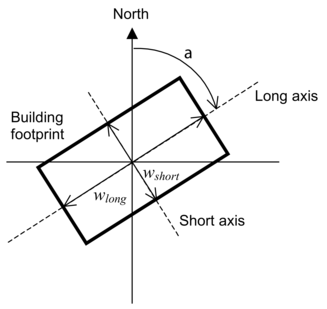
\includegraphics[width=0.9\textwidth, height=0.9\textheight, keepaspectratio=true]{media/image221.png}
\caption{Footprint of a rectangular building showing variables used by the program to calculate surface-average wind pressure coefficients. The angle a is the ``Azimuth Angle of Long Axis of Building.''  $w_{short}/w_{long}$ is the ``Ratio of Building Width Along Short Axis to Width Along Long Axis.'' \protect \label{fig:footprint-of-a-rectangular-building-showing}}
\end{figure}

\paragraph{Field: Height Dependence of External Node Temperature}\label{field-height-dependence-of-external-node-temperature}

This is an optional field. Input is Yes or No. The default is No. Yes is that external node temperature is dependent on node height. No means that external node temperature is calculated with zero height.

\paragraph{Field: Allow Unsupported Zone Equipment}\label{allow-unsupported-zone-equipment}

This is an optional field. Input is Yes or No. The default is No. Set this input to Yes to have zone equipment that are currently unsupported in the AirflowNetwork model allowed in the simulation. Setting this field to Yes, allows the following equipment to be modeled along an AirflowNetwork model: ZoneHVAC:Dehumidifier, ZoneHVAC:EnergyRecoveryVentilator, WaterHeater:HeatPump:*. The AirflowNetwork model will exclude mass balance in these equipment objects and assume the mass flows are self-balanced in the equipment objects.

An IDF example is shown below:

\begin{lstlisting}
AirflowNetwork:SimulationControl,
      AirflowNetwork_All,      !- Name
      MultiZoneWithDistribution,  !- AirflowNetwork Control
      Input,                   !- Wind Pressure Coefficient Type
      Every 30 Degrees,        !- AirflowNetwork Wind Pressure Coefficient Array Name
      OpeningHeight,           !- Height Selection for Local Wind Speed Calculation
      LowRise,                 !- Building Type
      500,                     !- Maximum Number of Iterations {dimensionless}
      ZeroNodePressures,       !- Initialization Type
      1.0E-05,                 !- Relative Airflow Convergence Tolerance {dimensionless}
      1.0E-06,                 !- Absolute Airflow Convergence Tolerance {kg/s}
      -0.5,                    !- Convergence Acceleration Limit {dimensionless}
      0.0,                     !- Azimuth Angle of Long Axis of Building {deg}
      1.0;                     !- Ratio of Building Width Along Short Axis to Width Along Long Axis
\end{lstlisting}

AirflowNetwork:MultiZone data objects are used to calculate multizone airflows. This section describes the input requirements for the following objects:

\begin{itemize}
\tightlist
\item
  \hyperref[airflownetworkmultizonezone]{AirflowNetwork:MultiZone:Zone}
\end{itemize}

AirflowNetwork:MultiZone data objects are used to calculate multizone airflows. This section describes the input requirements for the following objects:

\begin{itemize}
\item
  \hyperref[airflownetworkmultizonezone]{AirflowNetwork:MultiZone:Zone}
\item
  \hyperref[airflownetworkmultizonesurface]{AirflowNetwork:MultiZone:Surface}
\item
  \hyperref[airflownetworkmultizonesurfacecrack]{AirflowNetwork:MultiZone:Surface:Crack}
\item
  \hyperref[airflownetworkmultizonereferencecrackconditions]{AirflowNetwork:MultiZone:ReferenceCrackConditions}
\item
  \hyperref[airflownetworkmultizonesurfaceeffectiveleakagearea]{AirflowNetwork:MultiZone:Surface:EffectiveLeakageArea}
\item
  \hyperref[airflownetworkmultizonecomponentdetailedopening]{AirflowNetwork:MultiZone:Component:DetailedOpening}
\item
  \hyperref[airflownetworkmultizonecomponentsimpleopening]{AirflowNetwork:MultiZone:Component:SimpleOpening}
\item
  \hyperref[airflownetworkmultizonecomponenthorizontalopening]{AirflowNetwork:MultiZone:Component:HorizontalOpening}
\item
  \hyperref[airflownetworkmultizonecomponentzoneexhaustfan]{AirflowNetwork:MultiZone:Component:ZoneExhaustFan}
\item
  \hyperref[airflownetworkmultizoneexternalnode]{AirflowNetwork:MultiZone:ExternalNode}
\item
  \hyperref[airflownetworkmultizonewindpressurecoefficientarray]{AirflowNetwork:MultiZone:WindPressureCoefficientArray}
\item
  \hyperref[airflownetworkmultizonewindpressurecoefficientvalues]{AirflowNetwork:MultiZone:WindPressureCoefficientValues}
\end{itemize}

A detailed description for each of these objects is provided below.

\subsection{AirflowNetwork:MultiZone:Zone}\label{airflownetworkmultizonezone}

This object allows control of natural ventilation through exterior and interior openings in a zone, where ``opening'' is defined as an openable window or door. (Note that only window, door or glass door subsurfaces in a zone that are specified using \hyperref[airflownetworkmultizonecomponentdetailedopening]{AirflowNetwork:MultiZone:Component:DetailedOpening}, \hyperref[airflownetworkmultizonecomponenthorizontalopening]{AirflowNetwork:MultiZone:Component:HorizontalOpening} or \hyperref[airflownetworkmultizonecomponentsimpleopening]{AirflowNetwork:MultiZone:Component:SimpleOpening} and have an associated \hyperref[airflownetworkmultizonesurface]{AirflowNetwork:MultiZone:Surface} object are considered to be openings). The control will be applied in the same way to all of the openings in the zone.

This object is required to perform Airflow Network calculations. Note that ventilation control for all openings is provided at the zone level as default and individual ventilation control of a surface opening can be used to override the zone-level control (see the \hyperref[airflownetworkmultizonesurface]{AirflowNetwork:MultiZone:Surface} object description below).

\subsubsection{Field: Zone Name}\label{field-zone-name-001}

The name of the EnergyPlus thermal zone corresponding to the AirflowNetwork zone.

\subsubsection{Field: Ventilation Control Mode}\label{field-ventilation-control-mode}

Specifies the type of zone-level natural ventilation control.

Let T\(_{out}\) equal the outdoor air temperature, T\(_{zone}\) equal the previous timestep's zone air temperature, T\(_{set}\) equal the Vent Temperature Schedule value, H\(_{zone}\) equal the specific enthalpy of zone air from the previous timestep, and H\(_{out}\) equal the specific enthalpy of outdoor air. Then the four allowed choices for Ventilation Control Mode are:

\textbf{NoVent}: All of the zone's openable windows and doors are closed at all times independent of indoor or outdoor conditions. The Venting Availability Schedule is ignored in this case. This is the default value for this field.

\textbf{Temperature}: All of the zone's openable windows and doors are opened if T\(_{zone}\) \textgreater{} T\(_{out}\) \textbf{and} T\(_{zone}\) \textgreater{} T\(_{set}\) \textbf{and} Venting Availability Schedule (see below) allows venting.

\textbf{Enthalpy:} All of the zone's openable windows and doors are opened if H\(_{zone}\) \textgreater{} H\(_{out}\) \textbf{and} T\(_{zone}\) \textgreater{} T\(_{set}\) \textbf{and} Venting Availability Schedule allows venting.

\textbf{Constant}: Whenever this object's Venting Availability Schedule allows venting, all of the zone's openable windows and doors are open, independent of indoor or outdoor conditions. Note that ``Constant'' here means that the size of each opening is fixed while venting; the air flow through each opening can, of course, vary from timestep to timestep.

\textbf{ASHRAE55Adaptive}: All of the zone's operable windows and doors are opened if the operative temperature is greater than the comfort temperature (central line) calculated from the ASHRAE Standard 55-2010 adaptive comfort model and Venting Availability Schedule allows venting.

\textbf{CEN15251Adaptive:} All of the zone's operable windows and doors are opened if the operative temperature is greater than the comfort temperature (central line) calculated from the CEN15251 adaptive comfort model and Venting Availability Schedule allows venting.

\subsubsection{Field: Ventilation Control Zone Temperature Setpoint Schedule Name}\label{field-ventilation-control-zone-temperature-setpoint-schedule-name}

The name of a schedule of zone air temperature set points that controls the opening of windows and doors in the thermal zone to provide natural ventilation. This setpoint is the temperature above which all the openable windows and doors in the zone will be opened if the conditions described in the previous field Ventilation Control Mode are met.

The Ventilation Control Zone Temperature Setpoint Schedule Name applies only to windows and doors in the zone that are specified using \hyperref[airflownetworkmultizonecomponentdetailedopening]{AirflowNetwork:MultiZone:Component:DetailedOpening}, \hyperref[airflownetworkmultizonecomponenthorizontalopening]{AirflowNetwork:MultiZone:Component:HorizontalOpening} or \hyperref[airflownetworkmultizonecomponentsimpleopening]{AirflowNetwork:MultiZone:Component:SimpleOpening} and have an associated \hyperref[airflownetworkmultizonesurface]{AirflowNetwork:MultiZone:Surface} object.

(The discussion under the field Window/Door Opening Factor in the \hyperref[airflownetworkmultizonesurface]{AirflowNetwork:MultiZone:Surface} object describes how the actual opening area of a window or door in a particular timestep is determined.)

\emph{Modulation of Openings}

The following five fields can be used to modulate the window/door openings when Ventilation Control Mode = Temperature or Enthalpy. These fields determine a factor between 0 and 1 that multiplies the opening factor of each window and door in the zone according to the control action shown in Figure~\ref{fig:modulation-of-venting-area-according-to} for Ventilation Control Mode = Temperature and in Figure~\ref{fig:modulation-of-venting-area-according-to-001} for Ventilation Control Mode = Enthalpy. Modulation of the openings can reduce the large temperature swings that can occur if the windows/doors are open too far when they are venting, especially when there is a large inside-outside temperature difference.

The modulation takes the following form when Ventilation Control Mode = Temperature:

\textbf{if} T\(_{zone}\) - T\(_{out}\) ~\textless{} = ~ {[}Lower Value on Inside/Outside Temperature Difference for Modulating the Venting Open Factor{]}~~\textbf{then}~~Multiplication factor = 1.0

\textbf{if} {[}Lower Value on Inside/Outside Temperature Difference for Modulating the Venting Open Factor{]} \textless{} T\(_{zone}\) - T\(_{out}\) \textless{} {[}Upper Value on Inside/Outside Temperature Difference for Modulating the Venting Open Factor{]}~ \textbf{then} Multiplication factor varies linearly from 1.0 to {[}Limit Value on Multiplier for Modulating Venting Open Factor{]}

\textbf{if} T\(_{zone}\) - T\(_{out}\)~\textgreater{} = ~ {[}Upper Value on Inside/Outside Temperature Difference for Modulating the Venting Open Factor{]} \textbf{then} Multiplication factor = {[}Limit Value on Multiplier for Modulating Venting Open Factor{]}

One way of ``tuning'' the following modulation control parameters is to perform a sensitivity analysis for winter and/or summer design days to determine what combination of values causes the biggest reduction in zone air temperature fluctuations due to venting.

Note that the default values for the following fields are such that, if none of the fields are specified, the default values are assigned.

\subsubsection{Field: Minimum Venting Open Factor}\label{field-minimum-venting-open-factor}

See Figure~\ref{fig:modulation-of-venting-area-according-to} or Figure~\ref{fig:modulation-of-venting-area-according-to-001}. This field applies only if Ventilation Control Mode = Temperature or Enthalpy. This value may be from zero to 1.0, with the default being 0.0.

\subsubsection{Field: Indoor and Outdoor Temperature Difference Lower Limit For Maximum Venting Open Factor}\label{field-indoor-and-outdoor-temperature-difference-lower-limit-for-maximum-venting-open-factor}

See Figure~\ref{fig:modulation-of-venting-area-according-to}. This field applies only if Ventilation Control Mode = Temperature. This value may be from zero to less than \SI{100}{\celsius}, with the default being \SI{0}{\celsius}. The value for this field must be less than the value specified for the following field.

\subsubsection{Field: Indoor and Outdoor Temperature Difference Upper Limit for Minimun Venting Open Factor}\label{field-indoor-and-outdoor-temperature-difference-upper-limit-for-minimun-venting-open-factor}

See Figure~\ref{fig:modulation-of-venting-area-according-to}. This field applies only if Ventilation Control Mode = Temperature. This value must be greater than \SI{0}{\celsius}, with the default being \SI{100}{\celsius}. The value for this field must be greater than the value specified for the previous field..

\subsubsection{Field: Indoor and Outdoor Enthalpy Difference Lower Limit For Maximum Venting Open Factor}\label{field-indoor-and-outdoor-enthalpy-difference-lower-limit-for-maximum-venting-open-factor}

See Figure~\ref{fig:modulation-of-venting-area-according-to-001}. This field applies only if Ventilation Control Mode = Enthalpy. This value may be from zero to less than 300,000 J/kg, with the default being 0 J/kg. The value for this field must be less than the value specified for the following field.

\subsubsection{Field: Indoor and Outdoor Enthalpy Difference Upper Limit for Minimun Venting Open Factor}\label{field-indoor-and-outdoor-enthalpy-difference-upper-limit-for-minimun-venting-open-factor}

See Figure~\ref{fig:modulation-of-venting-area-according-to-001}. This field applies only if Ventilation Control Mode = Enthalpy. This value must be greater than zero, with the default being 300,000 J/kg. The value for this field must be greater than the value specified for the previous field.

\subsubsection{Field: Venting Availability Schedule Name}\label{field-venting-availability-schedule-name}

The name of a schedule that specifies when venting is available. A zero or negative schedule value means venting is not allowed. A value greater than zero means venting can occur if other venting control conditions (specified by Ventilation Control Mode and Vent Temperature Schedule Name) are satisfied. This schedule name should not be confused with Vent Temperature Schedule Name.

If a Venting Availability Schedule Name is not specified, it is assumed that venting is always available.

Using Venting Availability Schedule allows you to turn off venting at certain times of the day (at night, for example), of the week (on weekends, for example), or of the year (during the winter, for example).

If used with Ventilation Control Mode = Constant, the ventilation rate is constant only when this schedule allows venting; otherwise the ventilation rate is set to zero.

If Ventilation Control Mode = NoVent, this schedule has no effect.

\subsubsection{Field: Single Sided Wind Pressure Coefficient Algorithm}

Specifies the type of single sided wind pressure coefficient algorithm to be used for
the zone. This field is optional and is only used if Wind Pressure Coefficient Type is
set to SurfaceAverageCalculation. The default is Standard and the two valid choices are:

\textbf{Standard}: A single wind pressure coefficient is applied to all openings in the
zone, as calculated using SurfaceAverageCalculation.

\textbf{Advanced}: EnergyPlus calculates modified wind pressure coefficients for the two
openings in the zone. This model is only valid for zones with two openings, both of which
are on a single fa\c{c}ade (i.e. are coplanar). For zones with more than two openings,
consider combining the openings into two. The modified wind pressure coefficients account
for wind direction and turbulence effects on single sided ventilation rates. See the
Engineering Reference for a detailed description of the Advanced algorithm. When the
Advanced algorithm is selected, the difference between the two modified wind pressure
coefficients are output to the .eio file.

\subsubsection{Field: Fa\c{c}ade Width}
This is the whole building width along the direction of the facade of this zone, or
$W_F$ in Figure \ref{fig:single-sided-footprint}. This field is used in the Single
Sided Wind Pressure Coefficient Algorithm. This field is optional and is only used if
the Single Sided Wind Pressure Coefficient Algorithm is set to Advanced. The value must
be greater than 0.0 m, with the default being 10 m.

\begin{figure}[hbtp]
\centering
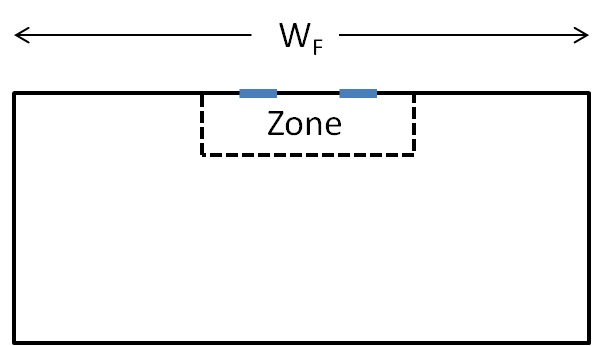
\includegraphics[width=0.9\textwidth, height=0.9\textheight, keepaspectratio=true]{media/single-sided-footprint.png}
\caption{Footprint of a rectangular building showing $W_F$, the ``Fa\c{c}ade Width'', used by the Single Sided Wind Pressure Coefficient Algorithm. \protect \label{fig:single-sided-footprint}}
\end{figure}

\subsubsection{Field: Occupant Ventilation Control Name}\label{field-occupant-ventilation-control-name}

The name of an AirlowNetwork:OccupantVentilationControl object. The object is used to perform advanced window opening control based on occupant conditions. When an object name is given, advanced window opening control is performed and, the ventilation control defined in the Ventilation Control Mode field will be overridden.

\textbf{Note:} The Occupant Ventilation Control object can be assigned to a zone (AirflowNetwork:MultiZone:Zone) or a surface (\hyperref[airflownetworkmultizonesurface]{AirflowNetwork:MultiZone:Surface}). When the object is assigned to a zone, the Occupant Ventilation Control is assigned to the surfaces belonging to the zone automatically. The surface objects must have an associated \hyperref[airflownetworkmultizonecomponentdetailedopening]{AirflowNetwork:MultiZone:Component:DetailedOpening}, \hyperref[airflownetworkmultizonecomponenthorizontalopening]{AirflowNetwork:MultiZone:Component:HorizontalOpening}, or \hyperref[airflownetworkmultizonecomponentsimpleopening]{AirflowNetwork:MultiZone:Component:SimpleOpening} component specified in the field of Leakage Component Name. All output variables will be shown under surface names only, and not under zone names.

\begin{figure}[hbtp] % fig 96
\centering
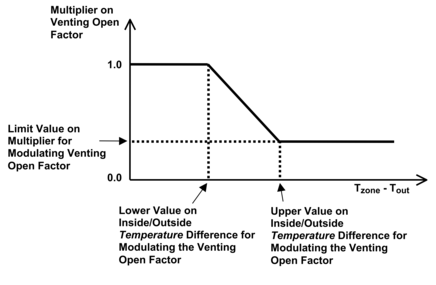
\includegraphics[width=0.9\textwidth, height=0.9\textheight, keepaspectratio=true]{media/image222.png}
\caption{Modulation of venting area according to inside-outside temperature difference. \protect \label{fig:modulation-of-venting-area-according-to}}
\end{figure}

\begin{figure}[hbtp] % fig 97
\centering
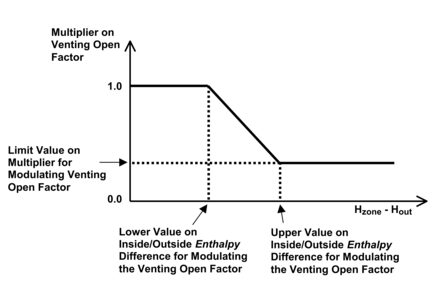
\includegraphics[width=0.9\textwidth, height=0.9\textheight, keepaspectratio=true]{media/image223.png}
\caption{Modulation of venting area according to inside-outside enthalpy difference. \protect \label{fig:modulation-of-venting-area-according-to-001}}
\end{figure}

\textbf{Note:} In order to establish an airflow network, each AirflowNetwork:MultiZone:Zone object must have at least two surfaces defined with \hyperref[airflownetworkmultizonesurface]{AirflowNetwork:MultiZone:Surface} objects, so that air can flow from one zone into other zones (or to outdoors) through the network (air mass flow conserved). In addition, for all \hyperref[airflownetworkmultizonesurface]{AirflowNetwork:MultiZone:Surface} objects facing the same Zone (ref. \hyperref[buildingsurfacedetailed]{BuildingSurface:Detailed}), at least two different environments must be defined for the other side of these surfaces (e.g., an external node and an adjacent zone, two adjacent zones, or two external nodes).

An IDF example is shown below:

\begin{lstlisting}
AirflowNetwork:MultiZone:Zone,
      RESISTIVE ZONE,          !- Name of Associated Thermal Zone
      Temperature,             !- Ventilation Control Mode
      WindowVentSched,         !- Vent Temperature Schedule Name
      0.3,                     !- Limit Value on Multiplier for Modulating Venting Open Factor
                               !- {dimensionless}
      5.0,                     !- Lower Value on Inside/Outside Temperature Difference for
                               !- Modulating the Venting Open Factor {deltaC}
      10.0,                    !- Upper Value on Inside/Outside Temperature Difference for
                               !- Modulating the Venting Open Factor {deltaC}
      0.0,                     !- Lower Value on Inside/Outside Enthalpy Difference for Modulating
                               !- the Venting Open Factor {J/kg}
      300000.0,                !- Upper Value on Inside/Outside Enthalpy Difference for Modulating
                               !- the Venting Open Factor {J/kg}
      VentingSched;            !- Venting Availability Schedule Name
\end{lstlisting}

\subsection{AirflowNetwork:MultiZone:Surface}\label{airflownetworkmultizonesurface}

The AirflowNetwork:MultiZone:Surface object specifies the properties of a surface ``linkage'' through which air flows. This linkage is always associated with a building surface (wall, roof, floor, or a ceiling) or subsurface (door, glass door, or window) with both faces exposed to air. The linkage specifies two connected nodes: two zone nodes defined in \hyperref[airflownetworkmultizonezone]{AirflowNetwork:MultiZone:Zone} objects based on inside and outside face environment for an interior surface, or a zone node defined in an \hyperref[airflownetworkmultizonezone]{AirflowNetwork:MultiZone:Zone} object based on inside face environment and an external node defined in an \hyperref[airflownetworkmultizoneexternalnode]{AirflowNetwork:MultiZone:ExternalNode} object for an exterior surface. The associated leakage component for this surface can be a crack (or surface effective leakage area) in an exterior or interior heat transfer surface or subsurface, or an exterior or interior window, door or glass door (heat transfer subsurface) that can be opened to allow air flow. The allowed surface air leakage components are:

\begin{itemize}
\item
  \hyperref[airflownetworkmultizonesurfacecrack]{AirflowNetwork:MultiZone:Surface:Crack}
\item
  \hyperref[airflownetworkmultizonesurfaceeffectiveleakagearea]{AirflowNetwork:MultiZone:Surface:EffectiveLeakageArea}
\item
  \hyperref[airflownetworkmultizonecomponentdetailedopening]{AirflowNetwork:MultiZone:Component:DetailedOpening}
\item
  \hyperref[airflownetworkmultizonecomponenthorizontalopening]{AirflowNetwork:MultiZone:Component:HorizontalOpening}
\item
  \hyperref[airflownetworkmultizonecomponentsimpleopening]{AirflowNetwork:MultiZone:Component:SimpleOpening}
\item
  \hyperref[airflownetworkmultizonecomponentzoneexhaustfan]{AirflowNetwork:MultiZone:Component:ZoneExhaustFan}
\end{itemize}

The three ``opening'' components are used to modulate openness based on required conditions.

The AirflowNetwork:MultiZone:Surface object allows a heat transfer surface or subsurface to have one crack (or one surface effective leakage area object), or a subsurface (i.e., window, door or glass door) to have one opening (detailed, simple, or horizontal).


An interior heat transfer surface (\hyperref[buildingsurfacedetailed]{BuildingSurface:Detailed}) whose surface name is used as the input for the Outside Boundary Condition Object field is adiabatic and is not allowed as an AirflowNetwork:MultiZone:Surface. A heat transfer surface defined in the BuildingSurface:Detailed:ExteriorNaturalVentedCavity is also not allowed.

When a non-rectangular subsurface is used, the model will automatically convert it into a rectangular subsurface using equivalent width and height based on an entered choice from the Equivalent Rectangle Method field or a default choice.

When an air boundary surface or subsurface is used (\hyperref[constructionairboundary]{Construction:AirBoundary}), all types of leakage component are allowed except AirflowNetwork:MultiZone:Component:ZoneExhaustFan. The only allowed venting control type for an air boundary surface is Constant, and the venting schedule is ignored (which means the opening is always fully open at the specified Window/Door Opening Factor, or Crack Factor). EnergyManagementSystem:Actuator ``AirFlow Network Window/Door Opening'' is available for special applications where control of the air boundary opening is required.

\subsubsection{Field: Surface Name}\label{field-surface-name-000}

This is the name of the corresponding surface (wall, roof, ceiling, floor, window, door or glass door).

Information on this surface is used by the program as follows:

\begin{itemize}
\item
For a linkage associated with an exterior heat transfer surface: air flow through this linkage is between the outside environment and the thermal zone to which the surface belongs.

\item
For a linkage associated with an interior (i.e., interzone) heat transfer surface: air flow through this linkage is between the thermal zones separated by the surface (i.e., the thermal zone associated with the inside face environment and the thermal zone associated with the outside face environment).

\item
This heat transfer surface determines the height of the linkage, which is used in calculating buoyancy-related flow through the linkage.

\item
The surface may be an air boundary surface or subsurface (\hyperref[constructionairboundary]{Construction:AirBoundary}).
\end{itemize}

\textbf{Note:} It is possible to define an interzone surface twice in EnergyPlus, once in each of the zones that the surface separates. Previously this was a requirement of EnergyPlus (prior to version 2.0), but now it is optional and the user also has the option of only defining the surface once (EnergyPlus defines the second surface automatically within the program). For each interzone surface, use only one (of possible two) interzone surface names in the AirflowNetwork:MultiZone:Surface object for ``Surface Name.'' \textbf{Do not} enter two AirflowNetwork:MultiZone:Surface objects corresponding to the two possible interzone names. This would cause the air flow through the surface to be counted twice.

\subsubsection{Field: Leakage Component Name}\label{field-leakage-component-name}

The name of the \hyperref[airflownetworkmultizonesurfacecrack]{AirflowNetwork:MultiZone:Surface:Crack}, \hyperref[airflownetworkmultizonesurfaceeffectiveleakagearea]{AirflowNetwork:MultiZone:Surface:EffectiveLeakageArea}, \hyperref[airflownetworkmultizonecomponentsimpleopening]{AirflowNetwork:MultiZone:Component:SimpleOpening}, \hyperref[airflownetworkmultizonecomponenthorizontalopening]{AirflowNetwork:MultiZone:Component:HorizontalOpening}, \hyperref[airflownetworkmultizonecomponentdetailedopening]{AirflowNetwork:MultiZone:Component:DetailedOpening} or \hyperref[airflownetworkmultizonecomponentzoneexhaustfan]{AirflowNetwork:MultiZone:Component:ZoneExhaustFan} object associated with this air flow linkage.

If the name of an opening component (i.e.~\hyperref[airflownetworkmultizonecomponentdetailedopening]{AirflowNetwork:MultiZone:Component:DetailedOpening}. \hyperref[airflownetworkmultizonecomponenthorizontalopening]{AirflowNetwork:MultiZone:Component:HorizontalOpening},~ or \hyperref[airflownetworkmultizonecomponentsimpleopening]{AirflowNetwork:MultiZone:Component:SimpleOpening} is given here, then the Surface Name in the previous field must be that of a window, door or glass door heat transfer subsurface or a building surface which is an air boundary. Otherwise an error message will be reported.

If the name of an \hyperref[airflownetworkmultizonesurfacecrack]{AirflowNetwork:MultiZone:Surface:Crack} object or \hyperref[airflownetworkmultizonesurfaceeffectiveleakagearea]{AirflowNetwork:MultiZone:Surface:EffectiveLeakageArea} object is given here, the program will position the crack at the average height of the associated heat transfer surface or subsurface. The user can define multiple heat transfer surfaces (e.g., split a wall into several surfaces) to be more precise in establishing the crack location. Similarly, the user can define multiple heat transfer surfaces if a wall, for example, has multiple cracks or openings that need to be defined individually.

If the name of an \hyperref[airflownetworkmultizonecomponentzoneexhaustfan]{AirflowNetwork:MultiZone:Component:ZoneExhaustFan} is given here, then the Surface Name in the previous field must be that of an exterior heat transfer surface. The zone name defined in the Zone Name field for this heat transfer surface must be the same zone name defined in the \hyperref[zonehvacequipmentconnections]{ZoneHVAC:EquipmentConnections} object (which references a \hyperref[zonehvacequipmentlist]{ZoneHVAC:EquipmentList} containing the name of the corresponding zone exhaust fan).Otherwise an error message will be reported. When this zone exhaust fan is operating for a simulation timestep, all surface-level controls described below are ignored for that timestep.

\subsubsection{Field: External Node Name}\label{field-external-node-name}

The name of the associated \hyperref[airflownetworkmultizoneexternalnode]{AirflowNetwork:MultiZone:ExternalNode} object, which
determines the wind pressure coefficients for the heat transfer surface. Used
only if Surface Name is for an exterior surface.

If Wind Pressure Coefficient Type = SurfaceAverageCalculation in the \hyperref[airflownetworksimulationcontrol]{AirflowNetwork:\hyperref[simulationcontrol]{SimulationControl}}
object, this field is not used and a blank may be entered. If the surface is an
interior (i.e., interzone) surface, leave this field blank.

When there is an input object of either \hyperref[ZonePropertylocalEnvironment]{ZoneProperty:LocalEnvironment} or \hyperref[surfacePropertylocalEnvironment]{SurfaceProperty:LocalEnvironment}, LocalEnvironment is enable, so that entered names of \hyperref[outdoorairnode]{OutdoorAir:Node} can be used as inputs for this field. More descrption of use can be found in  OutdoorAir:Node.

\subsubsection{Field: Window/Door Opening Factor, or Crack Factor}\label{field-windowdoor-opening-factor-or-crack-factor}

If this linkage is associated with an \hyperref[airflownetworkmultizonecomponentdetailedopening]{AirflowNetwork:MultiZone:Component:DetailedOpening} or \hyperref[airflownetworkmultizonecomponentsimpleopening]{AirflowNetwork:MultiZone:Component:SimpleOpening} object (which means it is an openable window or door), then this field is called ``Window/Door Opening Factor'' and represents the value of the Opening Factor that is in effect when the Vent Temperature Schedule (defined in the \hyperref[airflownetworkmultizonezone]{AirflowNetwork:MultiZone:Zone} object) indicates that this window or door is open.

The AirflowNetwork model uses a combination of factors to determine the actual opening area for a window or door when it is venting. For example, consider a window that is 1.5m high and 2.0m wide (excluding frame). Assume that the \hyperref[airflownetworkmultizonecomponentdetailedopening]{AirflowNetwork:MultiZone:Component:DetailedOpening} for this window has Type of Large Vertical Opening = 1 (non-pivoting window), Height Factor = 0.5 and Width Factor = 0.8. Then when the window is fully open, the opening area = height of opening (0.5x1.5) times width of opening (0.8x2.0) = 0.75x1.6 = 1.2 m\(^{2}\). If the Window/Door Opening Factor is 0.75, then the opening area = 0.75x1.2 = 0.9 m\(^{2}\).

If, in addition, the window is in a thermal zone for which opening modulation has been specified (ref: \hyperref[airflownetworkmultizonezone]{AirflowNetwork:MultiZone:Zone}) and the multiplication factor due to modulation is 0.3 in a particular timestep, then the actual opening factor that timestep = 0.3x0.75 = 0.225 and the actual opening area that timestep = 0.3x0.9 = 0.27 m\(^{2}\).

If this linkage is associated with an \hyperref[airflownetworkmultizonesurfacecrack]{AirflowNetwork:MultiZone:Surface:Crack} object, the following crack air flow equation is used.

\begin{equation}
Q = \left( Crack\;Factor \right) * C_T * C_Q \left( \Delta P \right)^{n}
\end{equation}

Where

$Q$ is the air mass flow (kg/s)

$C_Q$ is the air mass flow coefficient (kg/s @ 1 Pa)

$C_T$ is the reference condition temperature correction factor (dimensionless). See \hyperref[airflownetworkmultizonesurfacecrack]{AirflowNetwork:MultiZone:Surface:Crack} object.

$\Delta P$ is the pressure difference across crack (Pa)

$n$ is the air flow exponent (dimensionless)

\emph{The following fields control venting. They are used only when Name of Associated Heat Transfer Surface is that of an openable exterior or interior window, door or glass door. They only apply to openings, and do not apply to surface cracks, effective leakage area or zone exhaust fans. If none of these fields is specified, or if Ventilation Control Mode = ZoneLevel, venting is controlled by the \hyperref[airflownetworkmultizonezone]{AirflowNetwork:MultiZone:Zone} object for the thermal zone containing the window or door (ref: \hyperref[airflownetworkmultizonezone]{AirflowNetwork:MultiZone:Zone} Data).}

\subsubsection{Field: Ventilation Control Mode}\label{field-ventilation-control-mode-1}

Specifies the type of surface-level natural ventilation control.

Let $T_{out}$ equals the outdoor air temperature, $T_{zone}$ equals the previous
timestep's zone air temperature, $T_{set}$ equals the Vent Temperature Schedule
value, $H_{zone}$ equals the specific enthalpy of zone air from the previous
timestep, and $H_{out}$ equals the specific enthalpy of outdoor air. Then the
four allowed choices for Ventilation Control Mode are:

\textbf{NoVent}: The openable window or door associated with this surface is
closed at all times independent of indoor or outdoor conditions. The
Venting Availability Schedule is ignored in this case.

\textbf{Temperature}: The openable window or door associated with this surface
is opened if $T_{zone} > T_{out}$ \textbf{and} $T_{zone} > T_{set}$ \textbf{and}
Venting Availability Schedule (see below) allows venting.

\textbf{Enthalpy:} The openable window or door associated with this surface is
opened if $H_{zone} > H_{out}$ \textbf{and} $T_{zone} > T_{set}$ \textbf{and}
Venting Availability Schedule allows venting.

\textbf{Constant}: Whenever this object's Venting Availability Schedule allows venting, the openable window or door associated with this surface is open, independent of indoor or outdoor conditions. Note that ``Constant'' here means that the size of this opening is fixed while venting; the air flow through this opening can, of course, vary from timestep to timestep. If the surface is an air boundary (\hyperref[constructionairboundary]{Construction:AirBoundary}) then Constant is the only valid option (other options will throw a warning and be reset to Constant).

\textbf{ASHRAE55Adaptive}: The openable window or door associated with this surface is opened if the operative temperature is greater than the comfort temperature (central line) calculated from the ASHRAE Standard 55-2010 adaptive comfort model \textbf{and} Venting Availability Schedule allows venting.

\textbf{CEN15251Adaptive:} The openable window or door associated with this surface is opened if the operative temperature is greater than the comfort temperature (central line) calculated from the CEN15251 adaptive comfort model \textbf{and} Venting Availability Schedule allows venting.

\textbf{ZoneLevel}: Venting of the window or door is not controlled individually, but is controlled instead at the zone level. This means that the venting is determined by the \hyperref[airflownetworkmultizonezone]{AirflowNetwork:MultiZone:Zone} object for the thermal zone containing the window or door (ref: \hyperref[airflownetworkmultizonezone]{AirflowNetwork:MultiZone:Zone} object). This is the default value for this field.

\textbf{AdjacentTemperature}: This choice is used for an interior surface only.
The openable interior window or door associated with this surface is opened if
$T_{zone} > T_{adjacent\ zone}$ \textbf{and} $T_{zone} > T_{set}$ \textbf{and}
Venting Availability Schedule (see below) allows venting, where $T_{adjacent\ zone}$
is the adjacent zone temperature.

\textbf{AdjacentEnthalpy:} This choice is also used for an interior surface only.
The interior openable window or door associated with this surface is opened if
$H_{zone} > H_{adjacent\ zone}$ \textbf{and} $T_{zone} > T_{set}$ \textbf{and}
Venting Availability Schedule allows venting, where $H_{adjacent\ zone}$ is the
adjacent zone specific enthalpy.

\subsubsection{Field: Ventilation Control Zone Temperature Setpoint Schedule Name}\label{field-ventilation-control-zone-temperature-setpoint-schedule-name-1}

The name of a schedule of zone air temperature set points that controls the opening of a window or door associated with this surface to provide natural ventilation. This setpoint is the temperature above which this openable window or door will be opened if the conditions described in the previous field Ventilation Control Mode are met.

The Ventilation Control Zone Temperature Setpoint Schedule applies only to a window or door attached to this surface that is specified using \hyperref[airflownetworkmultizonecomponentdetailedopening]{AirflowNetwork:MultiZone:Component:DetailedOpening} or \hyperref[airflownetworkmultizonecomponentsimpleopening]{AirflowNetwork:MultiZone:Component:SimpleOpening}.

(The discussion under the field Window/Door Opening Factor in this object describes how the actual opening area of a window or door in a particular timestep is determined.)

\emph{Modulation of Openings}

The following five fields can be used to modulate this window/door opening when Ventilation Control Mode = Temperature or Enthalpy. These fields determine a factor between 0 and 1 that multiplies the opening factor of this window or door according to the control action shown in Figure~\ref{fig:modulation-of-venting-area-according-to} for Ventilation Control Mode = Temperature and in Figure~\ref{fig:modulation-of-venting-area-according-to-001} for Ventilation Control Mode = Enthalpy. Modulation of this opening can reduce the large temperature swings that can occur if the window/door is open too far when it is venting, especially when there is a large inside-outside temperature difference.

The modulation takes the following form when Ventilation Control Mode = Temperature:

\textbf{if} T\(_{zone}\) - T\(_{out}\)~\textless{} = {[}Lower Value on Inside/Outside Temperature Difference for Modulating the Venting Open Factor{]}~~\textbf{then}~~Multiplication factor = 1.0

\textbf{if} {[}Lower Value on Inside/Outside Temperature Difference for Modulating the Venting Open Factor{]} \textless{} T\(_{zone}\) - T\(_{out}\) \textless{} {[}Upper Value on Inside/Outside Temperature Difference for Modulating the Venting Open Factor{]}~ \textbf{then} Multiplication factor varies linearly from 1.0 to {[}Limit Value on Multiplier for Modulating Venting Open Factor{]}

\textbf{if} T\(_{zone}\) - T\(_{out}\)~\textgreater{} = ~ {[}Upper Value on Inside/Outside Temperature Difference for Modulating the Venting Open Factor{]}~ \textbf{then} Multiplication factor = {[}Limit Value on Multiplier for Modulating Venting Open Factor{]}

One way of ``tuning'' the following modulation control parameters is to perform a sensitivity analysis for winter and/or summer design days to determine what combination of values causes the biggest reduction in zone air temperature fluctuations due to venting.

Note that the default values for the following fields are such that, if none of the fields are specified, modulation will not occur.

\subsubsection{Field: Minimum Venting Open Factor}\label{field-minimum-venting-open-factor-1}

See Figure~\ref{fig:modulation-of-venting-area-according-to} or Figure~\ref{fig:modulation-of-venting-area-according-to-001}. This field applies only if Ventilation Control Mode = Temperature or Enthalpy. This value may be from zero to 1.0, with the default being 0.0.

\subsubsection{Field: Indoor and Outdoor Temperature Difference Lower Limit For Maximum Venting Open Factor}\label{field-indoor-and-outdoor-temperature-difference-lower-limit-for-maximum-venting-open-factor-1}

See Figure~\ref{fig:modulation-of-venting-area-according-to}. This field applies only if Ventilation Control Mode = Temperature. This value may be from zero to less than 100°C, with the default being 0°C. The value for this field must be less than the value specified for the following field.

\subsubsection{Field: Indoor and Outdoor Temperature Difference Upper Limit for Minimun Venting Open Factor}\label{field-indoor-and-outdoor-temperature-difference-upper-limit-for-minimun-venting-open-factor-1}

See Figure~\ref{fig:modulation-of-venting-area-according-to}. This field applies only if Ventilation Control Mode = Temperature. This value must be greater than 0°C, with the default being 100°C. The value for this field must be greater than the value specified for the previous field.

\subsubsection{Field: Indoor and Outdoor Enthalpy Difference Lower Limit For Maximum Venting Open Factor}\label{field-indoor-and-outdoor-enthalpy-difference-lower-limit-for-maximum-venting-open-factor-1}

See Figure~\ref{fig:modulation-of-venting-area-according-to-001}. This field applies only if Ventilation Control Mode = Enthalpy. This value may be from zero to less than 300,000 J/kg, with the default being 0 J/kg. The value for this field must be less than the value specified for the following field.

\subsubsection{Field: Indoor and Outdoor Enthalpy Difference Upper Limit for Minimun Venting Open Factor}\label{field-indoor-and-outdoor-enthalpy-difference-upper-limit-for-minimun-venting-open-factor-1}

See Figure~\ref{fig:modulation-of-venting-area-according-to-001}. This field applies only if Ventilation Control Mode = Enthalpy. This value must be greater than zero, with the default being 300,000 J/kg. The value for this field must be greater than the value specified for the previous field.

\subsubsection{Field: Venting Availability Schedule Name}\label{field-venting-availability-schedule-name-1}

The name of a schedule that specifies when venting is available. A zero or negative schedule value means venting is not allowed. A value greater than zero means venting can occur if other venting control conditions (specified by Ventilation Control Mode and Vent Temperature Schedule Name) are satisfied. This schedule name should not be confused with Vent Temperature Schedule Name.  If the surface is an air boundary (\hyperref[constructionairboundary]{Construction:AirBoundary}) then this field is ignored and venting is always available.

If a Venting Availability Schedule Name is not specified, it is assumed that venting is always available.

Using Venting Availability Schedule allows you to turn off venting at certain times of the day (at night, for example), week (on weekends, for example), or year (during the winter, for example).

If used with Ventilation Control Mode = Constant, the ventilation rate is constant only when this schedule allows venting; otherwise the ventilation rate is set to zero.

If Ventilation Control Mode = NoVent, this schedule has no effect.

\textbf{Note:} In order to establish an airflow network, each \hyperref[airflownetworkmultizonezone]{AirflowNetwork:MultiZone:Zone} object must have at least two surfaces defined with AirflowNetwork:MultiZone:Surface objects, so that air can flow from one zone into other zones (or to outdoors) through the network (air mass flow conserved). In addition, for all AirflowNetwork:MultiZone:Surface objects facing the same Zone Name (ref. \hyperref[buildingsurfacedetailed]{BuildingSurface:Detailed}), at least two different environments must be defined for the other side of these surfaces (e.g., an external node and an adjacent zone, two adjacent zones, or two external nodes).

\subsubsection{Field: Occupant Ventilation Control Name}\label{field-occupant-ventilation-control-name-1}

The name of an AirlowNetwork:OccupantVentilationControl object. The object is used to perform advanced window opening control based on occupant conditions. When an object name is given, advanced window opening control is performed and, the Ventilation Control defined in the Ventilation Control Mode field will be overridden.

\subsubsection{Field: Equivalent Rectangle Method }\label{equivalent-rectangle-method}

This field is applied to a non-rectangular window or door. The equivalent
rectangular surface has the same area as the non-rectangular one. The valid
choices are: PolygonHeight, BaseSurfaceAspectRatio, and UserDefinedAspectRatio,
with the default of PolygonHeight. When PolygonHeight is entered, the equivalent
width is equal to the area divided by the PolygonHeight for a non-horizontal
surface. When a surface is horizontal with the same height for all vertices,
the model will automatically switch a choice to BaseSurfaceAspectRatio if a
base surface is rectangular, or UserDefinedAspectRatio with the default value if
a base surface is non-rectangular.  When BaseSurfaceAspectRatio is entered for
a rectangular base surface, the equivalent height is equal to Square Root of
Area divided by the base surface aspect ratio. The equivalent width is equal
to the equivalent height times the base surface aspect ratio. When a base
surface is non-rectangular, the model will automatically switch the choice to
PolygonHeight for a non-horizontal base surface, and UserDefinedAspectRatio
with the default value if a base surface is horizontal. When
UserDefinedAspectRatio is entered, the equivalent height is equal to Square
Root of Area divided by UserDefinedAspectRatio. The equivalent width is equal
to the equivalent height times the user-defined aspect ratio.

 \subsubsection{Field: Equivalent Rectangle Aspect Ratio}\label{equivalent-rectangular-aspect-ratio}

 This field applies only if Equivalent Rectangle Method = UserDefinedAspectRatio. This value must be greater than zero, with the default being 1.0.

IDF examples are provided below:

\begin{lstlisting}
AirflowNetwork:MultiZone:Surface,
      Zn001:Wall001,           !- Name of Associated Heat Transfer Surface
      CR-1,                    !- Leakage Component Name
      SFacade,                 !- External Node Name
      1.0;                     !- Window/Door Opening Factor, or Crack Factor {dimensionless}

  AirflowNetwork:MultiZone:Surface,
      Zn001:Wall001:Win001,    !- Name of Associated Heat Transfer Surface
      WiOpen1,                 !- Leakage Component Name
      SFacade,                 !- External Node Name
      0.5;                     !- Window/Door Opening Factor, or Crack Factor {dimensionless}

  AirflowNetwork:MultiZone:Surface,
      Zn003:Wall003,           !- Name of Associated Heat Transfer Surface
      Zone3 Exhaust Fan,       !- Leakage Component Name
      EFacade,                 !- External Node Name
      1.0;                     !- Window/Door Opening Factor, or Crack Factor {dimensionless}

  AirflowNetwork:MultiZone:Surface,
      Zn001:Wall001:Win002,    !- Name of Associated Heat Transfer Surface
      WiOpen2,                 !- Leakage Component Name
      WFacade,                 !- External Node Name
      0.5;                     !- Window/Door Opening Factor, or Crack Factor {dimensionless}
      Temperature,             !- Ventilation Control Mode
      WindowVentSched,         !- Vent Temperature Schedule Name
      0.3,                     !- Limit Value on Multiplier for Modulating Venting Open Factor
                               !- {dimensionless}
      5.0,                     !- Lower Value on Inside/Outside Temperature Difference for
                               !- Modulating the Venting Open Factor {deltaC}
      10.0,                    !- Upper Value on Inside/Outside Temperature Difference for
                               !- Modulating the Venting Open Factor {deltaC}
      0.0,                     !- Lower Value on Inside/Outside Enthalpy Difference for Modulating
                               !- the Venting Open Factor {J/kg}
      300000.0,                !- Upper Value on Inside/Outside Enthalpy Difference for Modulating
                               !- the Venting Open Factor {J/kg}
      VentingSched;            !- Venting Availability Schedule Name
\end{lstlisting}

\subsection{AirflowNetwork:MultiZone:ReferenceCrackConditions}\label{airflownetworkmultizonereferencecrackconditions}

This object specifies the reference conditions for temperature, humidity, and pressure which correspond to the \hyperref[airflownetworkmultizonesurfacecrack]{AirflowNetwork:MultiZone:Surface:Crack} object.

\subsubsection{Inputs}\label{inputs-1-004}

\paragraph{Field: Name}\label{field-name-1-003}

The name of this Reference Crack Conditons object. This name is referenced by an \hyperref[airflownetworkmultizonesurfacecrack]{AirflowNetwork:MultiZone:Surface:Crack} object.

\paragraph{Field: Reference Temperature}\label{field-reference-temperature}

The reference temperature in °C under which the Surface Crack Data were obtained. The default value is 20°C.

\paragraph{Field: Reference Barometric Pressure}\label{field-reference-barometric-pressure}

The reference barometric pressure in Pa under which the Surface Crack Data were obtained. The default value is 101325 Pa.

\paragraph{Field: Reference Humidity Ratio}\label{field-reference-humidity-ratio}

The reference humidity ratio in kgWater/kgDryAir under which the Surface Crack Data were obtained. The default value is 0 kgWater/kgDryAir.

An IDF example is provided below:

\begin{lstlisting}
AirflowNetwork:MultiZone:ReferenceCrackConditions,
      ReferenceCrackConditions,      !- Name of Reference Crack Conditions
      20.0,                          !- Reference Temperature for Crack Data {C}
      101325,                        !- Reference Barometric Pressure for Crack Data {Pa}
      0.0;                           !- Reference Humidity Ratio for Crack Data {kgWater/kgDryAir}
\end{lstlisting}

\subsection{AirflowNetwork:MultiZone:Surface:Crack}\label{airflownetworkmultizonesurfacecrack}

This object specifies the properties of air flow through a crack and the associated measurement conditions. The following power law form is used that gives air flow through the crack as a function of the pressure difference across the crack:

\begin{equation}
Q = \left( Crack\;Factor \right) * C_T * C_Q \left( \Delta P \right)^{n}
\end{equation}

Where

\emph{Q}~~~ = air mass flow (kg/s)

\emph{C\(_{Q}\)}~ = air mass flow coefficient (kg/s-Pa\(^{n}\) @ 1 Pa)

\emph{C\(_{T}\)}~ = reference condition temperature correction factor (dimensionless)

\(\Delta P\) = pressure difference across crack (Pa)

\emph{n}~~~ = air flow exponent (dimensionless)

\begin{equation}
{C_T} = {\left[ {\frac{{{\rho_o}}}{\rho }} \right]^{n - 1}}{\left[ {\frac{{{\nu_o}}}{\nu }} \right]^{2n - 1}}
\end{equation}

where

\(\rho\) = Air density at the specific air temperature and humidity ratio conditions {[}kg/m\(^{3}\){]}

\(\nu\) = Air kinetic viscosity at the specific air temperature condition {[}m\(^{2}\)/s{]}

\(\rho_o\) = Air density at the reference air conditions provided by the object Air\-flow\-Net\-work:\-Multi\-Zone:\-Refer\-ence\-Crack\-Con\-ditions specified in the field Reference Crack Conditions {[}kg/m\(^{3}\){]}

\(\nu_o\) = Air kinetic viscosity at the reference air temperature provided by the object Air\-flow\-Net\-work:\-Multi\-Zone:\-Refer\-ence\-Crack\-Con\-ditions specified in the field Reference Crack Conditions {[}m\(^{2}\)/s{]}

Note: The correction factor shown above is use for this particular component as specified.

\subsubsection{Inputs}\label{inputs-2-004}

\paragraph{Field: Name}\label{field-name-2-003}

This is a name for this AirflowNetwork:MultiZone:Surface:Crack object. It is referenced by an \hyperref[airflownetworkmultizonesurface]{AirflowNetwork:MultiZone:Surface} object.

\paragraph{Field: Air Mass Flow Coefficient at Reference Conditions}\label{field-air-mass-flow-coefficient-at-reference-conditions}

The value of the air mass flow coefficient,\({C_Q}\) , in the crack air flow equation. It has units of kg/s at 1Pa. This value must be greater than zero.

\paragraph{Field: Air Mass Flow Exponent}\label{field-air-mass-flow-exponent}

The value of the exponent, \emph{n}, in the crack air flow equation. The valid range is 0.5 to 1.0, with the default value being 0.65.

\paragraph{Field: Reference Crack Conditions}\label{field-reference-crack-conditions}

The name of the \hyperref[airflownetworkmultizonereferencecrackconditions]{AirflowNetwork:MultiZone:ReferenceCrackConditions} object which specifies the conditions under which the air mass flow coefficient was measured. If the user omits this field and only one \hyperref[airflownetworkmultizonereferencecrackconditions]{AirflowNetwork:MultiZone:ReferenceCrackConditions} object is defined in the input data file, then those reference crack conditions will be used. If the user omits this field and either zero or more than one \hyperref[airflownetworkmultizonereferencecrackconditions]{AirflowNetwork:MultiZone:ReferenceCrackConditions} objects are defined in the input data file, then the default conditions for the AirflowNetwork:MultiZone: Reference Crack Conditions object will be used.

An IDF example is shown below:

\begin{lstlisting}
AirflowNetwork:MultiZone:Surface:Crack,
  CR-1,                   !- Name of Surface Crack Component
  0.01,                   !- Air Mass Flow Coefficient at Reference Conditions {kg/s}
  0.667,                  !- Air Mass Flow Exponent {dimensionless}
  ReferenceCrackConditions; !- Reference Crack Conditions
\end{lstlisting}

\subsection{AirflowNetwork:MultiZone:Surface:EffectiveLeakageArea}\label{airflownetworkmultizonesurfaceeffectiveleakagearea}

The effective leakage area (ELA) object is used to define surface air leakage. It has

five fields. The relationship between pressure and airflow may be expressed as:

\begin{equation}
\dot m = ELA*{C_d}\sqrt {2\rho } *{\left( {\Delta {P_r}} \right)^{0.5 - n}}{\left( {\Delta P} \right)^n}
\end{equation}

where

\(\dot m\) = Air mass flow rate {[}kg/s{]}

\(\rm{ELA}\) = Effective leakage area {[}m\(^{2}\){]}

\(\rho\) = Air density {[}kg/m\(^{3}\){]}

\(\Delta {P_r}\) = Reference pressure difference {[}Pa{]}

\(\Delta P\) = Pressure difference across this component {[}Pa{]}

\(C_{d}\) = Discharge coefficient {[}dimensionless{]}

\(n\) = Air mass flow exponent {[}dimensionless{]}

\subsubsection{Inputs}\label{inputs-3-003}

\paragraph{Field: Name}\label{field-name-3-003}

This is a name for this AirflowNetwork:MultiZone:Surface:EffectiveLeakageArea object. It is referenced by an \hyperref[airflownetworkmultizonesurface]{AirflowNetwork:MultiZone:Surface} object.

\paragraph{Field: Effective Leakage Area}\label{field-effective-leakage-area}

This numeric field is used to input the effective leakage area~ in square meters. The effective leakage area is used to characterize openings for infiltration calculations (ASHRAE Handbook of Fundamentals, 1997, pp 25.18). This value must be greater than zero.

\paragraph{Field: Discharge Coefficient}\label{field-discharge-coefficient}

This numeric field is used to input the discharge coefficient. This value must be greater than zero, with a default value of 1.0.

\paragraph{Field: Reference Pressure Difference}\label{field-reference-pressure-difference}

This numeric field is used to input the reference pressure difference {[}Pa{]}. This value must be greater than zero, with a default value of 4.0 Pa.

\paragraph{Field: Air Mass Flow Exponent}\label{field-air-mass-flow-exponent-1}

This numeric field is used to input the pressure difference exponent. The valid range of the exponent is from 0.5 to 1.0, with a default value of 0.65.

\begin{callout}
  Note: There are two common sets of reference conditions: \(C_{d}\) = 1.0 and \(\Delta P\) = 4 Pa, or \(C_d\) = 0.6 and \(\Delta P\) = 10 Pa
\end{callout}

An IDF example is shown below:

\begin{lstlisting}
AirflowNetwork:MultiZone:Surface:EffectiveLeakageArea,
  SurfaceELR,           !- Name of surface effective leakage area component
  0.07,                 !- Effective leakage area {dimensionless}
  1.00,                 !- Discharge coefficient {dimensionless}
  4.0,                  !- Reference pressure difference {Pa}
  0.65;                 !- Air mass flow exponent {dimensionless}
\end{lstlisting}

\subsection{AirflowNetwork:MultiZone:Component:DetailedOpening}\label{airflownetworkmultizonecomponentdetailedopening}

This object specifies the properties of air flow through windows and doors (window, door and glass door heat transfer subsurfaces) when they are closed or open. The fields are similar to those for \hyperref[airflownetworkmultizonesurface]{AirflowNetwork:MultiZone:Surface}Crack object when the window or door is closed, but additional fields are required to describe the air flow characteristics when the window or door is open. These additional fields include opening type, opening dimensions, degree of opening, and opening schedule.

The AirflowNetwork model assumes that open windows or doors are vertical or close to vertical; for this reason they are called ``Large Vertical Openings.'' Such openings can have air flow moving simultaneously in two different directions depending on stack effects and wind conditions (for example, flow from inside to outside at the top of a window and from outside to inside at the bottom). AirflowNetwork models such two-directional flow, but only for vertical openings.

It is assumed that the air flow through a window opening is unaffected by the presence of a shading device such as a shade or blind on the window. Also, the calculation of conductive heat transfer and solar gain through a window or door assumes that the window or door is closed.

The AirflowNetwork model does not have a model for bi-directional flow through large horizontal openings in exterior surfaces. For this reason, \textbf{Air\-flow\-Net\-work:\-Multi\-Zone:\-Component:\-Detailed\-Opening should not be used for exterior horizontal openings}. The best modeling technique in this case is to put an Air\-flow\-Net\-work:\-Multi\-Zone:\-Sur\-face:\-Crack object in a horizontal surface and use a large air mass flow coefficient. Crack flow is assumed to be uni-directional in any given timestep (but can reverse flow direction from timestep to timestep).

For large horizontal openings in interior surfaces, see Air\-flow\-Net\-work:\-Multi\-Zone:\-Component:\-Horizontal\-Opening.

A subsurface multiplier may be used to represent multiple subsurfaces and calculates total air flow when the subsurface (window, glassdoor, or door) is either closed or open. The total airflow across the surface is equal to the airflow based on the surface geometry multiplied by the subsurface multiplier.

\subsubsection{Inputs}\label{inputs-4-003}

\paragraph{Field: Name}\label{field-name-4-003}

The name of this Air\-flow\-Net\-work:\-Multi\-Zone:\-Com\-ponent:\-Detailed\-Opening object. It is referenced by an Air\-flow\-Net\-work:\-Multi\-zone:\-Surface object.

\paragraph{Field: Air Mass Flow Coefficient When Opening is Closed}\label{field-air-mass-flow-coefficient-when-opening-is-closed}

Crack flow is assumed when the window or door is closed. The units for this air mass flow coefficient (\({C_{Q,\;unit\;length}}\) ) are different from the units for \({C_Q}\) (kg/s at 1 Pa pressure difference) defined in an Air\-flow\-Net\-work:\-Multi\-Zone:\-Sur\-face:\-Crack object. There is no default but the entered value must be greater than zero. The program will automatically generate four cracks around the perimeter of the window or door--one along the bottom, one along the top, and one on each side. The temperature correction factor used in the Air\-flow\-Net\-work:\-Multi\-Zone:\-Sur\-face:\-Crack object is not used for this component to calculate air mass flow rate.

\paragraph{Field: Air Mass Flow Exponent When Opening Is Closed}\label{field-air-mass-flow-exponent-when-opening-is-closed}

Crack flow is assumed when the window or door is closed. In this case, the value of this field is the exponent, \emph{n}, in the crack air flow equation. The valid range for this exponent is 0.5 to 1.0, with the default value being 0.65. Mass Flow Rate = Air Mass Flow Coefficient (deltaP) Air Mass Flow Exponent.

\paragraph{Field: Type of Rectanguler Large Vertical Opening (LVO)}\label{field-type-of-rectanguler-large-vertical-opening-lvo}

This alpha field specifies the type of rectangular window or door. (Open windows or doors are also called Large Vertical Openings (LVOs). The choices for the opening type are \textbf{NonPivoted} (LVO Type 1) and \textbf{HorizontallyPivoted} (LVO Type 2) with the default being \textbf{NonPivoted}. The NonPivoted type represents a regular window or door. The HorizontallyPivoted type represents a window with a horizontal axis (i.e., a horizontally-pivoting window) and cannot be used for a door.

\paragraph{Field: Extra Crack Length or Height of Pivoting Axis}\label{field-extra-crack-length-or-height-of-pivoting-axis}

Specifies window or door characteristics that depend on the LVO type.

For LVO Type 1 (rectangular non-pivoted windows and doors) this field is the extra crack length in meters due to multiple openable parts, if present. ``Extra'' here means in addition to the length, calculated by the program, of the cracks on the top, bottom and sides of the window/door.

For LVO Type 2 (rectangular horizontally-pivoted windows) this field gives the height of the pivoting axis measured from the bottom of the glazed part of the window (m).

\paragraph{Field: Number of Sets of Opening Factor Data}\label{field-number-of-sets-of-opening-factor-data}

This is the number of the following sets of data for opening factor, discharge coefficient, width factor, height factor, and start height factor. From two to four of these sets must be defined. The first set should be for Opening Factor = 0.0 and the last set should be for Opening Factor = 1.0. For example, if only two sets are defined, the first set should be for Opening Factor = 0.0 and the second set should be for Opening Factor = 1.0, as shown below in the IDF example below.

An ``opening factor'' refers to the amount that a window or door is opened. The program linearly interpolates each timestep between the values of discharge coefficient, width factor, etc., in these sets using the opening factor for the window or door for the timestep. (See discussion under the field Window/Door Opening Factor in the Air\-flow\-Net\-work:\-Multi\-zone:\-Zone object for a description of how the Air\-flow\-Net\-work model determines the time-step value of the opening factor.)

\paragraph{Field Group: Opening Factor, Discharge Coefficient, Width Factor, Height Factor, Start Height Factor}\label{field-group-opening-factor-discharge-coefficient-width-factor-height-factor-start-height-factor}

Each field is described for as many groups as required in the previous field (number of sets of opening factor data). As the final field has specific requirements, this field (n) will be described.

\paragraph{Field: Opening Factor 11}\label{field-opening-factor-11}

The first opening factor of a window or door. This value must be 0.0. The default value is also 0.0.

For LVO Type 1 (rectangular non-pivoted window or door), the Opening Factor corresponds to the fraction of window or door that is opened.

For LVO Type 2 (rectangular horizontally-pivoted windows), the Opening Factor is determined by the window opening angle. For example, an opening angle of 45° corresponds to an Opening Factor of 0.50 since the maximum opening angle is 90°.

\paragraph{Field: Discharge Coefficient for Opening Factor 1}\label{field-discharge-coefficient-for-opening-factor-1}

The discharge coefficient of the window or door for Opening Factor 1. The range is greater than 0.0 to less than or equal to 1.0. The default value is 0.001. The Discharge Coefficient indicates the fractional effectiveness for air flow through a window or door at that Opening Factor.

\textbf{Note:} In the following, ``window width'' and ``window height'' are glazing dimensions; they do not include the frame, if present.

\paragraph{Field: Width Factor for Opening Factor 1}\label{field-width-factor-for-opening-factor-1}

The Width Factor of the rectangular window or door for Opening Factor 1. The Width Factor is the opening width divided by the window or door width (see Figure~\ref{fig:window-or-door-showing-geometrical-factors}). The range is 0.0 to 1.0. The default value is 0.0. Note that the width factor applies to rectangular windows or doors where the width is assumed constant along the entire height of the opening.

\paragraph{Field: Height Factor for Opening Factor 1}\label{field-height-factor-for-opening-factor-1}

The Height Factor of the rectangular window or door for Opening Factor 1. The Height Factor is the opening height divided by the window or door height (see Figure~\ref{fig:window-or-door-showing-geometrical-factors}). The range is 0.0 to 1.0. The default value is 0.0. Note that the height factor applies to rectangular windows or doors where the height is assumed constant along the entire width of the opening.

\paragraph{Field: Start Height Factor for Opening Factor 1}\label{field-start-height-factor-for-opening-factor-1}

The Start Height Factor of the window or door for Opening Factor 1. The Start Height Factor is the Start Height divided by the window or door height (see Figure~\ref{fig:window-or-door-showing-geometrical-factors}). The range is 0.0 to 1.0. The default is 0. Start Height is the distance between the bottom of the window or door and the bottom of the window or door opening. The sum of the Height Factor and the Start Height Factor must be less than 1.0 in order to have the opening within the window or door dimensions.

\begin{figure}[hbtp] % fig 98
\centering
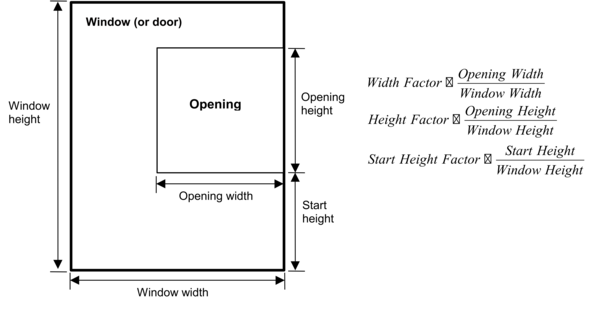
\includegraphics[width=0.9\textwidth, height=0.9\textheight, keepaspectratio=true]{media/image236.png}
\caption{Window (or door) showing geometrical factors associated with an opening through which air flows. \protect \label{fig:window-or-door-showing-geometrical-factors}}
\end{figure}

\paragraph{Field: Opening Factor \textless{}n\textgreater{}}\label{field-opening-factor-n}

When Number of Sets of Opening Factor Data = n, the value of Opening Factor n must be set to 1.0.

\paragraph{Field: Discharge Coefficient for Opening Factor \textless{}n\textgreater{}}\label{field-discharge-coefficient-for-opening-factor-n}

The discharge coefficient of the window or door for Opening Factor n. The range is greater than 0.0 to less than or equal to 1.0. The default value is 1.0.

\paragraph{Field: Width Factor for Opening Factor \textless{}n\textgreater{}}\label{field-width-factor-for-opening-factor-n}

The Width Factor of the rectangular window or door for Opening Factor n. The Width Factor is the opening width divided by the window or door width (see Figure~\ref{fig:window-or-door-showing-geometrical-factors}). The range is 0.0 to 1.0. The default value is 1.0.

\paragraph{Field: Height Factor for Opening Factor \textless{}n\textgreater{}}\label{field-height-factor-for-opening-factor-n}

The Height Factor of the rectangular window or door for Opening Factor n. The Height Factor is the opening height divided by the window or door height (see Figure~\ref{fig:window-or-door-showing-geometrical-factors}). The range is 0.0 to 1.0. The default value is 1.0.

\paragraph{Field: Start Height Factor for Opening Factor \textless{}n\textgreater{}}\label{field-start-height-factor-for-opening-factor-n}

The Start Height Factor of the window or door for Opening Factor n. The Start Height Factor is the Start Height divided by the window or door height (see Figure~\ref{fig:window-or-door-showing-geometrical-factors}). The range is 0.0 to 1.0. The default is 0.

When the opening factor value (as described under the field Window/Door Opening Factor in the \hyperref[airflownetworkmultizonesurface]{AirflowNetwork:MultiZone:Surface} object) is between two Opening Factor field values, the values of Discharge Coefficient, Width Factor, Height Factor, and Start Height Factor are linearly interpolated.

An IDF example is shown below:

\begin{lstlisting}
AirflowNetwork:MultiZone:Component:DetailedOpening,
      WiOpen1,                 !- Detailed Opening Name
      0.001,                   !- Air Mass Flow Coefficient When Opening is Closed {kg/s-m}
      0.667,                   !- Air Mass Flow Exponent When Opening is Closed {dimensionless}
      NonPivoted,             !- Type of Large Vertical Opening (LVO)
      0.0,                     !- Extra crack length for LVO type 1 with multiple openable parts,
                               !- or Height of pivoting axis for LVO type 2 {m}
      2,                       !- Number of Sets of Opening Factor Data
      0.0,                     !- Opening factor 1 {dimensionless}
      0.5,                     !- Discharge coefficient for opening factor 1 {dimensionless}
      0.0,                     !- Width factor for opening factor 1 {dimensionless}
      1.0,                     !- Height factor for opening factor 1 {dimensionless}
      0.0,                     !- Start height factor for opening factor 1 {dimensionless}
      1.0,  0.6,  1.0,  1.0,  0.0;  !-  Set of values for opening factor 2
\end{lstlisting}

\subsection{AirflowNetwork:MultiZone:Component:HorizontalOpening}\label{airflownetworkmultizonecomponenthorizontalopening}

This object specifies the properties of air flow through windows, doors and glass doors (heat transfer subsurfaces defined as a subset of \hyperref[fenestrationsurfacedetailed]{FenestrationSurface:Detailed} objects) when they are closed or open. This AirflowNetwork model assumes that these openings are horizontal or close to horizontal and are interzone surfaces. The second and third input fields are similar to those for \hyperref[airflownetworkmultizonesurfacecrack]{AirflowNetwork:MultiZone:Surface:Crack}, when the window or door is closed, but additional information is required to describe the air flow characteristics when the window or door is open. This additional information is specified in the last two input fields. The airflow across the opening consists of two types of flows: forced and buoyancy. The forced flow is caused by the pressure difference between two zones, while the buoyancy flow only occurs when the air density in the upper zone is greater than the air density in the lower zone. This opening also allows for the possibility of two-way flow when forced and buoyancy flows co-exist. This object's openness can also be modulated based on the same opening factor control as an \hyperref[airflownetworkmultizonecomponentdetailedopening]{AirflowNetwork:MultiZone:Component:DetailedOpening} object. However, the opening factor is only applied to the subsurface width. The opening width is equal to opening factor multiplied by the subsurface width.

A subsurface multiplier may be used to represent multiple subsurfaces and calculates total air flow when the subsurface (window, glassdoor, or door) is either closed or open. The total airflow across the surface is equal to the airflow based on the surface geometry multiplied by the subsurface multiplier.

\subsubsection{Inputs}\label{inputs-5-003}

\paragraph{Field: Name}\label{field-name-5-003}

This is a name for this AirflowNetwork:MultiZone:Component:HorizontalOpening object. It is referenced by an \hyperref[airflownetworkmultizonesurface]{AirflowNetwork:MultiZone:Surface} object.

\paragraph{Field: Air Mass Flow Coefficient When Opening is Closed}\label{field-air-mass-flow-coefficient-when-opening-is-closed-1}

The value of the air mass flow coefficient, \({C_{Q,\;unit\;length}}\) , in the horizontal opening air flow equation. It has units of kg/s-m at 1Pa. The temperature correction factor is not applied to the mass flow calculation. This is a required input field and the entered value must be greater than zero.

\paragraph{Field: Air Mass Flow Exponent When Opening is Closed}\label{field-air-mass-flow-exponent-when-opening-is-closed-1}

The value of the exponent, \emph{n}, in the crack air flow equation. The valid range is 0.5 to 1.0, with the default value being 0.65.

\paragraph{Field: Sloping Plane Angle}\label{field-sloping-plane-angle}

This numeric field is used to represent the angle between the horizontal plane and a sloped plane under the horizontal opening. Sloping plane angle = 90 is equivalent to fully open. The valid range is \textgreater{}0 to 90, with the default value being 90.

\paragraph{Field: Discharge Coefficient}\label{field-discharge-coefficient-1}

This numeric field is used to input the discharge coefficient. This is a required field and the entered value must be greater than zero.

An IDF example is shown below:

\begin{lstlisting}
AirflowNetwork:MultiZone:Component:HorizontalOpening,
      HrOpen,                  !- Name
      0.001,                   !- Air Mass Flow Coefficient When Opening is Closed {kg/s-m}
      0.667,                   !- Air Mass Flow Exponent When Opening is Closed {dimensionless}
      90.0,                    !- Sloping Plane Angle
      0.2;                     !- Discharge Coefficient
\end{lstlisting}

\subsection{AirflowNetwork:MultiZone:Component:SimpleOpening}\label{airflownetworkmultizonecomponentsimpleopening}

This object specifies the properties of air flow through windows, doors and glass doors (heat transfer subsurfaces) when they are closed or open. The AirflowNetwork model assumes that open windows or doors are vertical or close to vertical. The second and third fields are similar to those for \hyperref[airflownetworkmultizonesurfacecrack]{AirflowNetwork:MultiZone:Surface:Crack}, when the window or door is closed, but additional information is required to describe the air flow characteristics when the window or door is open. This additional information is specified in the last two fields. Compared to the object \hyperref[airflownetworkmultizonecomponentdetailedopening]{AirflowNetwork:MultiZone:Component:DetailedOpening}, which requires more inputs at different opening factors, this object needs comparatively less inputs. For this reason it is called a simple opening. This opening also allows for the possibility of two-way flow due to temperature and resulting density differences. Therefore, it is possible to have a positive pressure difference at the top of the opening, and a negative pressure difference at the bottom (or vice versa) when the neutral height is between the bottom and top heights of the associated surface. This object's openness can also be modulated based on the same opening factor control as an \hyperref[airflownetworkmultizonecomponentdetailedopening]{AirflowNetwork:MultiZone:Component:DetailedOpening} object. However, the opening factor is only applied to the subsurface width. The opening width is equal to opening factor multiplied by the subsurface width.

A subsurface multiplier may be used to represent multiple subsurfaces and calculates total air flow when the subsurface (window, glassdoor, or door) is either closed or open. The total airflow across the surface is equal to the airflow based on the surface geometry multiplied by the subsurface multiplier.

\subsubsection{Inputs}\label{inputs-6-002}

\paragraph{Field: Name}\label{field-name-6-002}

This is a name for this AirflowNetwork:MultiZone:Component:SimpleOpening object. It is referenced by an \hyperref[airflownetworkmultizonesurface]{AirflowNetwork:MultiZone:Surface} object.

\paragraph{Field: Air Mass Flow Coefficient When Opening is Closed}\label{field-air-mass-flow-coefficient-when-opening-is-closed-2}

The value of the air mass flow coefficient, \({C_{Q,\;unit\;length}}\) , in the simple opening air flow equation. It has units of kg/s-m at 1Pa. The temperature correction factor is not applied for mass flow calculation.

\paragraph{Field: Air Mass Flow Exponent When Opening is Closed}\label{field-air-mass-flow-exponent-when-opening-is-closed-2}

The value of the exponent, n\emph{, in the crack air flow equation. The valid range is 0.5 to 1.0, with the default value being 0.65. Mass Flow Rate = Air Mass Flow Coefficient} (deltaP)\^{}Air Mass Flow Exponent.

\paragraph{Field: Minimum Density Difference for Two-Way Flow}\label{field-minimum-density-difference-for-two-way-flow}

This numeric field is used to input the minimum density difference above which two-way or one way flow may occur due to stack effect with the window being open. Two-way flow occurs only when the neutral plane is within the opening. Density differences less than this value result in one-way flow only with the window being closed. The minimum value for this field is greater than zero.

\paragraph{Field: Discharge Coefficient}\label{field-discharge-coefficient-2}

This numeric field is used to input the discharge coefficient. This value must be greater than zero.

An IDF example is shown below:

\begin{lstlisting}
 AirflowNetwork:MultiZone:Component:SimpleOpening,
      WiOpen2,                 !- Simple Opening Name
      0.001,                   !- Air Mass Flow Coefficient When Opening Is Closed {kg/s-m}
      0.650,                   !- Air Mass Flow Exponent When Opening Is Closed {dimensionless}
      0.0001,                  !- Minimum density difference for two-way flow (kg/m3)
      1.0;                     !- Discharge coefficient (dimensionless)
\end{lstlisting}

\subsection{AirflowNetwork:MultiZone:Component:ZoneExhaustFan}\label{airflownetworkmultizonecomponentzoneexhaustfan}

This object specifies the properties of air flow through an exterior heat transfer surface with a zone exhaust fan. The zone exhaust fan turns on or off based on the availability schedule defined in the corresponding \hyperref[fanzoneexhaust]{Fan:ZoneExhaust} object. When the exhaust fan mass flow rate is greater than zero, the airflow network model treats this object as a constant volume fan. When the fan is off based on the availability schedule, the model treats this object as a crack.

When the fan is on, the air mass flow rate modeled for the airflow network is based on the value defined in the MaximumFlow Rate field of the \hyperref[fanzoneexhaust]{Fan:ZoneExhaust} object. The airflow direction is from the corresponding zone to outdoors.

When the fan is off, the following power law form is used that gives air flow through the crack as a function of the pressure difference across the crack:

\begin{equation}
Q = \left( Crack\;Factor \right) * C_T * C_Q \left( \Delta P \right)^{n}
\end{equation}

Where

\emph{Q}~~~ = air mass flow (kg/s)

\emph{C\(_{Q}\)}~ = air mass flow coefficient (kg/s-Pa\(^{n}\) @ 1 Pa)

\emph{C\(_{T}\)}~ = reference condition temperature correction factor (dimensionless)

\(\Delta P\) = pressure difference across crack (Pa)

\emph{n}~~~ = air flow exponent (dimensionless)

\begin{equation}
{C_T} = {\left[ {\frac{{{\rho_o}}}{\rho }} \right]^{n - 1}}{\left[ {\frac{{{\nu_o}}}{\nu }} \right]^{2n - 1}}
\end{equation}

where

\(\rho\) = Air density at the specific air temperature and humidity ratio conditions {[}kg/m\(^{3}\){]}

\(\nu\) = Air kinetic viscosity at the specific air temperature condition {[}m\(^{2}\)/s{]}

\(\rho_o\) = Air density at the reference air conditions provided by the object Air\-flow\-Net\-work:\-Multi\-Zone:\-Reference\-Crack\-Con\-ditions specified in the field Reference Crack Conditions {[}kg/m\(^{3}\){]}

\(\nu_o\) = Air kinetic viscosity at the reference air temperature provided by the object Air\-flow\-Net\-work:\-Multi\-Zone:\-Reference\-Crack\-Con\-ditions specified in the field Reference Crack Conditions {[}m\(^{2}\)/s{]}

Note: The correction factor shown above is used when the exhaust fan is off. The airflow direction is based on the pressure difference between the zone and outdoors.

\subsubsection{Inputs}\label{inputs-7-002}

\paragraph{Field: Name}\label{field-name-7-001}

This is the name for this instance of the Air\-flow\-Net\-work:\-Multi\-Zone:\-Com\-ponent:\-Zone\-Exhaust\-Fan object. This name must be the same name defined in the Fan:\-Zone\-Exhaust object. It is referenced by an Air\-flow\-Net\-work:\-Multi\-zone:\-Sur\-face object.

\paragraph{Field: Air Mass Flow Coefficient When the Zone Exhaust Fan is Off at Reference Conditions}\label{field-air-mass-flow-coefficient-when-the-zone-exhaust-fan-is-off-at-reference-conditions}

The value of the air mass flow coefficient,\({C_Q}\) , in the crack air flow equation. It has units of kg/s at 1Pa. This value must be greater than zero. The value is used when the fan is off.

\paragraph{Field: Air Mass Flow Exponent When the Zone Exhaust Fan is Off}\label{field-air-mass-flow-exponent-when-the-zone-exhaust-fan-is-off}

The value of the exponent, \emph{n}, in the crack air flow equation. The valid range is 0.5 to 1.0, with the default value being 0.65. The value is used when the fan is off.

\paragraph{Field: Reference Crack Conditions}\label{field-reference-crack-conditions-1}

The name of the \hyperref[airflownetworkmultizonereferencecrackconditions]{AirflowNetwork:MultiZone:ReferenceCrackConditions} object which specifies the conditions under which the air mass flow coefficient was measured. If the user omits this field and only one \hyperref[airflownetworkmultizonereferencecrackconditions]{AirflowNetwork:MultiZone:ReferenceCrackConditions} object is defined in the input data file, then those reference crack conditions will be used. If the user omits this field and either zero or more than one \hyperref[airflownetworkmultizonereferencecrackconditions]{AirflowNetwork:MultiZone:ReferenceCrackConditions} objects are defined in the input data file, then the default conditions for the AirflowNetwork:MultiZone: Reference Crack Conditions object will be used.

An IDF example is shown below:

\begin{lstlisting}

AirflowNetwork:MultiZone:Component:ZoneExhaustFan,
      Zone3 Exhaust Fan,       !- Name
      0.01,     !- Air Mass Flow Coefficient When the Zone Exhaust Fan is Off at Reference Conditions {kg/s}
      0.667;    !- Air Mass Flow Exponent When the Zone Exhaust Fan is Off{dimensionless}
      ReferenceCrackConditions; !- Reference Crack Conditions
\end{lstlisting}

\subsection{AirflowNetwork:MultiZone:ExternalNode}\label{airflownetworkmultizoneexternalnode}

External nodes in the AirflowNetwork model define environmental conditions
outside of the building. These conditions include wind pressure coefficients
that vary from fa\c{c}ade to fa\c{c}ade and can be highly dependent on the
building geometry.

AirflowNetwork:MultiZone:ExternalNode objects do \textbf{not} have to be
entered if Wind Pressure Coefficient Type = SurfaceAverageCalculation in the
\hyperref[airflownetworksimulationcontrol]{AirflowNetwork:\hyperref[simulationcontrol]{SimulationControl}} object.

\subsubsection{Inputs}\label{inputs-8-001}

\paragraph{Field: Name}\label{field-name-8-001}

The external node name is associated with a particular building fa\c{c}ade.
This name is referenced by the External Node Name field of an \hyperref[airflownetworkmultizonesurface]{AirflowNetwork:MultiZone:Surface} object.

\paragraph{Field: External Node Height}\label{field-external-node-height}

Designates the reference height, in meters, used to calculate relative pressure. The default value is 0 meters.

\paragraph{Field: Wind Pressure Coefficient Curve Name}\label{field-wind-pressure-coefficient-values-object-name}

The name of a specific \hyperref[airflownetworkmultizonewindpressurecoefficientvalues]{AirflowNetwork:MultiZone:WindPressureCoefficientValues}
object, curve, or table (which gives wind pressure coefficients for the
fa\c{c}ade as a function of angle of wind incident on the fa\c{c}ade). Curves
or tables should have the domain of 0 to 180 degrees or 0 to 360 degrees,
depending upon the symmetry field (see below).

\paragraph{Field: Symmetric Wind Pressure Coefficient Curve}\label{field-symmetric-wind-pressure-coefficient}
Specifies the symmetry of the above named curve. The default is No, meaning
that the curve will be evaluated from 0 to 360 degrees. Specify Yes for a
curve that is symmetric about zero and is evaluated only up to 180 degrees.
For this type of curve, an angle of 270 degrees is passed to the curve as
90 degrees.

\paragraph{Field: Wind Angle Type}\label{field-wind-angle-type}
Specifies which wind angle should be used to calculate the wind pressure
coefficient. The default is Absolute, meaning that the absolute wind direction
angle will be used. Specifying Relative means that the angle will be relative
to the surface normal. For a surface facing due east, the angle 0 corresponds
to wind blowing perpendicular to and at the surface with absolute direction
90 degrees, while 90 degrees corresponds to wind blowing parallel to the
surface from the right (facing outward) with an absolute direction of 180 degrees.

IDF examples are provided below:

\begin{lstlisting}
AirflowNetwork:MultiZone:ExternalNode,
      NFacade,                 !- Name
      1.524,                   !- External Node Height {m}
      NFacade_WPCValue;        !- Wind Pressure Coefficient Curve Name

  AirflowNetwork:MultiZone:ExternalNode,
      EFacade,                 !- Name
      1.524,                   !- External Node Height {m}
      EFacade_WPCValue;        !- Wind Pressure Coefficient Curve Name

  AirflowNetwork:MultiZone:ExternalNode,
      SFacade,                 !- Name
      1.524,                   !- External Node Height {m}
      SFacade_WPCValue;        !- Wind Pressure Coefficient Curve Name

  AirflowNetwork:MultiZone:ExternalNode,
      WFacade,                 !- Name
      1.524,                   !- External Node Height {m}
      WFacade_WPCValue;        !- Wind Pressure Coefficient Curve Name

  AirflowNetwork:MultiZone:ExternalNode,
      Horizontal,              !- Name
      3.028,                   !- External Node Height {m}
      Horizontal_WPCValue;     !- Wind Pressure Coefficient Curve Name
\end{lstlisting}

\subsection{AirflowNetwork:MultiZone:WindPressureCoefficientArray}\label{airflownetworkmultizonewindpressurecoefficientarray}

The reference height and wind directions are first specified under the AirflowNetwork:MultiZone:WindPressureCoefficientArray object. The user may specify up to 36 different wind directions in ascending order. These are then referenced by \hyperref[airflownetworkmultizonewindpressurecoefficientvalues]{AirflowNetwork:MultiZone:WindPressureCoefficientValues} objects defined for each \hyperref[airflownetworkmultizoneexternalnode]{AirflowNetwork:MultiZone:ExternalNode}.

The AirflowNetwork:MultiZone:WindPressureCoefficientArray object is unique and needs to be entered only if Wind Pressure Coefficient Type = INPUT in the \hyperref[airflownetworksimulationcontrol]{AirflowNetwork:\hyperref[simulationcontrol]{SimulationControl}} object. If Wind Pressure Coefficient Type = SurfaceAverageCalculation, this object is not required.

\subsubsection{Inputs}\label{inputs-9-001}

\paragraph{Field: Name}\label{field-name-9-001}

The name of this AirflowNetwork:MultiZone:WindPressureCoefficientArray object. This name is referenced by each \hyperref[airflownetworkmultizonewindpressurecoefficientvalues]{AirflowNetwork:MultiZone:WindPressureCoefficientValues} object which, for each \hyperref[airflownetworkmultizoneexternalnode]{AirflowNetwork:MultiZone:ExternalNode}, gives the wind pressure coefficients at each of the wind directions listed in the AirflowNetwork:MultiZone:WindPressureCoefficientArray. This name is also referenced by the \hyperref[airflownetworksimulationcontrol]{AirflowNetwork:\hyperref[simulationcontrol]{SimulationControl}} object, indicating that this AirflowNetwork:MultiZone:WindPressureCoefficientArray and the pressure coefficients in the associated \hyperref[airflownetworkmultizonewindpressurecoefficientvalues]{AirflowNetwork:MultiZone:WindPressureCoefficientValues} objects will be used in the air flow simulation.

\paragraph{Field: Wind Direction 1-Wind Direction N}\label{field-wind-direction-1-wind-direction-n}

Each field references the wind direction corresponding to the first through the Nth WPC value in each of the \hyperref[airflownetworkmultizonewindpressurecoefficientvalues]{AirflowNetwork:MultiZone:WindPressureCoefficientValues} objects. \emph{N} can be as high as 36.

An IDF example is provided below:

\begin{lstlisting}
AirflowNetwork:MultiZone:WindPressureCoefficientArray,
      Every 30 Degrees,        !- WPC Array Name
      0,                       !- Wind Direction #1 {deg}
      30,                      !- Wind Direction #2 {deg}
      60,                      !- Wind Direction #3 {deg}
      90,                      !- Wind Direction #4 {deg}
      120,                     !- Wind Direction #5 {deg}
      150,                     !- Wind Direction #6 {deg}
      180,                     !- Wind Direction #7 {deg}
      210,                     !- Wind Direction #8 {deg}
      240,                     !- Wind Direction #9 {deg}
      270,                     !- Wind Direction #10 {deg}
      300,                     !- Wind Direction #11 {deg}
      330;                     !- Wind Direction #12 {deg}
\end{lstlisting}

\subsection{AirflowNetwork:MultiZone:WindPressureCoefficientValues}\label{airflownetworkmultizonewindpressurecoefficientvalues}

This object specifies up to 36 wind pressure coefficients (WPCs) for an \hyperref[airflownetworkmultizoneexternalnode]{AirflowNetwork:MultiZone:ExternalNode}. These coefficients are defined for each of the wind directions defined in the unique \hyperref[airflownetworkmultizonewindpressurecoefficientarray]{AirflowNetwork:MultiZone:WindPressureCoefficientArray} object. In the air flow calculation, interpolation of the specified WPC values is done for time-step values of wind direction.

AirflowNetwork:MultiZone:WindPressureCoefficientValues objects need to be entered only if the Wind Pressure Coefficient Type = INPUT in the \hyperref[airflownetworksimulationcontrol]{AirflowNetwork:\hyperref[simulationcontrol]{SimulationControl}} object. If Wind Pressure Coefficient Type = SurfaceAverageCalculation, this object is not required and is not used.

\subsubsection{Inputs}\label{inputs-10-001}

\paragraph{Field: Name}\label{field-name-10-001}

The name of this WindPressureCoefficientValues object. This name can be referenced by multiple \hyperref[airflownetworkmultizoneexternalnode]{AirflowNetwork:MultiZone:ExternalNode} objects.

\paragraph{Field: WindPressureCoefficientArray Name}\label{field-windpressurecoefficientarray-name}

Name of the associated \hyperref[airflownetworkmultizonewindpressurecoefficientarray]{AirflowNetwork:MultiZone:WindPressureCoefficientArray}, which lists the wind direction corresponding to each wind pressure coefficient value in this AirflowNetwork:MultiZone:WindPressureCoefficientValues object.

\paragraph{Field: Wind Pressure Coefficient Value 1 to Wind Pressure Coefficient Value N}\label{field-wind-pressure-coefficient-value-1-to-wind-pressure-coefficient-value-n}

The WPC (wind pressure coefficient) value for the building fa\c{c}ade indicated by the External Node Name field above. This WPC value corresponds to the first wind direction in the \hyperref[airflownetworkmultizonewindpressurecoefficientarray]{AirflowNetwork:MultiZone:WindPressureCoefficientArray}. Note that WPC values can be positive, negative or zero.

\paragraph{Obtaining WPC values}\label{obtaining-wpc-values}

WPC values can be obtained from wind tunnel measurements, CFD calculations, or from published values for different building shapes.

For \textbf{rectangular buildings} EnergyPlus will automatically calculate surface-averaged Cp values for the walls and roof of the building if you specify Wind Pressure Coefficient Type = SurfaceAverageCalculation in the \hyperref[airflownetworksimulationcontrol]{AirflowNetwork:\hyperref[simulationcontrol]{SimulationControl}} object. In this case you do not have to enter any AirflowNetwork:MultiZone:WindPressureCoefficientValues objects.

Wind pressure coefficients are reported in the eplusout.eio either from inputs using ``INPUT'' as the choice for the Wind Pressure Coefficient Type field defined in the \hyperref[airflownetworksimulationcontrol]{AirflowNetwork:\hyperref[simulationcontrol]{SimulationControl}} object, or from internal calculation using SurfaceAverageCalculation as the choice for the Wind Pressure Coefficient Type field defined in the same object. Below is an output example from the eplusout.eio file:

\begin{lstlisting}
AirflowNetwork Model:Wind Direction, 0.0,30.0,60.0,90.0,120.0,150.0,180.0,210.0,240.0,270.0,300.0,330.0
! <AirflowNetwork Model:Wind Pressure Coefficients, WPC Name, Wind Pressure Coefficients #1 to n (dimensionless)>
AirflowNetwork Model:Wind Pressure Coefficients, NFACADE, 0.60,0.48,4.00E-002,-0.56,-0.56,-0.42,-0.37,-0.42,-0.56,-0.56,4.00E-002,0.48
AirflowNetwork Model:Wind Pressure Coefficients, EFACADE, -0.56,4.00E-002,0.48,0.60,0.48,4.00E-002,-0.56,-0.56,-0.42,-0.37,-0.42,-0.56
AirflowNetwork Model:Wind Pressure Coefficients, SFACADE, -0.37,-0.42,-0.56,-0.56,4.00E-002,0.48,0.60,0.48,4.00E-002,-0.56,-0.56,-0.42
AirflowNetwork Model:Wind Pressure Coefficients, WFACADE, -0.56,-0.56,-0.42,-0.37,-0.42,-0.56,-0.56,4.00E-002,0.48,0.60,0.48,4.00E-002
\end{lstlisting}

An IDF example is provided below:

\begin{lstlisting}
AirflowNetwork:MultiZone:WindPressureCoefficientValues,
      NFacade_WPCValue,        !- Name
      Every 30 Degrees,        !- AirflowNetwork:MultiZone:WindPressureCoefficientArray Name
      0.60,                    !- Wind Pressure Coefficient Value 1 {dimensionless}
      0.48,                    !- Wind Pressure Coefficient Value 2 {dimensionless}
      0.04,                    !- Wind Pressure Coefficient Value 3 {dimensionless}
      -0.56,                   !- Wind Pressure Coefficient Value 4 {dimensionless}
      -0.56,                   !- Wind Pressure Coefficient Value 5 {dimensionless}
      -0.42,                   !- Wind Pressure Coefficient Value 6 {dimensionless}
      -0.37,                   !- Wind Pressure Coefficient Value 7 {dimensionless}
      -0.42,                   !- Wind Pressure Coefficient Value 8 {dimensionless}
      -0.56,                   !- Wind Pressure Coefficient Value 9 {dimensionless}
      -0.56,                   !- Wind Pressure Coefficient Value 10 {dimensionless}
      0.04,                    !- Wind Pressure Coefficient Value 11 {dimensionless}
      0.48;                    !- Wind Pressure Coefficient Value 12 {dimensionless}
\end{lstlisting}

\subsection{AirflowNetwork:OccupantVentilationControl}\label{airflownetworkoccupantventilationcontrol}

The AirflowNetwork:OccupantVentilationControl object provides control options with minimum opening and closing time checks and opening and closing probability values. In general, the probability values could be a constant or a specific function. Due to lack of real data, two schedules are selected to represent probability values. If real data are available, this object may be modified to adopt new data.

\subsubsection{Inputs}\label{inputs-11-001}

\paragraph{Field: Name}\label{field-name-11-001}

This is the name of the object.

\paragraph{Field: Minimum Opening Time}\label{field-minimum-opening-time}

The field represents the minimum time that windows will remain open. If a window has been open for a time less than this value, the window will remain open.

\paragraph{Field: Minimum Closing Time}\label{field-minimum-closing-time}

The field represents the minimum time that windows will remain closed. If a window has been closed for a time less than this value, the window will remain closed.

\paragraph{Field: Thermal Comfort Low Temperature Curve Name}\label{field-thermal-comfort-low-temperature-curve-name}

This alpha field defines the name of a curve to be used for thermal comfort temperature calculation at low outdoor dry-bulb temperature. This curve is a linear or quadratic equation using outdoor dry-bulb temperatures as an independent variable. This performance curve can be used to describe the thermal comfort temperature at low outdoor dry-bulb temperature. It allows maximum two curves to describe the thermal comfort temperature in two different outdoor dry-bulb temperature regions. If a single curve is used, blanks are entered in the following two fields.

\paragraph{Field: Thermal Comfort Temperature Boundary Point}\label{field-thermal-comfort-temperature-boundary-point}

When there are two piecewise curves to represent thermal comfort temperature calculation, this field represents a boundary point of outdoor dry-bulb temperature. The low temperature curve and the high temperature curve should have the same values at the boundary point. If a single curve is used, this field may be left blank.

\paragraph{Field: Thermal Comfort High Temperature Curve Name}\label{field-thermal-comfort-high-temperature-curve-name}

This alpha field defines the name of a curve to be used for thermal comfort temperature calculation at high outdoor dry-bulb temperature. This curve is a linear or quadratic equation using outdoor dry-bulb temperatures as an independent variable. This performance curve can be used to describe the thermal comfort temperature at high outdoor dry-bulb temperature. It allows maximum two curves to describe the thermal comfort temperature in two different outdoor dry-bulb temperature regions. If a single curve is used, blanks are entered in this field.

\paragraph{Field: Maximum Threshold for Persons Dissatisfied PPD}\label{field-maximum-threshold-for-persons-dissatisfied-ppd}

This field is used to calculate the comfort band as a function of predicted percentage of dissatisfied (PPD). The default value is 10\%. The equation is based on curve fit and is valid between 0\% and 35\%.

\begin{equation}
\Theta = -0.0028 (100-PPD)^2 + 0.3419 (100-PPD) - 6.6275
\end{equation}

where

\begin{itemize}
\tightlist
\item
  \(\Theta\) is the comfort band (degC)
\item
  PPD is predicted percentage person of dissatisfied (\%)
\end{itemize}

\paragraph{Field: Occupancy Check}\label{field-occupancy-check}

Input is Yes or No. The default is No. If Yes, an occupancy check is performed used in the opening probability check. If No, the occupancy check is bypassed.

\paragraph{Field: Opening Probability Schedule Name}\label{field-opening-probability-schedule-name}

The name of a schedule of opening probability that controls the opening of windows and doors in the thermal zone to provide natural ventilation. If the probability value is greater a random number, windows are allowed to open. Otherwise, the output will be false. This control will occur when minimum time checks for both opening and closing are satisfied.

\paragraph{Field: Closing Probability Schedule Name}\label{field-closing-probability-schedule-name}

The name of a schedule of closing probability that controls the closing of windows and doors in the thermal zone to reduce natural ventilation. If the probability value is greater a random number, windows are allowed to be closed. Otherwise, the output will be false. This control will occur when minimum time checks for both opening and closing are satisfied.

An IDF example is provided below:

\begin{lstlisting}
AirlowNetwork:OccupantVentilationControl,
  VentilationControl,      !- Name
  5.0,                     !- Minimum Opening Time
  5.0,                     !- Minimum Opening Time
  ComfortLowTempCurve,     !- Thermal Comfort Low Temperature Curve Name
  10.0,                    !- Thermal Comfort Temperature Boundary Point
  ComfortHighTempCurve,    !- Thermal Comfort High Temperature Curve Name
  10.0,                    !- Maximum Threshold for Persons Dissatisfied PPD
  Yes,                     !- Occupancy Check
  OpeningProbabilitySch,   !- Opening Probability Schedule Name
  ClosingProbabilitySch;   !- Closing Probability Schedule Name
\end{lstlisting}

\subsection{AirflowNetwork:ZoneControl:PressureController}\label{airflowNetworkzonecontrolpressureoontroller}

The AirflowNetwork:ZoneControl:PressureController object is used to control a zone to a specified indoor level of pressure using the AirflowNetwork model. The specified pressure setpoint is used to calculate the required zone exhaust fan flow rate in a controlled zone or relief air flow rate in an AirLoop.

The object has a similar function as \hyperref[zonecontrolthermostat]{ZoneControl:Thermostat}. When an AirLoop serves multiple zones, the controlled zone will reach the specified setpoint, while other zones will not be controlled precisely.

\subsubsection{Inputs}\label{inputs-AFN-pressure-control}

\paragraph{Field: Name}\label{field-name-AFN-pressure-control}

Unique identifying name for the AirflowNetwork:ZoneControl:PressureController.

\paragraph{ Field: Control Zone Name}\label{field-control-zone-name}

Name of the zone that is being controlled.

\paragraph{ Field: Control Object Type}\label{field-control-object-type}

This field specifies the control type to be used for pressure control. Available control types are:
\hyperref[airflownetworkmultizonecomponentzoneexhaustfan]{AirflowNetwork:MultiZone:Component:ZoneExhaustFan} and \hyperref[airflowNetworkdistributioncomponentreliefairflow]{AirflowNetwork:Distribution:Component:ReliefAirFlow}.

\paragraph{ Field: Control Object Name}\label{field-control-name}

The corresponding control object name.

\paragraph{ Field: Pressure Control Availability Schedule Name}\label{field-pressure-control-availability-schedule-name}

This field contains the name of a schedule that determines whether or not the AirflowNetwork:ZoneControl:PressureController is available. When the schedule value is zero, the AirflowNetwork:ZoneControl:PressureController is bypassed (not available to operate). When the schedule value is greater than zero, the AirflowNetwork:ZoneControl:PressureController is available to perform pressure control. When AirflowNetwork:Distribution:Component:ZoneExhaustFan in entered in the Control Object Type field, the model will calculate the required zone exhaust fan airflow rate to reach the pressure setpoint. When an \hyperref[airflowNetworkdistributioncomponentreliefairflow]{AirflowNetwork:Distribution:Component:ReliefAirFlow} is entered in the Control Object Type field, the model will calculate the central relief flow rate in an outdoor air mixer. If this field is left blank, the schedule has a value of 1 for all time periods. Schedule values must be between 0 and 1.

\paragraph{ Field: Pressure Setpoint Schedule Name}\label{field-pressure-setpoint-schedule-name}

This field contains the name of a schedule that contains the zone air pressure setpoint as a function of time. The units for pressure setpoint are Pascal. The setpoint values in the schedule must be between -50 and 100 Pascal.

An IDF example is provided below:

\begin{lstlisting}
AirflowNetwork:ZoneControl:PressureController,
  Pressure Controller1,           !- Name
  EAST ZONE,                      !- Controlled Zone Name
  AirflowNetwork:MultiZone:Component:ZoneExhaustFan, !- Control Object type
  East Zone Exhaust Fan,          !- Control Object Name
  PressureAvailSchedule,          !- Pressure Control Availability Schedule Name
  PressureSetpointSchedule;       !- Pressure Setpoint Schedule Name
\end{lstlisting}

\subsection{AirflowNetwork with RoomAir Models}\label{airflownetwork-roomair-models}

The next two objects of \hyperref[airflownetworkintrazonenode]{AirflowNetwork:IntraZone:Node} and \hyperref[airflownetworkintrazonelinkage]{AirflowNetwork:IntraZone:Linkage} are used with \hyperref[roomairnodeairflownetwork]{RoomAir:Node:AirflowNetwork} objects together to simulate multiple internal airflows via multiple intrazone nodes and linkages in a thermal zone. The mixed-air assumption for zone air conditions is not always appropriate. EnergyPlus includes several RoomAir models that can model the implications for different flow patterns on variations in temperature within the zone. However none of them are generalized enough for different types of air flow situations and none are coupled tightly with AirflowNetwork. A general RoomAir model based on pressure network solver will allow modeling a variety of spaces types not currently covered by existing models such as tall spaces.

Recent advancements have been made to AirflowNetwork to model large horizontal openings. This new development makes AirflowNetwork useful for not only modeling air movement between zones (and outdoors), but also within individual thermal zones.

The possible combination will allow the EnergyPlus to simulate a thermal zone using a network approach by assuming internal nodes connected by user-defined patterns of temperatures and airflows. It should be pointed out that the new model works when the MultiZoneWithoutDistribution is selected in the field of AirflowNetwork Control of the \hyperref[airflownetworksimulationcontrol]{AirflowNetwork:\hyperref[simulationcontrol]{SimulationControl}} object. The model cannot work with other choices.

\subsection{AirflowNetwork:IntraZone:Node}\label{airflownetworkintrazonenode}

This object allows users to input multiple nodes in a zone. A single object represent a node. If there is only one node per zone, then use the \hyperref[airflownetworkmultizonezone]{AirflowNetwork:MultiZone:Zone} input object. The zone node is not defined in this object.

\subsubsection{Field: Name}\label{field-name-12-000}

The name identifies the node for later reference and in the output listing. Each node should have a unique name. This name can be referenced as AirflowNetworkNodeNames.

\subsubsection{Field: RoomAir:Node:AirflowNetwork Name}\label{field-roomairnodeairflownetwork-name}

The name of a \hyperref[roomairnodeairflownetwork]{RoomAir:Node:AirflowNetwork} object, which is also defined in a \hyperref[roomairsettingsairflownetwork]{RoomAirSettings:AirflowNetwork} object (zone based).

\subsubsection{Field: Zone Name}\label{field-zone-name-1-000}

The name of a zone object, which is also defined in a \hyperref[airflownetworkmultizonezone]{AirflowNetwork:MultiZone:Zone} object (zone based).

\subsubsection{Field: Node Height}\label{field-node-height}

This field requires input of node height in meters.

An IDF example is provided below:

VentilationControl, !- Name

\begin{lstlisting}
AirflowNetwork:IntraZone:Node,
  LeftUpper,               !- Name
  LeftUpper,               !- RoomAir:Node:AirflowNetwork Name
  NORTH_ZONE,              !- Zone Name
  4.572;                   !- Node Height {m}
\end{lstlisting}

\subsection{AirflowNetwork:IntraZone:Linkage}\label{airflownetworkintrazonelinkage}

The input object specifies a connection between two \hyperref[airflownetworkintrazonenode]{AirflowNetwork:IntraZone:Node} objects and an AiflowNetwork component defined elsewhere. The object also allow users to specify a connection between an \hyperref[airflownetworkintrazonenode]{AirflowNetwork:IntraZone:Node} and an adjacent zone defined in an \hyperref[airflownetworkmultizonezone]{AirflowNetwork:MultiZone:Zone} object. This object provides flexibility to define a linkage either in the same zone or in two different zones.

\subsubsection{Field: Name}\label{field-name-13-000}

The name identifies the linkage for later reference and in the output listing. Each linkage should have a unique name.

\subsubsection{Field: Node 1 Name}\label{field-node-1-name}

The input designates a node name where airflow starts. The node name should be defined in an \hyperref[airflownetworkintrazonenode]{AirflowNetwork:IntraZone:Node} object or an \hyperref[airflownetworkmultizonezone]{AirflowNetwork:MultiZone:Zone} object.

\subsubsection{Field: Node 2 Name}\label{field-node-2-name}

The input designates a node name where airflow ends. The node name should be defined in an \hyperref[airflownetworkintrazonenode]{AirflowNetwork:IntraZone:Node} object or an \hyperref[airflownetworkmultizonezone]{AirflowNetwork:MultiZone:Zone} object.

Note: One of Node 1 and Node 2 should be defined as an \hyperref[airflownetworkintrazonenode]{AirflowNetwork:IntraZone:Node} object. In other words, both nodes cannot be defined as \hyperref[airflownetworkmultizonezone]{AirflowNetwork:MultiZone:Zone} object. This type of connection should be defined as an \hyperref[airflownetworkmultizonesurface]{AirflowNetwork:MultiZone:Surface} object.

\subsubsection{Field: Component Name}\label{field-component-name-000}

The input designates an AirflowNetwork component name associated with the two nodes. The component name should be one of the AirflowNetwork:MultiZone:Component object names. The component is used for intrazone node connection only. If the next field is specified, the input of this field could be a blank.

It should be pointed out that an \hyperref[airflownetworkmultizonesurface]{AirflowNetwork:MultiZone:Surface} object allows following five AirflowNetwork:MultiZone:Component objects:

\begin{itemize}
\tightlist
\item
  \hyperref[airflownetworkmultizonecomponentdetailedopening]{AirflowNetwork:MultiZone:Component:DetailedOpening},
\item
  \hyperref[airflownetworkmultizonecomponentsimpleopening]{AirflowNetwork:MultiZone:Component:SimpleOpening},
\item
  \hyperref[airflownetworkmultizonesurfacecrack]{AirflowNetwork:MultiZone:Surface:Crack},
\item
  \hyperref[airflownetworkmultizonesurfaceeffectiveleakagearea]{AirflowNetwork:MultiZone:Surface:EffectiveLeakageArea},
\item
  \hyperref[airflownetworkmultizonecomponenthorizontalopening]{AirflowNetwork:MultiZone:Component:HorizontalOpening}
\end{itemize}

However, an AirflowNetwork:IntraZone:Linkage object without a surface connection has connection with two intrazone nodes in the same zone and allows two AirflowNetwork:MultiZone:Component objects due to lack of geometry inputs.

\begin{itemize}
\tightlist
\item
  \hyperref[airflownetworkmultizonesurfacecrack]{AirflowNetwork:MultiZone:Surface:Crack},
\item
  \hyperref[airflownetworkmultizonesurfaceeffectiveleakagearea]{AirflowNetwork:MultiZone:Surface:EffectiveLeakageArea},
\end{itemize}

\subsubsection{Field: Connection Surface}\label{field-connection-surface}

The input specifies an \hyperref[airflownetworkmultizonesurface]{AirflowNetwork:MultiZone:Surface} object name, when the nodes defined above are not located in the same zone. The surface linkage will be connected by the above two nodes, instead of zone nodes in normal definition. In other words, the connection defined in an \hyperref[airflownetworkmultizonesurface]{AirflowNetwork:MultiZone:Surface} is removed. Instead, this new connection replaces the the connection specified before. A warning message is issued to let users be aware of the changes. Since each \hyperref[airflownetworkmultizonesurface]{AirflowNetwork:MultiZone:Surface} object has its own component defined in the Leakage Component Name field, the input of the Component Name field in this object will be ignored.

An IDF example is provided below:

\begin{lstlisting}
AirflowNetwork:IntraZone:Linkage,
  IntraZoneMiddleUpperLink, !- Name
  LeftUpper,               !- Node 1 Name
  CentralUpper,            !- Node 2 Name
  CR-1;                    !- Component Name

  AirflowNetwork:IntraZone:Linkage,
  IntraZoneLeftUpperLink,
  LeftUpper,               !- Node 1 Name
  EAST_ZONE_T,             !- Node 2 Name
  CR-1,                    !- Component Name
  Surface_11_T;            !- Surface Name
\end{lstlisting}

The previous sections of this AirflowNetwork model discussion describe input objects used for multizone airflow calculations. The following sections describe input objects used for air distribution system simulations. These objects work when control option ``MultiZone with Distribution'' or ``MultiZone with Distribution Only During Fan Operation'' is defined in the AirflowNetwork Control field in the \hyperref[airflownetworksimulationcontrol]{AirflowNetwork:\hyperref[simulationcontrol]{SimulationControl}} object.

The first section presents the input object for distribution system nodes. Although thermal zones are required to perform air distribution system simulations, the thermal zones are already defined in the multizone input section (described previously), so that there is no need to repeat the inputs for thermal zones when modeling an air distribution system. The same is also true for surface air leakage. This section has only one object: \hyperref[airflownetworkdistributionnode]{AirflowNetwork:Distribution:Node}.

\subsection{AirflowNetwork:Distribution:DuctViewFactors}\label{airflownetworkdistributionductviewfactor}
The AirflowNetwork:Distribution:DuctViewFactors object is used to represent the information needed for simplified surface-to-duct radiation heat transfer. View factors from each duct object to each referenced surface are provided by the user. EnergyPlus calculates the heat gain to the duct from the referenced surfaces. If the object is included, radiation is calculated for the referenced duct; radiation is neglected of the object is omitted.

\subsubsection{Field: Name of Linkage}\label{field-name-of-linkage}
Name of the linkage object in which the view factors are applied.

\subsubsection{Field: Surface Exposure Fraction}\label{field-surface-exposure-fraction}
The fraction, range 0 to 1, of the duct surface that is exposed to the zone for a partially buried duct (dimensionless).

\subsubsection{Field: Surface Emittance}\label{field-surface-emittance}
The air duct surface emittance factor in the range 0 to 1 based on the material properties (dimensionless).

\subsubsection{Field: Surface 1 Name}\label{field-suface-1-name}
This field specifies the name of the surface seen by the duct. Field is extensible to accommodate as many surfaces as required.

\subsubsection{Field: View Factor 1}\label{field-surface-1-view-factor}
This field specifies the view factor from the duct to surface 1. Field is extensible to accommodate as many surfaces as required.

An IDF example is provided below:

\begin{lstlisting}
AirflowNetwork:Distribution:DuctViewFactors,
   Main Link 1,		!- Name of linkage
   0.5,			!- Surface exposure fraction
   0.9,			!- Duct surface emittance
   Lshaped Zone:Wall 1,	!- To Surface 1
   0.2,			!- View Factor 1
   Lshaped Zone:Wall 2,	!- To Surface 2
   0.05,		!- View Factor 2
   Lshaped Zone:Wall 3,	!- To Surface 3
   0.5,			!- View Factor 3
   Lshaped Zone:Wall 4,	!- To Surface 4
   0.25;		!- View Factor 4
\end{lstlisting}

\subsection{AirflowNetwork:Distribution:Node}\label{airflownetworkdistributionnode}

The AirflowNetwork:Distribution:Node object is used to represent air distribution system nodes for the AirflowNetwork model. The EnergyPlus nodes defined in an \hyperref[airloophvac]{AirLoopHVAC} are a subset of the nodes used to simulate the distribution system using the AirflowNetwork model. For example, the inlet node of a fan and the outlet node of a coil defined in an \hyperref[airloophvac]{AirLoopHVAC} must be defined as nodes using the AirflowNetwork:Distribution:Node object. A set of EnergyPlus Zone Equipment nodes is also a subset of the AirflowNetwork:Distribution:Nodes. For example, zone inlet and outlet nodes must be defined as nodes using the AirflowNetwork:Distribution: Node object. In addition, although mixers and splitters are defined as objects with inlet and outlet nodes within EnergyPlus, the AirflowNetwork:Distribution:Node object treats mixers and splitters as single nodes. The node objects are referenced by \hyperref[airflownetworkdistributionlinkage]{AirflowNetwork:Distribution:Linkage} objects.

In summary, all nodes used to define an \hyperref[airloophvac]{AirLoopHVAC} (except splitters, mixers, and outdoor air systems which are treated as single nodes) and its connections to a thermal zone must be specified as AirflowNetwork:Distribution:Nodes. If distribution system air leaks are to be modeled, additional AirflowNetwork:Distribution:Nodes may be defined along with AirflowNetwork:Distribution:Components (e.g., leak or leak ratio) to define the air leakage characteristics.

Note: Supply and return leaks are not allowed in an \hyperref[airloophvac]{AirLoopHVAC}. They can only be modeled in the Zone Equipment Loop (i.e., return leaks may be modeled between the zone return node and the zone mixer inlet or the zone mixer outlet and the zone equipment loop outlet; and supply leaks may be modeled between the zone equipment loop inlet and the \hyperref[airloophvaczonesplitter]{AirLoopHVAC:ZoneSplitter} inlet node or the \hyperref[airloophvaczonesplitter]{AirLoopHVAC:ZoneSplitter} outlet node and the zone supply node).

\subsubsection{Inputs}\label{inputs-12-001}

\paragraph{Field: Name}\label{field-name-14-000}

The name of an air distribution system node. This node name is referenced by an \hyperref[airflownetworkdistributionlinkage]{AirflowNetwork:Distribution:Linkage} and in the output listing. Each node should have a unique name within the AirflowNetwork:Distribution:Node objects (however, the node name may be used elsewhere as regular EnergyPlus node names such as the fan inlet node or coil outlet node).

\paragraph{Field:Component Name or Node Name}\label{fieldcomponent-name-or-node-name}

Designates node names defined in another EnergyPlus object, so that the AirflowNetwork:Distribution:Node object is able to get input parameters and node conditions from the associated EnergyPlus node or object. The actual node name is entered here and represents a node already defined in an \hyperref[airloophvac]{AirLoopHVAC} or zone equipment loop. This field is left blank if the EnergyPlus Node Type field below is entered as Mixer, Splitter, Outdoor air System, or Other.

\paragraph{Field: Component Object Type or Node Type}\label{field-component-object-type-or-node-type}

This choice field distinguishes the node type for the EnergyPlus node or object name defined above. Five node types are available:

\begin{itemize}
\item
  \textbf{\hyperref[airloophvaczonemixer]{AirLoopHVAC:ZoneMixer}}: Represents an \hyperref[airloophvaczonemixer]{AirLoopHVAC:ZoneMixer} object defined in EnergyPlus
\item
  \textbf{\hyperref[airloophvaczonesplitter]{AirLoopHVAC:ZoneSplitter}}: Represents an \hyperref[airloophvaczonesplitter]{AirLoopHVAC:ZoneSplitter} object defined in EnergyPlus
\item
  \textbf{\hyperref[airloophvacoutdoorairsystem]{AirLoopHVAC:OutdoorAirSystem}}: Represents an \hyperref[airloophvacoutdoorairsystem]{AirLoopHVAC:OutdoorAirSystem} object used in EnergyPlus
\item
  \textbf{OAMixerOutdoorAirStreamNode}: Represents an external node name specified as an Outdoor Air Stream Node Name in the \hyperref[outdoorairmixer]{OutdoorAir:Mixer} object when the \hyperref[airloophvacoutdoorairsystem]{AirLoopHVAC:OutdoorAirSystem} object is used.
\item
  \textbf{\hyperref[outdoorairnodelist]{OutdoorAir:NodeList}}: Represents an external node name defined in the \hyperref[outdoorairnodelist]{OutdoorAir:NodeList} object when the \hyperref[airloophvacoutdoorairsystem]{AirLoopHVAC:OutdoorAirSystem} object and an exhaust energy recovery system (air-to-air heat exchanger) are used.
\item
  \textbf{OutdoorAir}: Represents an external node name defined in the \hyperref[outdoorairnode]{OutdoorAir:Node} object when the \hyperref[airloophvacoutdoorairsystem]{AirLoopHVAC:OutdoorAirSystem} and an exhaust energy recovery system (air-to-air heat exchanger) are used.
\item
  \textbf{Other}: Represents a type not already defined above.
\end{itemize}

Note: Both the \hyperref[outdoorairnodelist]{OutdoorAir:NodeList} and \hyperref[outdoorairnode]{OutdoorAir:Node} node types represent a node to outdoor air conditions. Either one of these node types can be used to represent an external node when an air-to-air heat exchanger is used to recover energy from the exhaust air stream as part of an \hyperref[airloophvacoutdoorairsystem]{AirLoopHVAC:OutdoorAirSystem} object. Node type OAMixerOutdoorAirStreamNode does not represent an external node when an \hyperref[outdoorairnodelist]{OutdoorAir:NodeList} or \hyperref[outdoorairnode]{OutdoorAir:Node} object is specified. If no exhaust heat recovery system (i.e., air-to-air heat exchanger) is specified in the \hyperref[airloophvacoutdoorairsystem]{AirLoopHVAC:OutdoorAirSystem}, the node type OAMixerOutdoorAirStreamNode represents an external node.

\paragraph{Field: Node Height}\label{field-node-height-1}

Designates the reference height in meters used to calculate relative pressure. The default value is 0 meters.

IDF examples are provided below:

\begin{lstlisting}
AirflowNetwork:Distribution:Node,
      EquipmentInletNode,      !- Name
      Zone Equipment Inlet Node,  !- Component Name or Node Name
      Other,                   !- Component Object Type or Node Type
      3.0;                     !- Node Height {m}


  AirflowNetwork:Distribution:Node,
      SupplyMainNode,          !- Name
      ,                        !- Component Name or Node Name
      Other,                   !- Component Object Type or Node Type
      3.0;                     !- Node Height {m}


  AirflowNetwork:Distribution:Node,
      MainSplitterNode,        !- Name
      ,                        !- Component Name or Node Name
      AirLoopHVAC:ZoneSplitter,  !- Component Object Type or Node Type
      3.0;                     !- Node Height {m}


  AirflowNetwork:Distribution:Node,
      MainSplitterNode,        !- Name of Node
      ,                        !- Name of Associated EnergyPlus Node or Object
      AirLoopHVAC:ZoneSplitter,  !- EnergyPlus Object or Node Type
      3.0;                     !- Node Height {m}
\end{lstlisting}

The next section describes AirflowNetwork Distribution Components, with 7 available types listed below. All required fields for each component represent a relationship between pressure difference and airflow. The components are referenced in \hyperref[airflownetworkdistributionlinkage]{AirflowNetwork:Distribution:Linkage} objects.

\begin{itemize}
\item
  \hyperref[airflownetworkdistributioncomponentleak]{AirflowNetwork:Distribution:Component:Leak}
\item
  \hyperref[airflownetworkdistributioncomponentleakageratio]{AirflowNetwork:Distribution:Component:LeakageRatio}
\item
  \hyperref[airflownetworkdistributioncomponentduct]{AirflowNetwork:Distribution:Component:Duct}
\item
  \hyperref[airflownetworkdistributioncomponentfan]{AirflowNetwork:Distribution:Component:Fan}
\item
  \hyperref[airflownetworkdistributioncomponentcoil]{AirflowNetwork:Distribution:Component:Coil}
\item
  \hyperref[airflownetworkdistributioncomponentheatexchanger]{AirflowNetwork:Distribution:Component:HeatExchanger}
\item
  \hyperref[airflownetworkdistributioncomponentterminalunit]{AirflowNetwork:Distribution:Component:TerminalUnit}
\item
  \hyperref[airflownetworkdistributioncomponentconstantpressuredrop]{AirflowNetwork:Distribution:Component:ConstantPressureDrop}
\end{itemize}

\subsection{AirflowNetwork:Distribution:Component:Leak}\label{airflownetworkdistributioncomponentleak}

This component may be also called a power law component and is used to represent a supply or return air leak in an air distribution system. Its relationship between pressure difference and airflow may be expressed as:

\begin{equation}
\dot m = {C_T}C{\left( {\Delta P} \right)^n}
\end{equation}

where

\(\dot m\) ~ = Air mass flow rate through the component {[}kg/s{]}

C = Air mass flow coefficient (kg/s at 1 Pa pressure difference)

\(\Delta P\) ~ = Total pressure loss across the element {[}Pa{]}

n = Air mass flow exponent

C\(_{T}\) = Temperature correction factor

\begin{equation}
{C_T} = {\left[ {\frac{{{\rho_o}}}{\rho }} \right]^{n - 1}}{\left[ {\frac{{{\nu_o}}}{\nu }} \right]^{2n - 1}}
\end{equation}

where

\(\rho\) = Air density at the specific air temperature and humidity ratio conditions {[}kg/m\(^{3}\){]}

\(\nu\) = Air kinetic viscosity at the specific air temperature condition {[}m\(^{2}\)/s{]}

\(\rho_o\) = Air density at air conditions of 20°C, 0 kg/kg and 101325 Pa {[}kg/m\(^{3}\){]}

\(\nu_o\) = Air kinetic viscosity at an air temperature of 20°C {[}m\(^{2}\)/s{]}

Note: The correction factor shown above is use for this particular component as specified.

\subsubsection{Inputs}\label{inputs-13-001}

\paragraph{Field: Name}\label{field-name-15-000}

A unique name identifying a supply or return air leak in an air distribution system. This unique name will be referenced by an \hyperref[airflownetworkdistributionlinkage]{AirflowNetwork:Distribution:Linkage} object to represent a component leak.

\paragraph{Field: Air Mass Flow Coefficient}\label{field-air-mass-flow-coefficient}

This numeric field is defined as the air mass flow coefficient at 1 Pa pressure difference across this component. Valid entries must be greater than zero.

\paragraph{Field: Air Mass Flow Exponent}\label{field-air-mass-flow-exponent-2}

This numeric field is defined as the pressure difference exponent across the component. Valid entries are from 0.5 to 1.0, with the default value being 0.65.

An IDF example is provided below:

\begin{lstlisting}
AirflowNetwork:Distribution:Component:Leak,
  MainSupplyLeak,       !- Name of Supply or Return Leak
  0.0001,               !- Air Mass Flow Coefficient {kg/s}
  0.65;                 !- Air Mass Flow Exponent {dimensionless}

AirflowNetwork:Distribution:Component:Leak,
  ZoneSupplyLeak,       !- Name of Supply or Return Leak
  0.01,                 !- Air Mass Flow Coefficient {kg/s}
  0.65;                 !- Air Mass Flow Exponent {dimensionless}
\end{lstlisting}

\subsection{AirflowNetwork:Distribution:Component:LeakageRatio}\label{airflownetworkdistributioncomponentleakageratio}

The leakage ratio component is generally used to define supply and return leaks with respect to a constant fan flow. This object requires 5 inputs. The relationship between pressure and airflow may be expressed as a power law element:

\begin{equation}
\dot m = {C_{equ}}{\left( {\Delta P} \right)^n}
\end{equation}

where

\(\rho\) = Air density {[}kg/m\(^{3}\){]}

\(\Delta P\) = Total pressure loss across the element {[}Pa{]}

\(n\) = Air mass flow exponent

\(C_{equ}\) = Equivalent air mass flow coefficient

\begin{equation}
{C_{equ}}\,\,\,\,\,\, = r*{Q_r}*\rho *{\left( {\Delta {P_r}} \right)^{ - n}}
\end{equation}

where

\(\rho\) = Effective leakage ratio {[}dimensionless{]}

\(Q_{r}\) = Maximum airflow rate {[}m\(^{3}\)/s{]}

\(\Delta {P_r}\) = Reference pressure difference {[}Pa{]}

\(n\) = Air mass flow exponent {[}dimensionless{]}

The above calculation is valid only for a HVAC system using a constant volume supply fan: \hyperref[fanconstantvolume]{Fan:ConstantVolume} or \hyperref[fanonoff]{Fan:OnOff}.

\subsubsection{Inputs}\label{inputs-14-001}

\paragraph{Field: Name}\label{field-name-16-000}

A unique name identifying a supply or return air leak (ratio with respect to the constant volume fan flow rate) in an air distribution system. This unique name will be referenced in an \hyperref[airflownetworkdistributionlinkage]{AirflowNetwork:Distribution:Linkage} object to represent a component.

\paragraph{Field: Effective Leakage Ratio}\label{field-effective-leakage-ratio}

This numeric field is used to input the effective leakage ratio. This value must be greater than zero and less than or equal to 1. The effective leakage ratio is used to characterize supply and return leaks with respect to the constant fan flow (supply or return air leak flow rate divided by the maximum air flow rate for the fan). When a VAV system is used with Supply Fan Object Type = \hyperref[fanvariablevolume]{Fan:VariableVolume} in the \hyperref[airflownetworkdistributioncomponentfan]{AirflowNetwork:Distribution:Component:Fan} object, the ratio for a supply leak is defined as the value of supply air leak flow rate divided by the supply fan air flow rate at the current time step. The inputs of the rest of 3 fields are not used.

\paragraph{Field: Maximum Flow Rate}\label{field-maximum-flow-rate}

This numeric field is used to input the maximum flow rate for a constant volume fan {[}m\(^{3}\)/s{]}. This value must be greater than 0 m\(^{3}\)/s. When a VAV system is used with Supply Fan Object Type = \hyperref[fanvariablevolume]{Fan:VariableVolume} in the \hyperref[airflownetworkdistributioncomponentfan]{AirflowNetwork:Distribution:Component:Fan} object, this input is not used, because the real supply fan flow rate at the current time step is used to calculate the amount of a supply leak.

\paragraph{Field: Reference Pressure Difference}\label{field-reference-pressure-difference-1}

This numeric field is used to input the reference pressure difference {[}Pa{]}. This value must be greater than 0 Pa. When a VAV system is used with Supply Fan Object Type = \hyperref[fanvariablevolume]{Fan:VariableVolume} in the \hyperref[airflownetworkdistributioncomponentfan]{AirflowNetwork:Distribution:Component:Fan} object, this input is not used, because the real supply fan flow rate at the current time step is used to calculate the amount of a supply leak.

\paragraph{Field: Air Mass Flow Exponent}\label{field-air-mass-flow-exponent-3}

This numeric field is used to input the pressure difference exponent. The value of the exponent can be from 0.5 to 1.0, with the default value being 0.65. When a VAV system is used with Supply Fan Object Type = \hyperref[fanvariablevolume]{Fan:VariableVolume} in the \hyperref[airflownetworkdistributioncomponentfan]{AirflowNetwork:Distribution:Component:Fan} object, this input is not used, because the real supply fan flow rate at the current time step is used to calculate the amount of a supply leak.

Note: The reference pressure difference is defined as the difference between pressures of originate and terminate nodes for supply and return leaks. In general, it may require that a simulation be performed with an initial guess for reference pressure difference using design day conditions. After obtaining pressures at the leakage nodes, more realistic reference pressure differences can be entered. It should be pointed out that since pressures at the nodes vary with temperature and other conditions, the effective leakage ratio is only an estimate. In other words, the exact leakage ratio may not be available.

When a VAV system is used with Supply Fan Object Type = \hyperref[fanvariablevolume]{Fan:VariableVolume} in the \hyperref[airflownetworkdistributioncomponentfan]{AirflowNetwork:Distribution:Component:Fan} object, the \hyperref[airflownetworkdistributioncomponentleak]{AirflowNetwork:Distribution:Component:Leak}ageRatio object has to be used to define a supply leak. The other components cannot be used. In addition, the first node in a \hyperref[airflownetworkdistributionlinkage]{AirflowNetwork:Distribution:Linkage} to define a supply leak has to be the node in the duct to originate a supply leak, and the second node has to be the node of a zone to terminate a supply leak. In other words, the supply leak has to flow from node 1 to node 2. ~When this object is used to define a return leak, the first node in a \hyperref[airflownetworkdistributionlinkage]{AirflowNetwork:Distribution:Linkage} has to be a thermal zone to originate a leak, and the second node has to be the node of a duct to terminate a leak.

An IDF example is provided below:

\begin{lstlisting}

AirflowNetwork:Distribution:Component:LeakageRatio,
      Zone1SupplyLeakELA,      !- Name of Effective Leakage Ratio
      0.043527,                !- Effective Leakage Ratio {dimensionless}
      1.0,                     !- Maximum Flow Rate {m3/s}
      20.0,                    !- Reference Pressure Difference {Pa}
      0.65;                    !- Air Mass Flow Exponent {dimensionless}
\end{lstlisting}

\subsection{AirflowNetwork:Distribution:Component:Duct}\label{airflownetworkdistributioncomponentduct}

This object represents a duct component and requires 9 input fields, one alpha field and 8 numeric fields. An additional two fields can be used to define the convection coefficients on the inner and outer surfaces of the duct. The relationship between pressure and airflow across the component may be expressed as (2001 ASHRAE Handbook of Fundamentals, Chapter 34):

\begin{equation}
\dot m = \sqrt {\frac{{2\rho {A^2}\Delta P}}{{fL/D + \sum {C_d}}}}
\end{equation}

where

\(\dot m\) ~ = Mass flow rate of air through the component {[}kg/s{]}

r = Air density {[}kg/m\(^{3}\){]}

A = Cross sectional area {[}m\(^{2}\){]}

\(\Delta P\) ~ = Total pressure loss across the component {[}Pa{]}

L = Duct length {[}m{]}

D = Hydraulic diameter {[}m{]}

C\(_{d}\) = Dynamic loss coefficient due to fitting {[}dimensionless{]}

f = Friction factor

The friction factor can be calculated using the nonlinear Colebrook equation (ASHRAE Handbook of Fundamentals, 1997. p.~2.9, Eq. 29b)

\begin{equation}
\frac{1}{{\sqrt f }} = 1.44 + 2*\log \left( {\frac{D}{\varepsilon }} \right) - 2*\log \left( {1 + \frac{{9.3}}{{{\mathop{\rm Re}\nolimits} *\varepsilon /D*\sqrt f }}} \right)
\end{equation}

where

e = Surface roughness {[}m{]}

Re = Reynolds number = \(\frac{\rho VD}{\mu}\)

\subsubsection{Inputs}\label{inputs-15-001}

\paragraph{Field: Name}\label{field-name-17}

A unique name for an AirflowNetwork duct component in an air distribution system. This unique name will be referenced by an \hyperref[airflownetworkdistributionlinkage]{AirflowNetwork:Distribution:Linkage} object to represent a component.

\paragraph{Field: Duct Length}\label{field-duct-length}

This numeric field is used to input duct length {[}m{]}. This value must be greater than zero.

\paragraph{Field: Hydraulic Diameter}\label{field-hydraulic-diameter}

This numeric field is used to input hydraulic diameter, which is defined as:

\begin{equation}
{D_h} = \frac{{4A}}{P}
\end{equation}

where

D\(_{h}\) = Hydraulic diameter {[}m{]}

A = Duct cross sectional area {[}m\(^{2}\){]}

P = Perimeter of cross section {[}m{]}

\paragraph{Field: Cross Section Area}\label{field-cross-section-area}

This numeric field is used to input cross section area {[}m\(^{2}\){]}. The model assumes that this element has no area change along its length. Otherwise, effective cross sectional area is required.

\paragraph{Field: Surface Roughness}\label{field-surface-roughness}

This numeric field is used to input surface roughness {[}m{]}. This value must be greater than zero, and the default value is 0.0009 m.

\paragraph{Field: Coefficient for Local Dynamic Loss Due to fitting}\label{field-coefficient-for-local-dynamic-loss-due-to-fitting}

This numeric field is defined as a coefficient for dynamic loss {[}dimensionless{]}. It represents dynamic loss due to fittings (such as an elbow).

\paragraph{Field: Heat Transmittance Coefficient (U-Factor) for Duct Wall Construction}\label{field-heat-transmittance-coefficient-u-factor-from-duct-construction}

This numeric field is defines the heat transmittance coefficient (U value, W/m\(^{2}\)-K) for the duct wall construction. Film coefficents are calculated automatically, unless directly specified below.

\paragraph{Field: Overall Moisture Transmittance Coefficient from Air to Air}\label{field-overall-moisture-transmittance-coefficient-from-air-to-air}

This numeric field is defined as the overall moisture transmittance coefficient (kg/m\(^{2}\)) from air to air, including film coefficients at both surfaces.

\paragraph{Field: Outside Convection Coefficient}\label{field-outside-convection-coefficent}

This numeric field defines the outside convection coefficient (W/m\(^{2}\)-K). If the field is omitted, the film coeffient is calculated automatically as described in ASTM C1340.

\paragraph{Field: Inside Convection Coefficient}\label{field-inside-convection-coefficent}

This numeric field defines the inside convection coefficient (W/m\(^{2}\)-K). If the field is omitted, the film coeffient is calculated automatically as described in ASTM C1340.

An IDF example is provided below:

\begin{lstlisting}

AirflowNetwork:Distribution:Component:Duct,
      MainTruck1,              !- Name of Duct Component
      3.0,                     !- Duct Length {m}
      0.6,                     !- Hydraulic Diameter {m}
      0.2827,                  !- Cross Section Area {m2}
      0.0009,                  !- Surface Roughness {m}
      0.01,                    !- Coefficient for local dynamic loss due to fitting {dimensionless}
      0.772,                   !- Heat Transmittance Coefficient (U-Factor) for Duct Wall Construction {W/m2-K}
      0.0001;                  !- Overall moisture transmittance coefficient from air to air {kg/m2}
\end{lstlisting}

\subsection{AirflowNetwork:Distribution:Component:Fan}\label{airflownetworkdistributioncomponentfan}

This component represents a constant or variable volume fan in the air distribution system (\hyperref[airloophvac]{AirLoopHVAC}). The air flow rate and air conditions (temperature and humidity) are obtained from the associated \hyperref[fanconstantvolume]{Fan:ConstantVolume}, \hyperref[fanonoff]{Fan:OnOff}, \hyperref[fanvariablevolume]{Fan:VariableVolume}, or \hyperref[fansystemmodel]{Fan:SystemModel} object.

\subsubsection{Inputs}\label{inputs-16-001}

\paragraph{Field: Fan Name}\label{field-fan-name-000}

The name identifying an AirflowNetwork constant volume fan in an air distribution system. This name must be the same as the name of the associated \hyperref[fanconstantvolume]{Fan:ConstantVolume},~ \hyperref[fanonoff]{Fan:OnOff}, \hyperref[fanvariablevolume]{Fan:VariableVolume}, or \hyperref[fansystemmodel]{Fan:SystemModel} object. This name will be referenced by an \hyperref[airflownetworkdistributionlinkage]{AirflowNetwork:Distribution:Linkage} object to represent a component.

\paragraph{Field: Supply Fan Object Type}\label{field-supply-fan-object-type}

This choice field defines the type of fan. The only valid choices are \hyperref[fanonoff]{Fan:OnOff},~ \hyperref[fanconstantvolume]{Fan:ConstantVolume}, \hyperref[fanvariablevolume]{Fan:VariableVolume}, and  \hyperref[fansystemmodel]{Fan:SystemModel} with the default being \hyperref[fanconstantvolume]{Fan:ConstantVolume}. Both cycling and continuous fan operating modes are allowed for \hyperref[fanonoff]{Fan:OnOff}. Only the continuous fan operating mode is allowed for \hyperref[fanconstantvolume]{Fan:ConstantVolume} with constant volume and \hyperref[fanvariablevolume]{Fan:VariableVolume} with variable volume, respectively. An advanced fan model for \hyperref[fansystemmodel]{Fan:SystemModel} is also allowed.

Note: Make sure that the volumetric air flow rates for the fan, coils, and parent components (e.g., unitary system or furnace) are the same so that fan energy and air distribution system losses/gains are properly calculated.

An IDF example is provided below:

\begin{lstlisting}

AirflowNetwork:Distribution:Component:Fan,
      Supply Fan 1,            !- Name of Constant Volume Fan
      Fan:ConstantVolume;  !- Supply fan type
\end{lstlisting}

\subsection{AirflowNetwork:Distribution:Component:Coil}\label{airflownetworkdistributioncomponentcoil}

This component represents a cooling or heating coil. The main purpose for this object is to get calculated values (air flow and temperature/humidity conditions) from the associated coil models.

\subsubsection{Inputs}\label{inputs-2016-06-16}

\paragraph{Field: Coil Name}\label{field-coil-name}

The name identifying an AirflowNetwork cooling coil or heating coil defined in an air loop. This name must be the same name as the associated coil object. This unique name will be referenced by an \hyperref[airflownetworkdistributionlinkage]{AirflowNetwork:Distribution:Linkage} object to represent a component.

\paragraph{Field: Coil Object Type}\label{field-coil-object-type}

This field requires input of the coil type used in the AirflowNetwork model. The available choices are:

\begin{itemize}
\item
  \hyperref[coilcoolingdxsinglespeed]{Coil:Cooling:DX:SingleSpeed}
\item
  \hyperref[coilheatinggas-000]{Coil:Heating:Fuel}
\item
  \hyperref[coilheatingelectric]{Coil:Heating:Electric}
\item
  \hyperref[coilheatingdxsinglespeed]{Coil:Heating:DX:SingleSpeed}
\item
  \hyperref[coilcoolingwater]{Coil:Cooling:Water}
\item
  \hyperref[coilheatingwater]{Coil:Heating:Water}
\item
  \hyperref[coilcoolingwaterdetailedgeometry]{Coil:Cooling:Water:DetailedGeometry}
\item
  \hyperref[coilcoolingdxtwostagewithhumiditycontrolmode]{Coil:Cooling:DX:TwoStageWithHumidityControlMode}
\item
  \hyperref[coilcoolingdxmultispeed]{Coil:Cooling:DX:MultiSpeed}
\item
  \hyperref[coilheatingdxmultispeed]{Coil:Heating:DX:MultiSpeed}
\item
  \hyperref[coilheatingdesuperheater]{Coil:Heating:Desuperheater}
\end{itemize}

\paragraph{Field: Air Path Length}\label{field-air-path-length}

This numeric field is used to input air path length for the coil {[}m{]}. This value must be greater than 0 meters.

\paragraph{Field: Air Path Hydraulic Diameter}\label{field-air-path-hydraulic-diameter}

This numeric field is used to input hydraulic diameter of a coil's air path, which is defined as:

\begin{equation}
{D_h} = \frac{{4A}}{P}
\end{equation}

where

D\(_{h}\) = Hydraulic diameter {[}m{]}

A = Duct cross section area {[}m\(^{2}\){]}

P = Perimeter of cross section {[}m{]}

For this component, the relationship between airflow and pressure is similar to the component \hyperref[airflownetworkdistributioncomponentduct]{AirflowNetwork:Distribution:Component:Duct}. However, the model assumes very small surface roughness (10\(^{-4}\)) and no local dynamic loss due to fittings for this component. Therefore, this component only requires two numerical fields. Heat and moisture exchange from surroundings is ignored.

Note: Make sure that the volumetric air flow rates for the fan, coils, and parent components (e.g., unitary system or furnace) are the same so that fan energy and air distribution system losses/gains are properly calculated.

An IDF example is provided below:

\begin{lstlisting}

AirflowNetwork:Distribution:Component:Coil,
      ACDXCoil 1,                            !- Name of Associated EnergyPlus Coil
      Coil:Cooling:DX:SingleSpeed,           !- EnergyPlus Coil Type
      0.1,                                   !- Air Path Length {m}
      1.00;                                  !- Air Path Hydraulic Diameter {m}


  AirflowNetwork:Distribution:Component:Coil,
      HP Heating Coil 1,                     !- Name of Associated EnergyPlus Coil
      Coil:Heating:DX:SingleSpeed,           !- EnergyPlus Coil Type
      0.1,                                   !- Air Path Length {m}
      1.00;                                  !- Air Path Hydraulic Diameter {m}
\end{lstlisting}

\subsection{AirflowNetwork:Distribution:Component:HeatExchanger}\label{airflownetworkdistributioncomponentheatexchanger}

This component represents an air-to-air heat exchanger typically used in combination with a cooling coil to enhance dehumidification or in an outside air system to recover energy from exhaust air to pretreat incoming outdoor ventilation air. The cooling coils with enhanced dehumidification are defined in the two objects \hyperref[coilsystemcoolingdxheatexchangerassisted]{CoilSystem:Cooling:DX:HeatExchangerAssisted} and \hyperref[coilsystemcoolingwaterheatexchangerassisted]{CoilSystem:Cooling:Water:HeatExchangerAssisted} using one of three heat exchanger objects specified below. The exhaust air energy recovery system also has the same restriction using the one of three heat exchanger objects. The main purpose for this object is to obtain calculated values (air flow and temperature/humidity conditions) from the associated heat exchanger models for the airflow network calculations.

\subsubsection{Inputs}\label{inputs-18}

\paragraph{Field: Heat Exchanger Name}\label{field-heat-exchanger-name}

The name identifying an AirflowNetwork heat exchanger defined in an air loop. This name must be the same name that is used in the associated heat exchanger object. This unique name will be referenced by an \hyperref[airflownetworkdistributionlinkage]{AirflowNetwork:Distribution:Linkage} object to represent a component.

\paragraph{Field: Heat Exchanger Object Type}\label{field-heat-exchanger-object-type}

This field requires input of the heat exchanger type. The available choices are:

\begin{itemize}
\item
  ~~~\hyperref[heatexchangerairtoairflatplate]{HeatExchanger:AirToAir:FlatPlate}
\item
  ~~~\hyperref[heatexchangerairtoairsensibleandlatent]{HeatExchanger:AirToAir:SensibleAndLatent}
\item
  ~~~\hyperref[heatexchangerdesiccantbalancedflow]{HeatExchanger:Desiccant:BalancedFlow}
\end{itemize}

\paragraph{Field: Air Path Length}\label{field-air-path-length-1}

This numeric field is used to input air path length for the heat exchanger coil {[}m{]}. This value must be greater than 0 meters.

\paragraph{Field: Air Path Hydraulic Diameter}\label{field-air-path-hydraulic-diameter-1}

This numeric field is used to input hydraulic diameter of a heat exchanger coil's air path, which is defined as:

\begin{equation}
{D_h} = \frac{{4A}}{P}
\end{equation}

where

D\(_{h}\) = Hydraulic diameter {[}m{]}

A = Duct cross section area {[}m\(^{2}\){]}

P = Perimeter of cross section {[}m{]}

For this component, the relationship between airflow and pressure is similar to the component \hyperref[airflownetworkdistributioncomponentduct]{AirflowNetwork:Distribution:Component:Duct}. However, the model assumes very small surface roughness (10\(^{-4}\)) and no local dynamic loss due to fittings for this component. Therefore, this component only requires two numerical fields. Heat and moisture exchange from surroundings are ignored.

Note: When a heat exchanger is used as a component of either \hyperref[coilsystemcoolingdxheatexchangerassisted]{CoilSystem:Cooling:DX:HeatExchangerAssisted} or \hyperref[coilsystemcoolingwaterheatexchangerassisted]{CoilSystem:Cooling:Water:HeatExchangerAssisted}, the heat exchanger acts as two components in an air primary loop. For example, an air-to-air heat exchanger has a component connected to the supply air side (equivalent to a supply coil) and a component connected to exhaust air side (equivalent to an exhaust coil). The desiccant heat exchanger has a component connected to regeneration air side (equivalent to a regeneration air coil) and a component connected to process air side (equivalent to a process air coil). Therefore, each air-to-air heat exchanger used in this configuration requires two linkage objects (instead of only one linkage object as required for other AirflowNetwork components).

When a heat exchanger is used in an exhaust air energy recovery system (i.e., in an \hyperref[airloophvacoutdoorairsystem]{AirLoopHVAC:OutdoorAirSystem} object to recover waste heat from exhaust air to pretreat incoming outdoor ventilation air), the heat exchanger is treated as a single component. The AirflowNetwork model only connects the two nodes associated with the incoming outdoor ventilation air, while the two exhaust nodes are not defined as part of the AirflowNetwork model. Therefore, each heat exchanger component used in an exhaust air energy recovery system has only one linkage object, similar to AirflowNetwork coil components.

An IDF example is provided below:

\begin{lstlisting}

AirflowNetwork:Distribution:Component:HeatExchanger,
      OA Heat Recovery 1,      !- HeatExchanger Name
      HeatExchanger:AirToAir:SensibleAndLatent,  !- HeatExchanger Object Type
      0.1,                     !- Air Path Length {m}
      1.00;                    !- Air Path Hydraulic Diameter {m}


  AirflowNetwork:Distribution:Component:HeatExchanger,
      Desiccant Heat Exchanger 1, !- HeatExchanger Name
      HeatExchanger:Desiccant:BalancedFlow,  !- HeatExchanger Object Type
      0.1,                     !- Air Path Length {m}
      1.00;                    !- Air Path Hydraulic Diameter {m}
\end{lstlisting}

\subsection{AirflowNetwork:Distribution:Component:TerminalUnit}\label{airflownetworkdistributioncomponentterminalunit}

This component represents a terminal unit for reheating the incoming supply air. The main purpose is to get calculated values from the terminal unit models.

\subsubsection{Inputs}\label{inputs-19}

\paragraph{Field: Terminal Unit Name}\label{field-terminal-unit-name}

A name identifying an AirflowNetwork terminal unit defined in a zone equipment list. This name must be the same as the associated terminal unit object. This unique name will be referenced by an \hyperref[airflownetworkdistributionlinkage]{AirflowNetwork:Distribution:Linkage} object to represent a component.

\paragraph{Field: Terminal Unit Object Type}\label{field-terminal-unit-object-type}

This field requires input of the terminal unit type used in the AirflowNetwork model. The available types are \hyperref[airterminalsingleductconstantvolumereheat]{AirTerminal:SingleDuct:ConstantVolume:Reheat} and \hyperref[airterminalsingleductvavreheat]{AirTerminal:SingleDuct:VAV:Reheat}. The \hyperref[airterminalsingleductconstantvolumereheat]{AirTerminal:SingleDuct:ConstantVolume:Reheat} type is used when the Supply Fan Object Type in the \hyperref[airflownetworkdistributioncomponentfan]{AirflowNetwork:Distribution:Component:Fan} is either \hyperref[fanconstantvolume]{Fan:ConstantVolume} or \hyperref[fanonoff]{Fan:OnOff}. The \hyperref[airterminalsingleductvavreheat]{AirTerminal:SingleDuct:VAV:Reheat} type is used when the Supply Fan Object Type in the \hyperref[airflownetworkdistributioncomponentfan]{AirflowNetwork:Distribution:Component:Fan} is \hyperref[fanvariablevolume]{Fan:VariableVolume} only.

\paragraph{Field: Air Path Length}\label{field-air-path-length-2}

This numeric field is used to input the air path length for the terminal unit {[}m{]}. This value must be greater than 0 meters.

\paragraph{Field: Air Path Hydraulic Diameter}\label{field-air-path-hydraulic-diameter-2}

This numeric field is used to input hydraulic diameter for the terminal unit's air path, which is defined as:

\begin{equation}
{D_h} = \frac{{4A}}{P}
\end{equation}

where

D\(_{h}\) = Hydraulic diameter {[}m{]}

A = Duct cross section area {[}m\(^{2}\){]}

P = Perimeter of cross section {[}m{]}

It should be noted that the relationship for this component between airflow and pressure is similar to the component \hyperref[airflownetworkdistributioncomponentduct]{AirflowNetwork:Distribution:Component:Duct}. However, the model assumes very small surface roughness (10\(^{-4}\)) and no local dynamic loss due to fittings for this component. Therefore, this component only requires two numerical fields. Heat and moisture exchange from surroundings is ignored.

Note: The AirflowNetwork:Distribution:Component:TerminalUnit object is used to represent an \hyperref[airterminalsingleductconstantvolumereheat]{AirTerminal:SingleDuct:ConstantVolume:Reheat} or an \hyperref[airterminalsingleductvavreheat]{AirTerminal:SingleDuct:VAV:Reheat} object in an AirflowNetwork simulation. The AirflowNetwork:Distribution:Component:TerminalUnit should not be used to represent any other air terminal unit types. When the \hyperref[zonehvacequipmentlist]{ZoneHVAC:EquipmentList} object specifies an Air:Terminal:SingleDuct:ConstantVolume:NoReheat object, the \hyperref[airflownetworkdistributioncomponentduct]{AirflowNetwork:Distribution:Component:Duct} object should be used instead.

The \hyperref[airterminalsingleductvavreheat]{AirTerminal:SingleDuct:VAV:Reheat} object has two components: a damper and a reheat coil. When the \hyperref[airterminalsingleductvavreheat]{AirTerminal:SingleDuct:VAV:Reheat} type is used, two objects of \hyperref[airflownetworkdistributionlinkage]{AirflowNetwork:Distribution:Linkage} have to be used to make two links, one of which is a link to connect two nodes for a damper, and the other is a link to connect two nodes for a reheat coil.

When a VAV system is used with Supply Fan Object Type = \hyperref[fanvariablevolume]{Fan:VariableVolume} in the \hyperref[airflownetworkdistributioncomponentfan]{AirflowNetwork:Distribution:Component:Fan} object, the type of all terminals has to be \hyperref[airterminalsingleductvavreheat]{AirTerminal:SingleDuct:VAV:Reheat}. The object of Air:Terminal:SingleDuct:ConstantVolume:NoReheat is not allowed.

An IDF example is provided below:

\begin{lstlisting}

AirflowNetwork:Distribution:Component:TerminalUnit,
      Reheat Zone 1,                    !- Name of Associated Energyplus Terminal Unit
      AirTerminal:SingleDuct:ConstantVolume:Reheat,  !- EnergyPlus Terminal Unit Type
      0.1,                              !- Air Path Length {m}
      0.44;                             !- Air Path Hydraulic Diameter {m}
\end{lstlisting}

\subsection{AirflowNetwork:Distribution:Component:ConstantPressureDrop}\label{airflownetworkdistributioncomponentconstantpressuredrop}

This component represents a constant pressure drop component. It is generally used to simulate a constant pressure drop filter. The mathematical equation may be written as:

\begin{equation}
\Delta P = const
\end{equation}

\subsubsection{Inputs}\label{inputs-20}

\paragraph{Field: Name}\label{field-name-18}

A unique name identifying an AirflowNetwork constant pressure drop component in an air distribution system. This unique name will be referenced by an AirflowNetwork: Distribution:Linkage object to represent a component.

\paragraph{Field: Pressure Difference across the Component}\label{field-pressure-difference-across-the-component}

This numeric field is used to input the pressure difference across the element {[}Pa{]}.

Note: This object should be used with caution. Each node connected to this object cannot be a node for a mixer or splitter, a node in an \hyperref[airloophvac]{AirLoopHVAC}, or a node in a zone configuration loop. It is recommended that duct components be specified at both ends of this object.

An IDF example is provided below:

\begin{lstlisting}

AirflowNetwork:Distribution:Component:ConstantPressureDrop,
   SupplyCPDComp, ! Name of Constant Pressure Drop Component
   1.0;           ! Pressure Difference Across the Component [Pa]
\end{lstlisting}

\subsection{AirflowNetwork:Distribution:Component:OutdoorAirFlow}\label{airflowNetworkdistributioncomponentoutdoorairflow}

The AirflowNetwork:Distribution:Component:OutdoorAirFlow object is used to allow the AirflowNetwork model to include the outdoor air flow rate in the airflow network. When the outdoor air mass flow rate is greater than zero, the airflow network model treats this object as a constant volume fan and the flow rate is provided by the \hyperref[controlleroutdoorair]{Controller:OutdoorAir} object. When there is no outdoor air flow rate, the model treats this object as a crack and a power law is assumed.

\subsubsection{Inputs}\label{inputs-AFN-outdoorairflow}

\paragraph{Field: Name}\label{field-name-outdoorairflow}

This is the name for this instance of the AirflowNetwork:Distribution:Component:OutdoorAirFlow object.

\paragraph{Field: Outdoor Air Mixer Name}

The name identifying an AirflowNetwork OutdoorAirFlow defined in an air loop as an \hyperref[outdoorairmixer]{OutdoorAir:Mixer} object. This name must be the same name as the associated \hyperref[outdoorairmixer]{OutdoorAir:Mixer} object.

\paragraph{Field: Air Mass Flow Coefficient When No Outdoor Air Flow at Reference Conditions}\label{field-air-mass-flow-coefficient-when-no-outdoor-air-flow-at-reference-conditions}

The value of the air mass flow coefficient, \({C_Q}\), in the crack air flow equation. It has units of kg/s at 1Pa. This value must be greater than zero. The value is used when when the outdoor mass flow rate is zero from the \hyperref[controlleroutdoorair]{Controller:OutdoorAir} object.

\paragraph{Field: Air Mass Flow Exponent When No Outdoor Air Flow}\label{field-air-mass-flow-exponent-when-no-outdoor-air-flow}

The value of the exponent, \emph{n}, in the crack air flow equation. The valid range is 0.5 to 1.0, with the default value being 0.65. The value is used when the outdoor mass flow rate is zero from the \hyperref[controlleroutdoorair]{Controller:OutdoorAir} object.

\paragraph{Field: Reference Crack Conditions}\label{field-reference-crack-conditions-2016-06-16-1612}

The name of the \hyperref[airflownetworkmultizonereferencecrackconditions]{AirflowNetwork:MultiZone:ReferenceCrackConditions} object which specifies the conditions under which the air mass flow coefficient was measured. If the user omits this field and only one \hyperref[airflownetworkmultizonereferencecrackconditions]{AirflowNetwork:MultiZone:ReferenceCrackConditions} object is defined in the input data file, then those reference crack conditions will be used. If the user omits this field and either zero or more than one \hyperref[airflownetworkmultizonereferencecrackconditions]{AirflowNetwork:MultiZone:ReferenceCrackConditions} objects are defined in the input data file, then the default conditions for the AirflowNetwork:MultiZone: Reference Crack Conditions object will be used.

IDF examples are provided below:

\begin{lstlisting}

AirflowNetwork:MultiZone:Component:OutdoorAirFlow,
  OAFlow,                  !- Name
  OA Mixer 1,              !- Outdoor Air Mixer Name
  0.01,                    !- Air Mass Flow Coefficient When No Outdoor Air Flow at Reference Conditions {kg/s}
  0.667;                   !- Air Mass Flow Exponent When No Outdoor Air Flow {dimensionless}

AirflowNetwork:Distribution:Node,
  OA System Node,          !- Name
  ,                        !- Component Name or Node Name
  AirLoopHVAC:OutdoorAirSystem,  !- Component Object Type or Node Type
  3.0;                     !- Node Height {m}

AirflowNetwork:Distribution:Node,
  OA Inlet Node,           !- Name
  Outside Air Inlet Node,  !- Component Name or Node Name
  OAMixerOutdoorAirStreamNode,  !- Component Object Type or Node Type
  1.5;                     !- Node Height {m}

AirflowNetwork:Distribution:Linkage,
  OASystemFanLink,         !- Name
  OA Inlet Node,           !- Node 1 Name
  OA System Node,          !- Node 2 Name
  OAFlow;                  !- Component Name

\end{lstlisting}

\subsection{AirflowNetwork:Distribution:Component:ReliefAirFlow}\label{airflowNetworkdistributioncomponentreliefairflow}

The AirflowNetwork:Distribution:Component:ReliefAirFlow object is used to allow the AirflowNetwork model to perform pressure control by varying the amount of relief air flow rate between 0 and the flow rate specified by the \hyperref[controlleroutdoorair]{Controller:OutdoorAir} object. When the outdoor air mass flow rate is greater than zero, the airflow network model treats this object as a constant volume fan and the flow rate is varied to reach pressure control. When there is no outdoor air flow rate, the model treats this object as a crack and a power law is assumed.

\subsubsection{Inputs}\label{inputs-AFN-reliefairflow}

\paragraph{Field: Name}\label{field-name-reliefairflow}

This is the name for this instance of the AirflowNetwork:Distribution:Component:ReliefAirFlow object.

\paragraph{Field: Outdoor Air Mixer Name}\label{field-name-outdoor-air-mixer}

The name identifying an AirflowNetwork OutdoorAirFlow defined in an air loop as an \hyperref[outdoorairmixer]{OutdoorAir:Mixer} object. This name must be the same name as the associated \hyperref[outdoorairmixer]{OutdoorAir:Mixer} object.

\paragraph{Field: Air Mass Flow Coefficient When No Outdoor Air Flow at Reference Conditions}\label{field-air-mass-flow-coefficient-when-no-outdoor-air-flow-at-reference-conditions-2016-06-16}

The value of the air mass flow coefficient, \({C_Q}\), in the crack air flow equation. It has units of kg/s at 1Pa. This value must be greater than zero. The value is used when the outdoor mass flow rate is zero from the \hyperref[controlleroutdoorair]{Controller:OutdoorAir} object.

\paragraph{Field: Air Mass Flow Exponent When No Outdoor Air Flow}\label{field-air-mass-flow-exponent-when-no-outdoor-air-flow-2016-06-16}

The value of the exponent, \emph{n}, in the crack air flow equation. The valid range is 0.5 to 1.0, with the default value being 0.65. The value is used when the outdoor mass flow rate is zero from the \hyperref[controlleroutdoorair]{Controller:OutdoorAir} object.

\paragraph{Field: Reference Crack Conditions}\label{field-reference-crack-conditions-2016-06-16-1613}

The name of the \hyperref[airflownetworkmultizonereferencecrackconditions]{AirflowNetwork:MultiZone:ReferenceCrackConditions} object which specifies the conditions under which the air mass flow coefficient was measured. If the user omits this field and only one \hyperref[airflownetworkmultizonereferencecrackconditions]{AirflowNetwork:MultiZone:ReferenceCrackConditions} object is defined in the input data file, then those reference crack conditions will be used. If the user omits this field and either zero or more than one \hyperref[airflownetworkmultizonereferencecrackconditions]{AirflowNetwork:MultiZone:ReferenceCrackConditions} objects are defined in the input data file, then the default conditions for the AirflowNetwork:MultiZone: Reference Crack Conditions object will be used.

IDF examples are provided below:

\begin{lstlisting}

AirflowNetwork:ZoneControl:PressureController,
  Pressure Controller1,           !- Name
  EAST ZONE,                      !- Controlled Zone Name
  AirflowNetwork:Distribution:Component:ReliefAirFlow,  !- Control Object type
  ReliefFlow,                     !- Control Name
  PressureAvailSchedule,          !- Pressure Control Availability Schedule Name
  PressureSetpointSchedule;       !- Pressure Setpoint Schedule Name

AirflowNetwork:MultiZone:Component:ReliefAirFlow,
  ReliefFlow,                     !- Name
  OA Mixer 1,              !- Outdoor Air Mixer Name
  0.01,                           !- Air Mass Flow Coefficient When No Outdoor Air Flow at Reference Conditions {kg/s}
  0.667;                          !- Air Mass Flow Exponent When No Outdoor Air Flow {dimensionless}

AirflowNetwork:Distribution:Node,
  OA System Node,                 !- Name
  ,                               !- Component Name or Node Name
  AirLoopHVAC:OutdoorAirSystem,   !- Component Object Type or Node Type
  3.0;                            !- Node Height {m}

AirflowNetwork:Distribution:Node,
  OA Inlet Node,                  !- Name
  Outside Air Inlet Node,         !- Component Name or Node Name
  OAMixerOutdoorAirStreamNode,    !- Component Object Type or Node Type
  1.5;                            !- Node Height {m}

AirflowNetwork:Distribution:Linkage,
  OASystemFanLink,                !- Name
  OA System Node,                 !- Node 1 Name
  OA Inlet Node,                  !- Node 2 Name
  ReliefFlow;                     !- Component Name

\end{lstlisting}

\subsection{AirflowNetwork:Distribution:Linkage}\label{airflownetworkdistributionlinkage}

The AirflowNetwork:Distribution:Linkage represents a connection between two \hyperref[airflownetworkdistributionnode]{AirflowNetwork:Distribution:Node} objects and an AirflowNetwork component defined above. In addition, the relative height from node height to linkage height for each node is required.

\subsubsection{Inputs}\label{inputs-21}

\paragraph{Field: Name}\label{field-name-19}

The name identifies the linkage for later reference and in the output listing. Each linkage should have a unique name.

\paragraph{Field: Node 1 Name}\label{field-node-1-name-1}

Designates a node name where airflow starts. The node name should be defined in an \hyperref[airflownetworkdistributionnode]{AirflowNetwork:Distribution:Node} object.

\paragraph{Field: Node 2 Name}\label{field-node-2-name-1}

Designates a node name where airflow ends. The node name should be defined in an \hyperref[airflownetworkdistributionnode]{AirflowNetwork:Distribution:Node} object.

\paragraph{Field: Component Name}\label{field-component-name-1-000}

Designates an AirflowNetwork component name associated with the two nodes. The component name should be one of the AirflowNetwork:Distribution:Component\ldots{} object names.

\paragraph{Field: Thermal Zone Name}\label{field-thermal-zone-name}

Designates a thermal zone where the linkage is located. The information provides the ambient conditions for duct elements to calculate duct conduction losses (only used if component is \hyperref[airflownetworkdistributioncomponentduct]{AirflowNetwork:Distribution:Component:Duct}).

An IDF example is provided below:

\begin{lstlisting}

AirflowNetwork:Distribution:Linkage,
      Main Link 1,             !- Name of Linkage
      EquipmentInletNode,      !- Node 1 Name
      SupplyMainNode,          !- Node 2 Name
      MainTruck1,              !- Component Name
      Attic Zone;              !- Thermal Zone Name
\end{lstlisting}

\subsubsection{Outputs}\label{outputs-002}

The AirflowNetwork nodes in the following output variables includes zones defined in AirflowNetwork:MultiZone:Zone objects, external nodes defined in AirflowNetwork:MultiZone:ExternalNode objects, and nodes defined in AirflowNetwork:Distribution:Node objects.

The AirflowNetwork linkage used in following output variables includes surfaces defined in AirflowNetwork:MultiZone:Surface objects, and linkages defined in AirflowNetwork:Distribution:Linkage objects. The surface linkages represent airflows through surface cracks or openings between two zones or between a zone and outdoors. The distribution linkages represent airflows in an air distribution system.

\begin{itemize}
\item
  HVAC,Average,AFN Node Temperature {[}C{]}
\item
  HVAC,Average,AFN Node Humidity Ratio {[}kgWater/kgDryAir{]}
\item
  HVAC,Average,AFN Node Total Pressure {[}Pa{]}
\item
  HVAC,Average,AFN Node Wind Pressure {[}Pa{]}
\item
  HVAC,Average,AFN Node CO2 Concentration {[}ppm{]}
\item
  HVAC,Average,AFN Node Generic Air Contaminant Concentration {[}ppm{]}
\item
  HVAC,Average,AFN Linkage Node 1 to Node 2 Mass Flow Rate {[}kg/s{]}
\item
  HVAC,Average,AFN Linkage Node 2 to Node 1 Mass Flow Rate {[}kg/s{]}
\item
  HVAC,Average,AFN Linkage Node 1 to Node 2 Volume Flow Rate {[}m3/s{]}
\item
  HVAC,Average,AFN Linkage Node 2 to Node 1 Volume Flow Rate {[}m3/s{]}
\item
  HVAC,Average,AFN Linkage Node 1 to Node 2 Pressure Difference {[}Pa{]}
\item
  HVAC,Average,AFN Surface Venting Window or Door Opening Factor {[]}
\item
  HVAC,Average,AFN Surface Venting Window or Door Opening Modulation Multiplier {[]}
\item
  HVAC,Average,AFN Surface Venting Inside Setpoint Temperature {[}C{]}
\item
  HVAC,Average,AFN Surface Venting Availability Status {[]}
\item
  HVAC,Average,AFN Zone Infiltration Sensible Heat Gain Rate {[}W{]}
\item
  HVAC,Sum,AFN Zone Infiltration Sensible Heat Gain Energy {[}J{]}
\item
  HVAC,Average,AFN Zone Ventilation Sensible Heat Gain Rate {[}W{]}
\item
  HVAC,Sum,AFN Zone Ventilation Sensible Heat Gain Energy {[}J{]}
\item
  HVAC,Average,AFN Zone Mixing Sensible Heat Gain Rate {[}W{]}
\item
  HVAC,Sum,AFN Zone Mixing Sensible Heat Gain Energy {[}J{]}
\item
  HVAC,Average,AFN Zone Infiltration Sensible Heat Loss Rate {[}W{]}
\item
  HVAC,Sum,AFN Zone Infiltration Sensible Heat Loss Energy {[}J{]}
\item
  HVAC,Average,AFN Zone Ventilation Sensible Heat Loss Rate {[}W{]}
\item
  HVAC,Sum,AFN Zone Ventilation Sensible Heat Loss Energy {[}J{]}
\item
  HVAC,Average,AFN Zone Mixing Sensible Heat Loss Rate {[}W{]}
\item
  HVAC,Sum,AFN Zone Mixing Sensible Heat Loss Energy {[}J{]}
\item
  HVAC,Average,AFN Zone Infiltration Latent Heat Gain Rate {[}W{]}
\item
  HVAC,Sum,AFN Zone Infiltration Latent Heat Gain Energy {[}J{]}
\item
  HVAC,Average,AFN Zone Infiltration Latent Heat Loss Rate {[}W{]}
\item
  HVAC,Sum,AFN Zone Infiltration Latent Heat Loss Energy {[}J{]}
\item
  HVAC,Average,AFN Zone Ventilation Latent Heat Gain Rate {[}W{]}
\item
  HVAC,Sum,AFN Zone Ventilation Latent Heat Gain Energy {[}J{]}
\item
  HVAC,Average,AFN Zone Ventilation Latent Heat Loss Rate {[}W{]}
\item
  HVAC,Sum,AFN Zone Ventilation Latent Heat Loss Energy {[}J{]}
\item
  HVAC,Average,AFN Zone Mixing Latent Heat Gain Rate {[}W{]}
\item
  HVAC,Sum,AFN Zone Mixing Latent Heat Gain Energy {[}J{]}
\item
  HVAC,Average,AFN Zone Mixing Latent Heat Loss Rate {[}W{]}
\item
  HVAC,Sum,AFN Zone Mixing Latent Heat Loss Energy {[}J{]}
\item
  HVAC,Average,AFN Zone Duct Leaked Air Sensible Heat Gain Rate {[}W{]}
\item
  HVAC,Sum,AFN Zone Duct Leaked Air Sensible Heat Gain Energy {[}J{]}
\item
  HVAC,Average,AFN Zone Duct Leaked Air Sensible Heat Loss Rate {[}W{]}
\item
  HVAC,Sum,AFN Zone Duct Leaked Air Sensible Heat Loss Energy {[}J{]}
\item
  HVAC,Average,AFN Zone Duct Leaked Air Latent Heat Gain Rate {[}W{]}
\item
  HVAC,Sum,AFN Zone Duct Leaked Air Latent Heat Gain Energy {[}J{]}
\item
  HVAC,Average,AFN Zone Duct Leaked Air Latent Heat Loss Rate {[}W{]}
\item
  HVAC,Sum,AFN Zone Duct Leaked Air Latent Heat Loss Energy {[}J{]}
\item
  HVAC,Average,AFN Zone Duct Conduction Sensible Heat Gain Rate {[}W{]}
\item
  HVAC,Sum,AFN Zone Duct Conduction Sensible Heat Gain Energy {[}J{]}
\item
  HVAC,Average,AFN Zone Duct Conduction Sensible Heat Loss Rate {[}W{]}
\item
  HVAC,Sum,AFN Zone Duct Conduction Sensible Heat Loss Energy {[}J{]}
\item
  HVAC,Average,AFN Zone Duct Diffusion Latent Heat Gain Rate {[}W{]}
\item
  HVAC,Sum,AFN Zone Duct Diffusion Latent Heat Gain Energy {[}J{]}
\item
  HVAC,Average,AFN Zone Duct Diffusion Latent Heat Loss Rate {[}W{]}
\item
  HVAC,Sum,AFN Zone Duct Diffusion Latent Heat Loss Energy {[}J{]}
\item
  HVAC,Average,AFN Distribution Sensible Heat Gain Rate {[}W{]}
\item
  HVAC,Sum,AFN Distribution Sensible Heat Gain Energy {[}J{]}
\item
  HVAC,Average,AFN Distribution Sensible Heat Loss Rate {[}W{]}
\item
  HVAC,Sum,AFN Distribution Sensible Heat Loss Energy {[}J{]}
\item
  HVAC,Average,AFN Distribution Latent Heat Gain Rate {[}W{]}
\item
  HVAC,Sum,AFN Distribution Latent Heat Gain Energy {[}J{]}
\item
  HVAC,Average,AFN Distribution Latent Heat Loss Rate {[}W{]}
\item
  HVAC,Sum,AFN Distribution Latent Heat Loss Energy {[}J{]}
\item
  HVAC,Sum,AFN Zone Infiltration Volume {[}m3{]}
\item
  HVAC,Sum,AFN Zone Infiltration Mass {[}kg{]}
\item
  HVAC,Average,AFN Zone Infiltration Air Change Rate {[}ach{]}
\item
  HVAC,Sum,AFN Zone Mixing Volume {[}m3{]}
\item
  HVAC,Sum,AFN Zone Mixing Mass {[}kg{]}
\item
  HVAC,Average,AFN Zone Exfiltration Heat Transfer Rate {[}W{]}
\item
  HVAC,Average,AFN Zone Exfiltration Sensible Heat Transfer Rate {[}W{]}
\item
  HVAC,Average,AFN Zone Exfiltration Latent Heat Transfer Rate {[}W{]}
\end{itemize}

\textbf{The following output variables are reported only when a Fan:OnOff object is used:}

\begin{itemize}
\item
  HVAC,Average,AFN Zone Average Pressure {[}Pa{]}
\item
  HVAC,Average,AFN Zone On Cycle Pressure {[}Pa{]}
\item
  HVAC,Average,AFN Zone Off Cycle Pressure {[}Pa{]}
\item
  HVAC,Average,AFN Linkage Node 1 to 2 Average Mass Flow Rate {[}kg/s{]}
\item
  HVAC,Average,AFN Linkage Node 2 to 1 Average Mass Flow Rate {[}kg/s{]}
\item
  HVAC,Average,AFN Linkage Node 1 to 2 Average Volume Flow Rate {[}m3/s{]}
\item
  HVAC,Average,AFN Linkage Node 2 to 1 Average Volume Flow Rate {[}m3/s{]}
\item
  HVAC,Average,AFN Surface Average Pressure Difference {[}Pa{]}
\item
  HVAC,Average,AFN Surface On Cycle Pressure Difference {[}Pa{]}
\item
  HVAC,Average,AFN Surface Off Cycle Pressure Difference {[}Pa{]}
\end{itemize}

\textbf{The following output variables are reported only when an AirflowNetwork:OccupantVentilationControl object is used:}

\begin{itemize}
\item
  HVAC,Average,AFN Surface Venting Window or Door Opening Factor at Previous Time Step {[]}
\item
  HVAC,Average,AFN Surface Opening Elapsed Time {[}min{]}
\item
  HVAC,Average,AFN Surface Closing Elapsed Time {[}min{]}
\item
  HVAC,Average,AFN Surface Opening Status at Previous Time Step {[]}
\item
  HVAC,Average,AFN Surface Opening Status {[]}
\item
  HVAC,Average,AFN Surface Opening Probability Status {[]}
\item
  HVAC,Average,AFN Surface Closing Probability Status {[]}
\end{itemize}

\textbf{The following are reported only when an integrated model of RoomAir and AirflowNetwork is used:}

\begin{itemize}
\item
  HVAC,Average, RoomAirflowNetwork Node Total Pressure {[}Pa{]}
\item
  HVAC,Average, RoomAirflowNetwork Node Temperature {[}C{]}
\item
  HVAC,Average, RoomAirflowNetwork Node Humidity Ratio {[}kgWater/kgDryAir{]}
\end{itemize}

\paragraph{AFN Node Temperature {[}C{]}}\label{afn-node-temperature-c}

This is the AirflowNetwork node temperature output in degrees C. When a Fan:OnOff object is used and is scheduled to operate in the cycling fan operation mode, this value for AirflowNetwork:Distribution:Node objects reflects the temperature when the fan is operating (ON).

\paragraph{AFN Node Humidity Ratio {[}kgWater/kgDryAir{]}}\label{afn-node-humidity-ratio-kgwaterkgdryair}

This is the AirflowNetwork node humidity ratio output in kgWater/kgDryAir. When a Fan:OnOff object is used and is scheduled to operate in the cycling fan operation mode, this value for AirflowNetwork:Distribution:Node objects reflects the humidity ratio when the fan is operating (ON).

\paragraph{AFN Node Total Pressure {[}Pa{]}}\label{afn-node-total-pressure-pa}

This is the AirflowNetwork node total pressure in Pa with respect to outdoor barometric pressure. The total pressure is the sum of static pressure, dynamic pressure, and elevation impact at the node's relative height. When a Fan:OnOff object is used and is scheduled to operate in the cycling fan operation mode, the value for AirflowNetwork:Distribution:Node objects reflects the total pressure when the fan is operating (ON). The total pressures for nodes associate with AirflowNetwork:MultiZone:Zone objects are reported in different output variables (below).

\paragraph{AFN Node CO2 Concentration {[} ppm{]}}\label{afn-node-co2-concentration-ppm}

This is the AirflowNetwork node carbon dioxide concentration level in parts per million (ppm). When a Fan:OnOff object is used and is scheduled to operate in the cycling fan operation mode, this value for AirflowNetwork:Distribution:Node objects reflects the carbon dioxide when the fan is operating (ON).

\paragraph{AFN Node Generic Air Contaminant Concentration {[}ppm{]}}\label{afn-node-generic-air-contaminant-concentration-ppm}

This is the AirflowNetwork node generic contaminant concentration level in parts per million (ppm). When a Fan:OnOff object is used and is scheduled to operate in the cycling fan operation mode, this value for AirflowNetwork:Distribution:Node objects reflects the carbon dioxide when the fan is operating (ON).

\paragraph{AFN Zone Average Pressure {[}Pa{]}}\label{afn-zone-average-pressure-pa}

This is the AirflowNetwork average zone total pressure in Pa with respect to outdoor barometric pressure. This output is only available when a Fan:OnOff object is used in the air distribution system. The average zone pressure is weighted by the system fan part-load ratio using the calculated zone pressures during the fan on and off periods for the system timestep. The system fan part-load ratio is defined as the ratio of the air distribution system mass flow rate (average for the simulation timestep) to the system design mass flow rate.

Average zone pressure = (Zone pressure during on cycle * Part-load ratio) + Zone pressure during off cycle * (1.0 -- Part-load ratio)

\paragraph{AFN Zone On Cycle Pressure {[}Pa{]}}\label{afn-zone-on-cycle-pressure-pa}

This is the AirflowNetwork zone total pressure in Pa with respect to outdoor barometric pressure when the air distribution system fan is operating (ON). This output is only available when a Fan:OnOff object is used in the air distribution system. When the fan part-load ratio is equal to 0.0, this pressure value will be zero because the air distribution system is not simulated when the fan is off for the entire timestep.

\paragraph{AFN Zone Off Cycle Pressure {[}Pa{]}}\label{afn-zone-off-cycle-pressure-pa}

This is the AirflowNetwork zone total pressure in Pa with respect to outdoor barometric pressure when the air distribution system fan is not operating (OFF). This output is only available when a Fan:OnOff object is used in the air distribution system. Even if the fan part-load ratio is equal to 1.0, the pressure calculated as if the fan were not operating (OFF) is reported.

\paragraph{AFN Node Wind Pressure {[}Pa{]}}\label{afn-node-wind-pressure-pa}

This is the AirflowNetwork wind pressure output in Pa. The wind pressure depends on several factors, including wind speed, wind direction, the wind-pressure coefficient (Cp) values for the AirflowNetwork:MultiZone:ExternalNode associated with the heat transfer surface and the site wind conditions.

When Wind Pressure Coefficient Type = ``Input'' in the AirflowNetwork:SimulationControl object, the output represents external node pressures driven by wind defined in an AirflowNetwork:MultiZone:ExternalNode object. When Wind Pressure Coefficient Type = ``SurfaceAverageCalculation'' in AirflowNetwork:SimulationControl, the program assumes five external nodes:

\begin{itemize}
\item
  FACADE1~~~~~~~~ Representing north orientation
\item
  FACADE2~~~~~~~~ Representing east orientation
\item
  FACADE3~~~~~~~~ Representing south orientation
\item
  FACADE4~~~~~~~~ Representing west orientation
\item
  ROOF~~~~~~~~~~~~~~ Representing horizontal orientation
\end{itemize}

In this case, the output represents the wind pressures for the five external nodes defined above.

\paragraph{AFN Linkage Node 1 to Node 2 Mass Flow Rate {[}kg/s{]}}\label{afn-linkage-node-1-to-node-2-mass-flow-rate-kgs}

This is the AirflowNetwork linkage mass flow rate output in kg/s in the direction from Node 1 to Node 2. It reports surface airflows through a crack or opening, and through linkages defined in an AirflowNetwork:Distribution:Linkage object. The surface linkage is divided into two types of surfaces, exterior surface and interior surface. Node 1 for an exterior surface linkage is a thermal zone and Node 2 is an external node. The value of AFN Linkage Node 1 to Node 2 Mass Flow Rate represents the flow rate from a thermal zone to outdoors. The flow direction through an interior surface crack or opening is defined from a thermal zone defined by a surface's Zone Name (Node 1) to an adjacent thermal zone defined by a surface's OutsideFaceEnvironment (Node 2). For an AirflowNetwork:Distribution:Linkage object, the value represents the air mass flow rate flowing from Node 1 to Node 2.

It should be pointed out that in general, each linkage has one directional flow at any given time, either from Node 1 to 2 or from Node 2 to 1. However, there are three components which may have flows in both directions simultaneously: AirflowNetwork:MultiZone:Component:DetailedOpening, AirflowNetwork:MultiZone:Component:SimpleOpening, and AirflowNetwork:MultiZone:Component:HorizontalOpening.

When a Fan:OnOff object is used, the air mass flow rates reported for the AirflowNetwork:Distribution:Linkage objects are the values when the fan is operating (ON). It is assumed that the air mass flow rates when the fan is off are zero for the distribution system air linkage objects. The air mass flow rates for the AirflowNetwork:MultiZone:Surface object are reported in different output variables (below).

\paragraph{AFN Linkage Node 2 to Node 1 Mass Flow Rate {[}kg/s{]}}\label{afn-linkage-node-2-to-node-1-mass-flow-rate-kgs}

This is the AirflowNetwork linkage mass flow rate output in kg/s in the direction from Node 2 to Node 1. It reports airflows from surfaces through a crack or opening, and from linkages defined in an AirflowNetwork:Distribution:Linkage object. Node 1 and Node 2 for a surface or subsurface are defined in the same manner as AFN Linkage Node 1 to Node 2 Mass Flow Rate.

When a Fan:OnOff object is used, the air mass flow rates reported for the AirflowNetwork:Distribution:Linkage objects are the values when the fan is operating (ON). It is assumed that the air mass flow rates when the fan is off are zero for the distribution system air linkage objects. The air mass flow rates for the AirflowNetwork:MultiZone:Surface object are reported in different output variables (below).

\paragraph{AFN Linkage Node 1 to 2 Average Mass Flow Rate {[}kg/s{]}}\label{afn-linkage-node-1-to-2-average-mass-flow-rate-kgs}

This is the AirflowNetwork linkage average mass flow rate in kg/s in the direction from Node 1 to Node 2 defined in the AirflowNetwork:MultiZone:Surface objects. This output is only available when a Fan:OnOff object is used in the air distribution system. The average mass flow rate is weighted by the system fan part-load ratio using the calculated air mass flow rates during the fan on and off periods for the system timestep. The system fan part-load ratio is defined as the ratio of the air distribution system mass flow rate (average for the simulation timestep) to the system design mass flow rate.

Average surface mass flow rate = (Surface mass flow rate during on cycle * Part-load ratio) + Surface mass flow rate during off cycle * (1.0 -- Part-load ratio)

\paragraph{AFN Linkage Node 2 to 1 Average Mass Flow Rate {[}kg/s{]}}\label{afn-linkage-node-2-to-1-average-mass-flow-rate-kgs}

This is the AirflowNetwork linkage average mass flow rate in kg/s in the direction from Node 2 to Node 1 defined in the AirflowNetwork:MultiZone:Surface objects. This output is only available when a Fan:OnOff object is used in the air distribution system. The average mass flow rate is weighted by the system fan part-load ratio using the calculated air mass flow rates during the fan on and off periods for the system timestep. The system fan part-load ratio is defined as the ratio of the air distribution system mass flow rate (average for the simulation timestep) to the system design mass flow rate.

\paragraph{AFN Linkage Node 1 to Node 2 Volume Flow Rate {[}m\(^{3}\)/s{]}}\label{afn-linkage-node-1-to-node-2-volume-flow-rate-m3s}

This is the AirflowNetwork linkage volume flow rate output in m\(^{3}\)/s in the direction from the Node 1 to Node 2. It is defined in the same manner as AFN Linkage Node 1 to Node 2 Mass Flow Rate.

When a Fan:OnOff object is used, the air volume flow rates reported for the AirflowNetwork:Distribution:Linkage objects are the values when the fan is operating (ON). It is assumed that the air volume flow rates when the fan is off are zero for the distribution system air linkage objects. The air volume flow rates for the AirflowNetwork:MultiZone:Surface object are reported in different output variables (below).

\paragraph{AFN Linkage Node 2 to Node 1 Volume Flow Rate {[}m\(^{3}\)/s{]}}\label{afn-linkage-node-2-to-node-1-volume-flow-rate-m3s}

This is the AirflowNetwork linkage volume flow rate output in m\(^{3}\)/s in the direction from Node 2 to Node 1. It is defined in the same manner as AFN Linkage Node 2 to Node 1 Mass Flow Rate.

When a Fan:OnOff object is used, the air volume flow rates reported for the AirflowNetwork:Distribution:Linkage objects are the values when the fan is operating (ON). It is assumed that the air volume flow rates when the fan is off are zero for the distribution system air linkage objects. The air volume flow rates for the AirflowNetwork:MultiZone:Surface object are reported in different output variables (below).

\paragraph{AFN Linkage Node 1 to 2 Average Volume Flow Rate {[}m\(^{3}\)/s{]}}\label{afn-linkage-node-1-to-2-average-volume-flow-rate-m3s}

This is the AirflowNetwork linkage average volume flow rate in m\(^{3}\)/s in the direction from Node 1 to Node 2 defined in the AirflowNetwork:MultiZone:Surface objects. This output is only available when a Fan:OnOff object is used. The average volume flow rate is weighted by the system fan part-load ratio using the calculated air volume flow rates during the fan on and off periods for the system timestep.

Average surface volume flow rate = (Surface volume flow rate during on cycle * Part-load ratio) + Surface volume flow rate during off cycle * (1.0 -- Part-load ratio)

\paragraph{AFN Linkage Node 2 to 1 Average Volume Flow Rate {[}m\(^{3}\)/s{]}}\label{afn-linkage-node-2-to-1-average-volume-flow-rate-m3s}

This is the AirflowNetwork linkage average volume flow rate in m\(^{3}\)/s in the direction from Node 2 to Node 1 defined in the AirflowNetwork:MultiZone:Surface objects. This output is only available when a Fan:OnOff object is used. The average volume flow rate is weighted by the system fan part-load ratio using the calculated air volume flow rates during the fan on and off periods for the system timestep.

\paragraph{AFN Linkage Node 1 to Node 2 Pressure Difference {[}Pa{]}}\label{afn-linkage-node-1-to-node-2-pressure-difference-pa}

This is the pressure difference across a linkage in Pa. The linkage includes both objects: AirflowNetwork:MultiZone:Surface and AirflowNetwork: Distribution:Linkage.

When a Fan:OnOff object is used, the pressure differences reported for the AirflowNetwork:Distribution:Linkage objects are the values calculated when the fan is operating (ON). It is assumed that the pressure differences when the fan is off are zero for the distribution system air linkage objects. The pressure differences defined in the AirflowNetwork:MultiZone:Surface are reported in different output variables (below).

\paragraph{AFN Surface Average Pressure Difference {[}Pa{]}}\label{afn-surface-average-pressure-difference-pa}

This is the average pressure difference across a linkage in Pa for the AirflowNetwork:MultiZone:Surface objects only when a Fan:OnOff object is used. The average pressure difference is weighted by the system fan part-load ratio using the calculated pressure differences during the fan on and off periods for the system timestep. The system fan part-load ratio is defined as the ratio of the air distribution system mass flow rate (average for the simulation timestep) to the system design mass flow rate.

Surface Average Pressure Difference = (Surface Average Pressure Difference during on cycle * Part-load ratio) + Surface Average Pressure Difference during off cycle * (1.0 - Part-load ratio)

\paragraph{AFN Surface On Cycle Pressure Difference {[}Pa{]}}\label{afn-surface-on-cycle-pressure-difference-pa}

This is the pressure difference across a linkage in Pa for the AirflowNetwork:MultiZone:Surface objects only when the air distribution system fan is operating (ON). This output is only available when a Fan:OnOff object is used. When the fan part-load ratio is equal to 0.0, this pressure difference value will be zero because the air distribution system is not simulated when the fan is off for the entire timestep.

\paragraph{AFN Surface Off Cycle Pressure Difference {[}Pa{]}}\label{afn-surface-off-cycle-pressure-difference-pa}

This is the pressure difference across a linkage in Pa for the AirflowNetwork:MultiZone:Surface objects only when the air distribution system fan is not operating (OFF). This output is only available when a Fan:OnOff object is used. Even if the fan part-load ratio is equal to 1.0, the pressure difference calculated as if the fan were not operating (OFF) is reported.

\paragraph{AFN Surface Venting Window or Door Opening Factor {[]}}\label{afn-surface-venting-window-or-door-opening-factor}

The current time-step value of the venting opening factor for a particular window or door. When the window or door is venting, this is the input value of the opening factor (see AirflowNetwork:MultiZone:Surface, Window/Door Opening Factor) times the multiplier for venting modulation (see description of next output variable, ``Opening Factor Multiplier for AirflowNetwork Venting Modulation''). For example, if~ the input Window/Door opening factor is 0.5 and the modulation multiplier is 0.7, then the value of this output variable will be 0.5x0.7 = 0.35.

\paragraph{AFN Surface Venting Window or Door Opening Modulation Multiplier~ {[]}}\label{afn-surface-venting-window-or-door-opening-modulation-multiplier}

This is the multiplier on a window or door opening factor when venting modulation is in effect. See ``Modulation of Openings'' under AirflowNetwork:MultiZone:Zone for a description of how the multiplier is determined.

When modulation is in effect the value of the multiplier is between 0.0 and 1.0. When modulation does not apply the value of the multiplier may be --1.0. When modulation applies but the surface is not venting, the value is --1.0. This is summarized in the following table. In this table, ``Zone'' means a thermal zone for which AirflowNetwork:MultiZone:Zone has been specified. See object AirflowNetwork: MultiZone:Zone for definition of ``Ventilation Control Mode.''

% table 25
\begin{longtable}[c]{p{1.5in}p{1.5in}p{1.5in}p{1.5in}}
\caption{Value of opening factor multiplier for different venting conditions} \label{table:value-of-opening-factor-multiplier-for} \tabularnewline
\toprule
Is surface in a Zone? & Ventilation Control Mode & Is surface venting? & Value of opening factor multiplier \tabularnewline
\midrule
\endfirsthead

\caption{Value of opening factor multiplier for different venting conditions} \tabularnewline
\toprule
Is surface in a Zone? & Ventilation Control Mode & Is surface venting? & Value of opening factor multiplier \tabularnewline
\midrule
\endhead

   & & Yes & 0.0 to 1.0 \tabularnewline \cmidrule{3-4}
   & \raisebox{1.5ex}{Temperature} & No & -1.0 \tabularnewline \cmidrule{2-4}
   & & Yes & 0.0 to 1.0 \tabularnewline \cmidrule{3-4}
  Yes & \raisebox{1.5ex}{Enthalpy} & No & -1.0 \tabularnewline \cmidrule{2-4}
   & Constant & Yes & 1.0 \tabularnewline \cmidrule{2-4}
   & NoVent & No & -1.0 \tabularnewline
\bottomrule
\end{longtable}

\paragraph{AFN Surface Venting Inside Setpoint Temperature {[}C{]}}\label{afn-surface-venting-inside-setpoint-temperature-c}

The time-step value of the venting setpoint temperature for the zone to which the surface belongs. This setpoint is determined from the Vent Temperature Schedule input (ref: AirflowNetwork:MultiZone:Zone).

\paragraph{AFN Surface Venting Availability Status {[]}}\label{afn-surface-venting-availability-status}

A value of 1.0 means venting through the surface can occur if venting control conditions are satisfied. A value of 0.0 means venting through the surface cannot occur under any circumstances. This value is determined by the Venting Availability Schedule input (ref: AirflowNetwork:MultiZone:Zone or AirflowNetwork:MultiZone:Surface).

\paragraph{AFN Zone Infiltration Sensible Heat Gain Rate {[}W{]}}\label{afn-zone-infiltration-sensible-heat-gain-rate-w}

The average convective sensible heat gain rate, in Watts, to the zone air corresponding to the Zone Infiltration flows from both AirflowNetwork:MultiZone:Surface:Crack and AirflowNetwork:MultiZone:Surface:EffectiveLeakageArea only averaged over the reporting period. This value is calculated for each timestep when the outdoor dry-bulb temperature is higher than the zone temperature; otherwise, the sensible gain rate is set to 0.

When a Fan:OnOff object is used, this reported value is weighted by the system run time fraction using the calculated infiltration sensible gain rate during the system on and off cycles for the reporting period:

Infiltration Sensible Gain Rate = (Infiltration Sensible Gain Rate during on cycle * Run time fraction) + Infiltration Sensible Gain Rate during off cycle * (1.0 -- Run time fraction)

\paragraph{AFN Zone Infiltration Sensible Heat Gain Energy {[}J{]}}\label{afn-zone-infiltration-sensible-heat-gain-energy-j}

The average convective sensible heat gain, in Joules, to the zone air corresponding to the Zone Infiltration flows from both AirflowNetwork:MultiZone:Surface:Crack and AirflowNetwork:MultiZone:Surface:EffectiveLeakageArea only  averaged over the reporting period. This value is calculated for each timestep when the outdoor dry-bulb temperature is higher than the zone temperature; otherwise, the sensible gain rate is set to 0.

When a Fan:OnOff object is used, the reported value is weighted by the system run time fraction using the calculated infiltration sensible gain during the system on and off cycles for the reporting period:

Infiltration Sensible Gain = (Infiltration Sensible Gain during on cycle * Run time fraction) + Infiltration Sensible Gain during off cycle * (1.0 -- Run time fraction)

\paragraph{AFN Zone Infiltration Sensible Heat Loss Rate {[}W{]}}\label{afn-zone-infiltration-sensible-heat-loss-rate-w}

The average convective sensible heat loss rate, in Watts, to the zone air corresponding to the Zone Infiltration flows from both AirflowNetwork:MultiZone:Surface:Crack and AirflowNetwork:MultiZone:Surface:EffectiveLeakageArea only averaged over the reporting period.

When a Fan:OnOff object is used, the reported value is weighted by the system run time fraction using the calculated infiltration sensible loss rate during the system on and off cycles for the reporting period:

Infiltration Sensible Loss Rate = (Infiltration Sensible Loss Rate during on cycle * Run time fraction) + Infiltration Sensible Loss Rate during off cycle * (1.0 -- Run time fraction)

\paragraph{AFN Zone Infiltration Sensible Heat Loss Energy {[}J{]}}\label{afn-zone-infiltration-sensible-heat-loss-energy-j}

The average convective sensible heat loss, in Joules, to the zone air corresponding to the Zone Infiltration flows from both AirflowNetwork:MultiZone:Surface:Crack and AirflowNetwork:MultiZone:Surface:EffectiveLeakageArea only averaged over the reporting period.

When a Fan:OnOff object is used, the reported value is weighted by the system run time fraction using the calculated infiltration sensible loss rate during the system on and off cycles for the reporting period:

Infiltration Sensible Loss = (Infiltration Sensible Loss during on cycle * Run time fraction) + Infiltration Sensible Loss during off cycle * (1.0 -- Run time fraction)

\paragraph{AFN Zone Infiltration Latent Heat Gain Rate {[}W{]}}\label{afn-zone-infiltration-latent-heat-gain-rate-w}

The average convective latent heat gain rate, in Watts, to the zone air corresponding to the Zone Infiltration flows from both AirflowNetwork:MultiZone:Surface:Crack and AirflowNetwork:MultiZone:Surface:EffectiveLeakageArea only averaged over the reporting period, when the outdoor humidity ratio is higher than the zone air humidity ratio.

When a Fan:OnOff object is used, the reported value is weighted by the system run time fraction using the calculated infiltration latent gain rate during the system on and off cycles for the reporting period:

Infiltration Latent Gain Rate = (Infiltration Latent Gain Rate during on cycle * Run time fraction) + Infiltration Latent Gain Rate during off cycle * (1.0 -- Run time fraction)

\paragraph{AFN Zone Infiltration Latent Heat Gain Energy {[}J{]}}\label{afn-zone-infiltration-latent-heat-gain-energy-j}

The total convective latent heat gain, in Joules, to the zone air corresponding to the Zone Infiltration flows from both AirflowNetwork:MultiZone:Surface:Crack and AirflowNetwork:MultiZone:Surface:EffectiveLeakageArea only  summed over the reporting period.

When a Fan:OnOff object is used, the reported value is weighted by the system run time fraction using the calculated infiltration latent gain during the system on and off cycles for the reporting period:

Infiltration Latent Gain = (Infiltration Latent Gain during on cycle * Run time fraction) + Infiltration Latent Gain during off cycle * (1.0 -- Run time fraction)

\paragraph{AFN Zone Infiltration Latent Heat Loss Rate {[}W{]}}\label{afn-zone-infiltration-latent-heat-loss-rate-w}

The average convective latent heat loss rate, in Watts, to the zone air corresponding to the Zone Infiltration flows from both AirflowNetwork:MultiZone:Surface:Crack and AirflowNetwork:MultiZone:Surface:EffectiveLeakageArea only  averaged over the reporting period.

When a Fan:OnOff object is used, the reported value is weighted by the system run time fraction using the calculated infiltration latent loss rate during the system on and off cycles for the reporting period:

Infiltration Latent Loss Rate = (Infiltration Latent Gain Loss Rate during on cycle * Run time fraction) + Infiltration Latent Loss Rate during off cycle * (1.0 -- Run time fraction)

\paragraph{AFN Zone Infiltration Latent Heat Loss Energy {[}J{]}}\label{afn-zone-infiltration-latent-heat-loss-energy-j}

The total convective latent heat loss, in Joules, to the zone air corresponding to the Zone Infiltration flows from both AirflowNetwork:MultiZone:Surface:Crack and AirflowNetwork:MultiZone:Surface:EffectiveLeakageArea only  summed over the reporting period.

When a Fan:OnOff object is used, the reported value is weighted by the system run time fraction using the calculated infiltration latent loss during the system on and off cycles for the reporting period:

Infiltration Latent Loss = (Infiltration Latent Gain Loss during on cycle * Run time fraction) + Infiltration Latent Loss during off cycle * (1.0 -- Run time fraction)

\paragraph{AFN Zone Ventilation Sensible Heat Gain Rate {[}W{]}}\label{afn-zone-ventilation-sensible-heat-gain-rate-w}

The average convective sensible heat gain rate, in Watts, to the zone air corresponding to the Zone Ventilation flows from AirflowNetwork:MultiZone:Component:DetailedOpening, AirflowNetwork:MultiZone:Component:SimpleOpening, and AirflowNetwork:MultiZone:Component:HorizontalOpening only averaged over the reporting period. This value is calculated for each timestep when the outdoor dry-bulb temperature is higher than the zone temperature; otherwise, the sensible gain rate is set to 0.

When a Fan:OnOff object is used, this reported value is weighted by the system run time fraction using the calculated ventilation sensible gain rate during the system on and off cycles for the reporting period:

Ventilation Sensible Gain Rate = (Ventilation Sensible Gain Rate during on cycle * Run time fraction) + Ventilation Sensible Gain Rate during off cycle * (1.0 -- Run time fraction)

\paragraph{AFN Zone Ventilation Sensible Heat Gain Energy {[}J{]}}\label{afn-zone-Ventilation-sensible-heat-gain-energy-j}

The average convective sensible heat gain, in Joules, to the zone air corresponding to the Zone Ventilation flows from AirflowNetwork:MultiZone:Component:DetailedOpening, AirflowNetwork:MultiZone:Component:SimpleOpening, and AirflowNetwork:MultiZone:Component:HorizontalOpening only averaged over the reporting period. This value is calculated for each timestep when the outdoor dry-bulb temperature is higher than the zone temperature; otherwise, the sensible gain rate is set to 0.

When a Fan:OnOff object is used, the reported value is weighted by the system run time fraction using the calculated ventilation sensible gain during the system on and off cycles for the reporting period:

Ventilation Sensible Gain = (Ventilation Sensible Gain during on cycle * Run time fraction) + Ventilation Sensible Gain during off cycle * (1.0 -- Run time fraction)

\paragraph{AFN Zone Ventilation Sensible Heat Loss Rate {[}W{]}}\label{afn-zone-ventilation-sensible-heat-loss-rate-w}

The average convective sensible heat loss rate, in Watts, to the zone air corresponding to the Zone Ventilation flows from AirflowNetwork:MultiZone:Component:DetailedOpening, AirflowNetwork:MultiZone:Component:SimpleOpening, and AirflowNetwork:MultiZone:Component:HorizontalOpening only averaged over the reporting period.

When a Fan:OnOff object is used, the reported value is weighted by the system run time fraction using the calculated ventilation sensible loss rate during the system on and off cycles for the reporting period:

Ventilation Sensible Loss Rate = (Ventilation Sensible Loss Rate during on cycle * Run time fraction) + Ventilation Sensible Loss Rate during off cycle * (1.0 -- Run time fraction)

\paragraph{AFN Zone Ventilation Sensible Heat Loss Energy {[}J{]}}\label{afn-zone-ventilation-sensible-heat-loss-energy-j}

The average convective sensible heat loss, in Joules, to the zone air corresponding to the Zone Ventilation flows from AirflowNetwork:MultiZone:Component:DetailedOpening, AirflowNetwork:MultiZone:Component:SimpleOpening, and AirflowNetwork:MultiZone:Component:HorizontalOpening only averaged over the reporting period.

When a Fan:OnOff object is used, the reported value is weighted by the system run time fraction using the calculated Ventilation sensible loss rate during the system on and off cycles for the reporting period:

Ventilation Sensible Loss = (Ventilation Sensible Loss during on cycle * Run time fraction) + Ventilation Sensible Loss during off cycle * (1.0 -- Run time fraction)

\paragraph{AFN Zone Ventilation Latent Heat Gain Rate {[}W{]}}\label{afn-zone-ventilation-latent-heat-gain-rate-w}

The average convective latent heat gain rate, in Watts, to the zone air corresponding to the Zone Ventilation flows from AirflowNetwork:MultiZone:Component:DetailedOpening, AirflowNetwork:MultiZone:Component:SimpleOpening, and AirflowNetwork:MultiZone:Component:HorizontalOpening only averaged over the reporting period, when the outdoor humidity ratio is higher than the zone air humidity ratio.

When a Fan:OnOff object is used, the reported value is weighted by the system run time fraction using the calculated Ventilation latent gain rate during the system on and off cycles for the reporting period:

Ventilation Latent Gain Rate = (Ventilation Latent Gain Rate during on cycle * Run time fraction) + Ventilation Latent Gain Rate during off cycle * (1.0 -- Run time fraction)

\paragraph{AFN Zone Ventilation Latent Heat Gain Energy {[}J{]}}\label{afn-zone-ventilation-latent-heat-gain-energy-j}

The total convective latent heat gain, in Joules, to the zone air corresponding to the Zone Ventilation flows from AirflowNetwork:MultiZone:Component:DetailedOpening, AirflowNetwork:MultiZone:Component:SimpleOpening, and AirflowNetwork:MultiZone:Component:HorizontalOpening only  summed over the reporting period.

When a Fan:OnOff object is used, the reported value is weighted by the system run time fraction using the calculated ventilation latent gain during the system on and off cycles for the reporting period:

Ventilation Latent Gain = (Ventilation Latent Gain during on cycle * Run time fraction) + Ventilation Latent Gain during off cycle * (1.0 -- Run time fraction)

\paragraph{AFN Zone Ventilation Latent Heat Loss Rate {[}W{]}}\label{afn-zone-ventilation-latent-heat-loss-rate-w}

The average convective latent heat loss rate, in Watts, to the zone air corresponding to the Zone Ventilation flows from AirflowNetwork:MultiZone:Component:DetailedOpening, AirflowNetwork:MultiZone:Component:SimpleOpening, and AirflowNetwork:MultiZone:Component:HorizontalOpening only  averaged over the reporting period.

When a Fan:OnOff object is used, the reported value is weighted by the system run time fraction using the calculated Ventilation latent loss rate during the system on and off cycles for the reporting period:

Ventilation Latent Loss Rate = (Ventilation Latent Gain Loss Rate during on cycle * Run time fraction) + Ventilation Latent Loss Rate during off cycle * (1.0 -- Run time fraction)

\paragraph{AFN Zone Ventilation Latent Heat Loss Energy {[}J{]}}\label{afn-zone-ventilation-latent-heat-loss-energy-j}

The total convective latent heat loss, in Joules, to the zone air corresponding to the Zone Ventilation flows from both AirflowNetwork:MultiZone:Component:DetailedOpening, AirflowNetwork:MultiZone:Component:SimpleOpening, and AirflowNetwork:MultiZone:Component:HorizontalOpening only  summed over the reporting period.

When a Fan:OnOff object is used, the reported value is weighted by the system run time fraction using the calculated Ventilation latent loss during the system on and off cycles for the reporting period:

Ventilation Latent Loss = (Ventilation Latent Gain Loss during on cycle * Run time fraction) + Ventilation Latent Loss during off cycle * (1.0 -- Run time fraction)

\paragraph{AFN Zone Mixing Sensible Heat Gain Rate {[}W{]}}\label{afn-zone-mixing-sensible-heat-gain-rate-w}

The average convective sensible heat gain rate, in Watts, to the zone air corresponding to the Zone Mixing Volume averaged over the reporting period. The mixing-volume is defined as incoming volume flow from other adjacent zones where the air temperature is higher than the temperature in this zone. For example, there are two zones (Zone 2 and Zone 3) adjacent to this zone (Zone 1). Zone 1 receives airflows from both Zone 2 and Zone 3. The air temperature is 21°C in Zone 1. The air temperatures are 20°C in Zone 2 and 22°C in Zone 3. The sensible gain rate only includes heat gain from Zone 3 with respect to Zone 1. The energy received from Zone 2 is considered as a sensible loss, instead of a gain, because the air temperature in Zone 2 is lower than in Zone 1.

When a Fan:OnOff object is used, the reported value is weighted by the system run time fraction using the calculated mixing sensible gain rate during the system on and off cycles for the reporting period:

Mixing Sensible Gain Rate = (Mixing Sensible Gain Rate during on cycle * Run time fraction) + Mixing Sensible Gain Rate during off cycle * (1.0 -- Run time fraction)

\paragraph{AFN Zone Mixing Sensible Heat Loss Rate {[}W{]}}\label{afn-zone-mixing-sensible-heat-loss-rate-w}

The average convective sensible heat loss rate, in Watts, to the zone air corresponding to the Zone Mixing Volume averaged over the reporting period.

When a Fan:OnOff object is used, the reported value is weighted by the system run time fraction using the calculated mixing sensible loss rate during the on and off cycles for the reporting period:

Mixing Sensible Loss Rate = (Mixing Sensible Loss Rate during on cycle * Run time fraction) + Mixing Sensible Loss Rate during off cycle * (1.0 -- Run time fraction)

\paragraph{AFN Zone Mixing Sensible Heat Gain Energy {[}J{]}}\label{afn-zone-mixing-sensible-heat-gain-energy-j}

The total convective sensible heat gain, in Joules, to the zone air corresponding to the Zone Mixing Volume summed over the reporting period.

When a Fan:OnOff object is used, the reported value is weighted by the system run time fraction using the calculated mixing sensible gain during the on and off cycles for the reporting period:

Mixing Sensible Gain = (Mixing Sensible Gain during on cycle * Run time fraction) + Mixing Sensible Gain during off cycle * (1.0 -- Run time fraction)

\paragraph{AFN Zone Mixing Sensible Heat Loss Energy {[}J{]}}\label{afn-zone-mixing-sensible-heat-loss-energy-j}

The total convective sensible heat loss, in Joules, to the zone air corresponding to the Zone Mixing Volume summed over the reporting period.

When a Fan:OnOff object is used, the reported value is weighted by the system run time fraction using the calculated mixing sensible loss during the on and off cycles for the reporting period:

Mixing Sensible Loss = (Mixing Sensible Loss during on cycle * Run time fraction) + Mixing Sensible Loss during off cycle * (1.0 -- Run time fraction)

\paragraph{AFN Zone Mixing Latent Heat Gain Rate {[}W{]}}\label{afn-zone-mixing-latent-heat-gain-rate-w}

The average convective latent heat gain rate, in Watts, to the zone air corresponding to the Zone Mixing Volume averaged over the reporting period.

When a Fan:OnOff object is used, the reported value is weighted by the system run time fraction using the calculated mixing latent gain rate during the on and off cycles for the reporting period:

Mixing Latent Gain Rate = (Mixing Latent Gain Rate during on cycle * Run time fraction) + Mixing Latent Gain Rate during off cycle * (1.0 -- Run time fraction)

\paragraph{AFN Zone Mixing Latent Heat Gain Energy {[}J{]}}\label{afn-zone-mixing-latent-heat-gain-energy-j}

The total convective latent heat gain, in Joules, to the zone air corresponding to the Zone Mixing Volume summed over the reporting period.

When a Fan:OnOff object is used, the reported value is weighted by the system run time fraction using the calculated mixing latent gain during the on and off cycles for the reporting period:

Mixing Latent Gain = (Mixing Latent Gain during on cycle * Run time fraction) + Mixing Latent Gain during off cycle * (1.0 -- Run time fraction)

\paragraph{AFN Zone Mixing Latent Heat Loss Rate {[}W{]}}\label{afn-zone-mixing-latent-heat-loss-rate-w}

The average convective latent heat loss rate, in Watts, to the zone air corresponding to the Zone Mixing Volume averaged over the reporting period.

When a Fan:OnOff object is used, the reported value is weighted by the system run time fraction using the calculated mixing latent loss rate during the on and off cycles for the reporting period:

Mixing Latent Loss Rate = (Mixing Latent Loss Rate during on cycle * Run time fraction) + Mixing Latent Loss Rate during off cycle * (1.0 -- Run time fraction)

\paragraph{AFN Zone Mixing Latent Heat Loss Energy {[}J{]}}\label{afn-zone-mixing-latent-heat-loss-energy-j}

The total convective latent heat loss, in Joules, to the zone air corresponding to the Zone Mixing Volume summed over the reporting period.

When a Fan:OnOff object is used, the reported value is weighted by the system run time fraction using the calculated mixing latent loss during the on and off cycles for the reporting period:

Mixing Latent Loss = (Mixing Latent Loss during on cycle * Run time fraction) + Mixing Latent Loss during off cycle * (1.0 -- Run time fraction)

\paragraph{AFN Zone Mixing CO2 Mass Flow Rate {[}kg/s{]}}\label{afn-zone-mixing-co2-mass-flow-rate-kgs}

This is a sum of mass flow rates from adjacent zones multiplied by the corresponding zone carbon dioxide concentration level to the receiving zone. When a Fan:OnOff object is used, the reported value is weighted by the system fan part-load ratio using the mixing mass flow rate calculated during the fan on and off periods for the simulation timestep.

\paragraph{AFN Zone Mixing Generic Air Contaminant Mass Flow Rate {[}kg/s{]}}\label{afn-zone-mixing-generic-air-contaminant-mass-flow-rate-kgs}

This is a sum of mass flow rates from adjacent zones multiplied by the corresponding zone generic contaminant concentration level to the receiving zone. When a Fan:OnOff object is used, the reported value is weighted by the system fan part-load ratio using the mixing mass flow rate calculated during the fan on and off periods for the simulation timestep.

\paragraph{AFN Zone Duct Leaked Air Sensible Heat Gain Rate {[}W{]}}\label{afn-zone-duct-leaked-air-sensible-heat-gain-rate-w}

This is the average sensible heat gain rate, in Watts, to a specific zone due to supply air leaks from the forced air distribution system. This value is averaged over the reporting period. A sensible heat gain occurs when duct air is warmer than zone air. It should be pointed out that when multiple supply air leaks are present in a single zone, the output value is the summation of all the supply air leak gains in this zone. When a Fan:OnOff object is used, the reported value is for the system on cycle.

\paragraph{AFN Zone Duct Leaked Air Sensible Heat Gain Energy {[}J{]}}\label{afn-zone-duct-leaked-air-sensible-heat-gain-energy-j}

This is the total sensible heat gain, in Joules, to a specific zone due to supply air leaks summed over the reporting period. When a Fan:OnOff object is used, the reported value is for the system on cycle.

\paragraph{AFN Zone Duct Leaked Air Sensible Heat Loss Rate {[}W{]}}\label{afn-zone-duct-leaked-air-sensible-heat-loss-rate-w}

This is the average sensible heat loss rate, in Watts, to a specific zone due to supply air leaks from the forced air distribution system. This value is averaged over the reporting period. A sensible heat loss occurs when duct air is cooler than zone air. It should be pointed out that when multiple supply air leaks are present in this zone, the output value is the summation of all the supply air leak losses in this zone. When a Fan:OnOff object is used, the reported value is for the system on cycle.

\paragraph{AFN Zone Duct Leaked Air Sensible Heat Loss Energy {[}J{]}}\label{afn-zone-duct-leaked-air-sensible-heat-loss-energy-j}

This is the total sensible heat loss, in Joules, to a specific zone due to supply air leaks summed over the reporting period. When a Fan:OnOff object is used, the reported value is for the system on cycle.

\paragraph{AFN Zone Duct Leaked Air Latent Heat Gain Rate {[}W{]}}\label{afn-zone-duct-leaked-air-latent-heat-gain-rate-w}

This is the average latent heat gain rate, in Watts, to a specific zone due to supply air leaks from the forced air distribution system for the reported time period. When a Fan:OnOff object is used, the reported value is for the system on cycle.

\paragraph{AFN Zone Duct Leaked Air Latent Heat Gain Energy {[}J{]}}\label{afn-zone-duct-leaked-air-latent-heat-gain-energy-j}

This is the total latent heat gain, in Joules, to a specific zone due to supply air leaks summed over the reporting period. When a Fan:OnOff object is used, the reported value is for the system on cycle.

\paragraph{AFN Zone Duct Leaked Air Latent Heat Loss Rate {[}W{]}}\label{afn-zone-duct-leaked-air-latent-heat-loss-rate-w}

This is the average latent heat loss rate, in Watts, to a specific zone due to supply air leaks from the forced air distribution system for the reported time period. When a Fan:OnOff object is used, the reported value is for the system on cycle.

\paragraph{AFN Zone Duct Leaked Air Latent Heat Loss Energy {[}J{]}}\label{afn-zone-duct-leaked-air-latent-heat-loss-energy-j}

This is the total latent heat loss, in Joules, to a specific zone due to supply air leaks summed over the reporting period. When a Fan:OnOff object is used, the reported value is for the system on cycle.

\paragraph{AFN Zone Duct Conduction Sensible Heat Gain Rate {[}W{]}}\label{afn-zone-duct-conduction-sensible-heat-gain-rate-w}

This is the average sensible heat gain rate, in Watts, of duct conduction to a specific zone where the ducts are located. This value is averaged over the reporting period. A sensible heat gain occurs when duct air is warmer than the zone air. It should be pointed out that when ducts are located in different zones, the total duct conduction loss should be the summation of the duct conduction losses in these zones. When a Fan:OnOff object is used, the reported value is for the system on cycle.

\paragraph{AFN Zone Duct Conduction Sensible Heat Gain Energy {[}J{]}}\label{afn-zone-duct-conduction-sensible-heat-gain-energy-j}

This is the total sensible heat gain, in Joules, to a specific zone due to duct conduction summed over the reporting period. When a Fan:OnOff object is used, the reported value is for the system on cycle.

\paragraph{AFN Zone Duct Conduction Sensible Heat Loss Rate {[}W{]}}\label{afn-zone-duct-conduction-sensible-heat-loss-rate-w}

This is the average sensible heat loss rate, in Watts, of duct conduction to a specific zone where the ducts are located. This value is averaged over the reporting period. A sensible heat loss occurs when duct air is cooler than the zone air. When a Fan:OnOff object is used, the reported value is for the system on cycle.

\paragraph{AFN Zone Duct Conduction Sensible Heat Loss Energy {[}J{]}}\label{afn-zone-duct-conduction-sensible-heat-loss-energy-j}

This is the total sensible heat loss, in Joules, to a specific zone due to duct conduction summed over the reporting period. When a Fan:OnOff object is used, the reported value is for the system on cycle.

\paragraph{AFN Zone Duct Diffusion Latent Heat Gain Rate {[}W{]}}\label{afn-zone-duct-diffusion-latent-heat-gain-rate-w}

This is the average latent heat gain rate, in Watts, of vapor diffusion through the walls of the air distribution system to a specific zone where the ducts are located. This value is averaged over the reporting period. When a Fan:OnOff object is used, the reported value is for the system on cycle.

\paragraph{AFN Zone Duct Diffusion Latent Heat Gain Energy {[}J{]}}\label{afn-zone-duct-diffusion-latent-heat-gain-energy-j}

This is the total latent heat gain, in Joules, to a specific zone due to duct vapor diffusion summed over the reporting period. When a Fan:OnOff object is used, the reported value is for the system on cycle.

\paragraph{AFN Zone Duct Diffusion Latent Heat Loss Rate {[}W{]}}\label{afn-zone-duct-diffusion-latent-heat-loss-rate-w}

This is the average latent heat loss rate, in Watts, of duct vapor diffusion to a specific zone where the ducts are located. This value is averaged over the reporting period. When a Fan:OnOff object is used, the reported value is for the system on cycle.

\paragraph{AFN Zone Duct Diffusion Latent Heat Loss Energy {[}J{]}}\label{afn-zone-duct-diffusion-latent-heat-loss-energy-j}

This is the total latent heat loss, in Joules, to a specific zone due to duct vapor diffusion summed over the reporting period. When a Fan:OnOff object is used, the reported value is for the system on cycle.

\paragraph{AFN Distribution Sensible Heat Gain Rate {[}W{]}}\label{afn-distribution-sensible-heat-gain-rate-w}

This is the average total sensible heat gain rate, in Watts, in a specific zone caused by the forced air distribution system. The total sensible gain rate is the sum of duct leakage sensible gain rate and duct conduction sensible gain rate. This value is averaged over the reporting period. The multizone airflow sensible gain rate is excluded in this output variable. The output of multizone airflow sensible gain is reported in the previously-described output variables AFN Zone Infiltration Sensible Heat Gain Rate and AFN Zone Mixing Sensible Heat Gain Rate. When a Fan:OnOff object is used, the reported value is for the system on cycle.

\paragraph{AFN Distribution Sensible Heat Gain Energy {[}J{]}}\label{afn-distribution-sensible-heat-gain-energy-j}

This is the total sensible heat gain, in Joules, in a specific zone caused by the forced air distribution system. The total sensible gain is the sum of duct leakage sensible gain and duct conduction sensible gain. This value is summed over the reporting period. The multizone airflow sensible gain is excluded in this output variable. The output of multizone airflow sensible gain is reported in the previously-described output variables AFN Zone Infiltration Sensible Heat Gain Energy and AFN Zone Mixing Sensible Heat Gain Energy. When a Fan:OnOff object is used, the reported value is for the system on cycle.

\paragraph{AFN Distribution Sensible Heat Loss Rate {[}W{]}}\label{afn-distribution-sensible-heat-loss-rate-w}

This is the average total sensible heat loss rate, in Watts, in a specific zone caused by the forced air distribution system. The total sensible loss rate is the sum of duct leakage sensible loss rate and duct conduction sensible loss rate. This value is averaged over the reporting period. The multizone airflow sensible loss rate is excluded in this output variable. The output of multizone airflow sensible loss rate is reported in the previously-described output variables AFN Zone Infiltration Sensible Heat Loss Rate and AFN Zone Mixing Sensible Heat Loss Rate. When a Fan:OnOff object is used, the reported value is for the system on cycle.

\paragraph{AFN Distribution Sensible Heat Loss Energy {[}J{]}}\label{afn-distribution-sensible-heat-loss-energy-j}

This is the total sensible heat loss, in Joules, in a specific zone caused by the forced air distribution system. The total sensible loss is the sum of duct leakage sensible loss and duct conduction sensible loss. This value is summed over the reporting period. The multizone airflow sensible loss is excluded in this output variable. The output of multizone airflow sensible loss is reported in the previously-described output variables AFN Zone Infiltration Sensible Heat Loss Energy and AFN Zone Mixing Sensible Heat Loss Energy. When a Fan:OnOff object is used, the reported value is for the system on cycle.

\paragraph{AFN Distribution Latent Heat Gain Rate {[}W{]}}\label{afn-distribution-latent-heat-gain-rate-w}

This is the average total latent heat gain rate, in Watts, in a specific zone caused by the forced air distribution system. The total latent gain rate is the sum of duct leakage latent gain rate and duct conduction latent gain rate. This value is averaged over the reporting period. When a Fan:OnOff object is used, the reported value is for the system on cycle.

\paragraph{AFN Distribution Latent Heat Gain Energy {[}J{]}}\label{afn-distribution-latent-heat-gain-energy-j}

This is the total latent heat gain, in Joules, in a specific zone caused by the forced air distribution system. The total latent gain is the sum of duct leakage latent gain and duct diffusion latent gain. This value is summed over the reporting period. When a Fan:OnOff object is used, the reported value is for the system on cycle.

\paragraph{AFN Distribution Latent Heat Loss Rate {[}W{]}}\label{afn-distribution-latent-heat-loss-rate-w}

This is the average total latent heat loss rate, in Watts, in a specific zone caused by the forced air distribution system. The total latent loss rate is a sum of duct leakage latent loss rate and duct diffusion latent loss rate. This value is averaged over the reporting period. When a Fan:OnOff object is used, the reported value is for the system on cycle.

\paragraph{AFN Distribution Latent Heat Loss Energy {[}J{]}}\label{afn-distribution-latent-heat-loss-energy-j}

This is the total latent heat loss, in Joules, in a specific zone caused by the forced air distribution system. The total latent loss is the sum of duct leakage latent loss and duct diffusion latent loss. This value is summed over the reporting period. When a Fan:OnOff object is used, the reported value is for the system on cycle.

\textbf{NOTE:} The following output variables should not be confused with similar output variables for the infiltration, mixing, and cross mixing objects (Ref. Infiltration Output, Mixing Output, or Cross Mixing Output). The output variables described below refer to infiltration, mixing, and cross-mixing when an Airflow Network Simulation is performed. The following output variables are always used to describe infiltration, mixing, and cross mixing when the AirflowNetwork Control field in the AirflowNetwork:SimulationControl object is set to ``MultiZoneWithoutDistribution'' or ``MultiZoneWithDistribution''. In this case the output variables for the infiltration, mixing, and cross mixing objects will always be 0.

In contrast, the following output variables are only used to describe infiltration, mixing, and cross mixing when the AirflowNetwork Control field in the AirflowNetwork:SimulationControl object is set to ``MultiZoneAirflowWithDistributionOnlyDuringFanOperation'' and the fan is operating. When the fan is not operating, the output variables for the infiltration, mixing, and cross mixing objects are used.

In the case where the AirflowNetwork Control field in the AirflowNetwork:SimulationControl object is set to ``NoMultiZoneOrDistribution'', the following output variables are not used and the output variables for the infiltration, mixing, and cross mixing objects are used instead.

\paragraph{AFN Zone Infiltration Sensible Heat Gain Energy {[}J{]}}\label{afn-zone-infiltration-sensible-heat-gain-energy-j-1}

The total convective sensible heat gain, in Joules, to the zone air corresponding to the Zone Infiltration Volume summed over the reporting period. This value is calculated for each timestep when the outdoor dry-bulb temperature is higher than the zone temperature, otherwise the sensible gain is set to 0. When a Fan:OnOff object is used, the reported value is for the system on cycle.

\paragraph{AFN Zone Infiltration Sensible Heat Loss Energy {[}J{]}}\label{afn-zone-infiltration-sensible-heat-loss-energy-j-1}

The total convective sensible heat loss, in Joules to the zone air corresponding to the Zone Infiltration Volume summed over the reporting period. When a Fan:OnOff object is used, the reported value is for the system on cycle.

\paragraph{AFN Zone Infiltration Volume {[}m3{]}}\label{afn-zone-infiltration-volume-m3}

The volume of outdoor air flow into the zone from window/door openings and cracks in the exterior surfaces of the zone (i.e., the sum of ventilation and crack flows from the exterior into the zone). The zone air density is used to calculate the zone infiltration volume based on the mass flow rate. Note that AirflowNetwork Zone Infiltration Volume will be zero if all of the flows through the zone's exterior surfaces are out of the zone. When a Fan:OnOff object is used, the reported value is weighted by the system fan part-load ratio using the infiltration volume calculated during the fan on and off periods for the simulation timestep.

\paragraph{AFN Zone Infiltration Mass {[}kg{]}}\label{afn-zone-infiltration-mass-kg}

The mass of air corresponding to the AirflowNetwork Zone Infiltration Volume. When a Fan:OnOff object is used, the reported value is weighted by the system fan part-load ratio using the infiltration mass calculated during the fan on and off periods for the simulation timestep.

\paragraph{AFN Zone Infiltration Air Change Rate {[}ach{]}}\label{afn-zone-infiltration-air-change-rate-ach}

The number of air changes per hour produced by outdoor air flow into the zone from window/door openings and cracks in the exterior surfaces of the zone (i.e.~the sum of ventilation and crack flows from the exterior into the zone). The target zone air density is used to calculate the zone infiltration air change rate based on the mass flow rate Note that, like Zone Infiltration Volume, Zone Infiltration Air Change Rate will be zero if all flows through the zone's exterior surfaces are out of the zone. When a Fan:OnOff object is used, the reported value is weighted by the system fan part-load ratio using the infiltration air change rate calculated during the fan on and off periods for the simulation timestep.

\paragraph{AFN Zone Mixing Volume {[}m3{]}}\label{afn-zone-mixing-volume-m3}

This is a measure of interzone air flow for each thermal zone. It is the volume of air flow into the zone from adjacent zones through window/door openings and cracks in the interior heat transfer surfaces of the zone. The target zone air density is used to calculate the zone mixing volume based on the mass flow rate. This variable does not include flows that are from the zone to adjacent zones. Note that Zone Mixing Volume will be zero if all flows through the zone's interior surfaces are out of the zone. When a Fan:OnOff object is used, the reported value is weighted by the system fan part-load ratio using the mixing volume calculated during the fan on and off periods for the simulation timestep.

\paragraph{AFN Zone Mixing Mass {[}kg{]}}\label{afn-zone-mixing-mass-kg}

The mass of air corresponding to the AFN Zone Mixing Volume. When a Fan:OnOff object is used, the reported value is weighted by the system fan part-load ratio using the mixing mass calculated during the fan on and off periods for the simulation timestep.

\paragraph{AFN Zone Mixing Mass Flow Rate {[}kg/s{]}}\label{afn-zone-mixing-mass-flow-rate-kgs}

This is a sum of mass flow rates from adjacent zones to the receiving zone. When a Fan:OnOff object is used, the reported value is weighted by the system fan part-load ratio using the mixing mass flow rate calculated during the fan on and off periods for the simulation timestep.

\paragraph{AFN Zone Outdoor Air CO2 Mass Flow Rate {[}kg/s{]}}\label{afn-zone-outdoor-air-co2-mass-flow-rate-kgs}

This is a sum of mass flow rates from outdoors multiplied by the outdoor carbon dioxide concentration level to the receiving zone. When a Fan:OnOff object is used, the reported value is weighted by the system fan part-load ratio using the outdoor mass flow rate calculated during the fan on and off periods for the simulation timestep.

\paragraph{AFN Zone Outdoor Air Generic Air Contaminant Mass Flow Rate {[}kg/s{]}}\label{afn-zone-outdoor-air-generic-air-contaminant-mass-flow-rate-kgs}

This is a sum of mass flow rates from outdoors multiplied by the outdoor generic air contaminant concentration level to the receiving zone. When a Fan:OnOff object is used, the reported value is weighted by the system fan part-load ratio using the outdoor mass flow rate calculated during the fan on and off periods for the simulation timestep

\paragraph{AFN Zone Outdoor Air Mass Flow Rate {[}kg/s{]}}\label{afn-zone-outdoor-air-mass-flow-rate-kgs}

This is a sum of mass flow rates from outdoors to the receiving zone. When a Fan:OnOff object is used, the reported value is weighted by the system fan part-load ratio using the outdoor mass flow rate calculated during the fan on and off periods for the simulation timestep.

\paragraph{AFN Zone Total CO2 Mass Flow Rate {[}kg/s{]}}\label{afn-zone-total-co2-mass-flow-rate-kgs}

This is a sum of mass flow rates from adjacent zones or outdoors multiplied by the carbon dioxide concentration differences between the corresponding zone and the receiving zone.

\paragraph{AFN Zone Total Generic Air Contaminant Mass Flow Rate {[}kg/s{]}}\label{afn-zone-total-generic-air-contaminant-mass-flow-rate-kgs}

This is a sum of mass flow rates from adjacent zones or outdoors multiplied by the generic contaminant concentration differences between the corresponding zone and the receiving zone.

The following output variables are reported only when an AirflowNetwork:OccupantVentilationControl object is used:

\paragraph{AFN Surface Venting Window or Door Opening Factor at Previous Time Step {[]}}\label{afn-surface-venting-window-or-door-opening-factor-at-previous-time-step}

The value of the venting opening factor for a particular window or door at the previous time step. When the window or door is venting, this is the input value of the opening factor (see AirflowNetwork:MultiZone:Surface, Window/Door Opening Factor) times the multiplier for venting modulation (see description of next output variable, ``Opening Factor Multiplier for AirflowNetwork Venting Modulation''). For example, if the input Window/Door opening factor is 0.5 and the modulation multiplier is 0.7, then the value of this output variable will be 0.5*0.7 = 0.35.

\paragraph{AFN Surface Opening Elapsed Time {[}min{]}}\label{afn-surface-opening-elapsed-time-min}

This output is the opening elapsed time in the units of minutes since the window opened.

\paragraph{AFN Surface Closing Elapsed Time {[}min{]}}\label{afn-surface-closing-elapsed-time-min}

This output is the opening elapsed time in the units of minutes since the windows closed.

\paragraph{AFN Surface Opening Status at Previous Time Step {[]}}\label{afn-surface-opening-status-at-previous-time-step}

This is the window or door opening factor control status at the previous time step using an AirflowNetwork:OccupantVentilationControl object, which can have three integer values: 0, 1, and 2. A 0 value indicates no occupant ventilation control. The opening factor is determined by the Ventilation Control Mode field. A value of 1 indicates that a window or door is allowed to open. The value of 1 is determined when the opening elapsed time is less than the minimum opening time. A value of 2 denotes that a window or door is forced to close. The value of 2 is determined when the closing elapsed time is less than the minimum closing time.

\paragraph{AFN Surface Opening Status {[]}}\label{afn-surface-opening-status}

This is the window or door opening factor control status at the current time step using an AirflowNetwork:OccupantVentilationControl object, which can have three integer values: 0, 1, and 2. A 0 value indicates no occupant ventilation control. The opening factor is determined by the Ventilation Control Mode field. A value of 1 indicates that a window or door is allowed to open. The value of 1 is determined when the opening elapsed time is less than the minimum opening time. A value of 2 denotes that a window or door is forced to close. The value of 2 is determined when the closing elapsed time is less than the minimum closing time.

\paragraph{AFN Surface Opening Probability Status {[]}}\label{afn-surface-opening-probability-status}

This is the opening probability status at the current time step using an AirflowNetwork:OccupantVentilationControl object, which can have three integer values: 0, 1, and 2. A 0 value indicates no opening probability control action. A value of 1 indicates that a window or door is forced to open when the opening status is 0. A value of 2 denotes that the status at the previous time step will be kept.

\paragraph{AFN Surface Closing Probability Status {[]}}\label{afn-surface-closing-probability-status}

This is the closing probability status at the current time step using an AirflowNetwork:OccupantVentilationControl object, which can have three integer values: 0, 1, and 2. A 0 value indicates no closing probability control action. A value of 1 indicates that a window or door is forced to close when the opening status is 0. A value of 2 denotes that the status at the previous time step will be kept.

\paragraph{RoomAirflowNetwork Node Temperature {[}C{]}}\label{roomairflownetwork-node-temperature-c}

This is the RoomAirflowNetwork node temperature output in degrees C.

\paragraph{RoomAirflowNetwork Node Humidity Ratio {[}kgWater/kgDryAir{]}}\label{roomairflownetwork-node-humidity-ratio-kgwaterkgdryair}

This is the RoomAirflowNetwork node humidity ratio output in kgWater/kgDryAir.

\paragraph{RoomAirflowNetwork Node Total Pressure {[}Pa{]}}\label{roomairflownetwork-node-total-pressure-pa}

This is the RoomAirflowNetwork node total pressure in Pa with respect to outdoor barometric pressure. The total pressure is the sum of static pressure, dynamic pressure, and elevation impact at the node's relative height.

\paragraph{AFN Zone Exfiltration Heat Transfer Rate {[}W{]}}\label{afn-zone-exfiltration-heat-transfer-rate-w}

\subsubsection{AFN Zone Exfiltration Sensible Heat Transfer Rate {[}W{]}}\label{afn-zone-exfiltration-sensible-heat-transfer-rate-w}

\subsubsection{AFN Zone Exfiltration Latent Heat Transfer Rate {[}W{]}}\label{afn-zone-exfiltration-latent-heat-transfer-rate-w}

These output variables represent the heat emitted to ambient from exfiltration in Watts. The exfiltration rate is calculated by solving a mass flow balance on the zone airflow network including infiltration, ventilation, outdoor air mixing, zone-to-zone mixing, and all of the zone inlet, exhaust, and return nodes. The latent parts are determined by taking the difference between the total and the sensible rate. Positive values indicate the zone injects heat to the environment, while negative values indicate the building extracts heat from the environment.
